\documentclass[fleqn,usenatbib]{mnras}

\usepackage{newtxtext,newtxmath}
\usepackage[T1]{fontenc}
\usepackage{ae,aecompl}
%\usepackage{txfonts}
\usepackage{times}

\usepackage{rotating,graphicx}	% Including figure files
\usepackage{amsmath}	% Advanced maths commands
%\usepackage{amssymb}	% Extra maths symbols
\usepackage{ulem}
\usepackage[ampersand]{easylist}

\usepackage{latexsym}
\usepackage{enumerate}% http://ctan.org/pkg/enumerate
\usepackage{amstext}
\usepackage{morefloats}

\usepackage{natbib}
\usepackage{rotating}
\usepackage{changepage}% http://ctan.org/pkg/changepage
\usepackage{scrextend}
\usepackage[ampersand]{easylist}
\usepackage{xcolor}
\usepackage{ulem}

\newcommand{\rt}[1]{{\textcolor{red}{{#1}}}}
\newcommand{\bt}[1]{{\textcolor{blue}{{#1}}}}
\newcommand{\rtc}[1]{{\textcolor{red}{({#1})}}}
\newcommand{\gt}[1]{{\textcolor{}{{#1}}}}
\newcommand{\gtb}[1]{{\textcolor{olive}{[{#1}]}}}
\newcommand{\err}[1]{{\textcolor{cyan}{[{ERR: #1}]}}}
\usepackage{mathtools}
%\usepackage{hyperref}

 
\title[Star Cluster Stellar Wind Retention \& Expulsion]{Should I Stay or Should I Go:  Stellar Wind Retention and Expulsion in Massive Star Clusters}


\author[J.~P.~Naiman et al.]{J.~P.~Naiman$^{1}$\thanks{E-mail: jill.naiman@cfa.harvard.edu}, E.~Ramirez-Ruiz$^{2}$, D.~N.~C.~Lin$^{2}$ 
\vspace*{0.2cm} \\
% List of institutions
$^{1}$Harvard-Smithsonian Center for Astrophysics, 60 Garden Street, Cambridge, MA, 02138, USA\\
  $^2$Department of Astronomy and Astrophysics, University of California, Santa Cruz, CA 95064, USA
}

\date{11 July 2017}

% Enter the current year, for the copyright statements etc.
\pubyear{2017}

% Don't change these lines
\usepackage{tikz}
\usetikzlibrary{tikzmark}

\usepackage{atbegshi,ifthen,listings}
\tikzstyle{highlighter} = [yellow,line width = \baselineskip,]
% from: https://tex.stackexchange.com/questions/15237/highlight-text-in-code-listing-while-also-keeping-syntax-highlighting/49309#49309
\newcounter{highlight}[page]
\newcommand{\tikzhighlightanchor}[1]{\ensuremath{\vcenter{\hbox{\tikz[remember picture, overlay]{\coordinate (#1 highlight \arabic{highlight});}}}}}
\newcommand{\bh}[0]{\stepcounter{highlight}\tikzhighlightanchor{begin}}
\newcommand{\eh}[0]{\tikzhighlightanchor{end}}
\AtBeginShipout{\AtBeginShipoutUpperLeft{\ifthenelse{\value{highlight} > 0}{\tikz[remember picture, overlay]{\foreach \stroke in {1,...,\arabic{highlight}} \draw[highlighter] (begin highlight \stroke) -- (end highlight \stroke);}}{}}}

\begin{document}

\label{firstpage}
\pagerange{\pageref{firstpage}--\pageref{lastpage}}
\maketitle



\begin{abstract}
Mass and energy injection throughout the lifetime of a star cluster contributes to the gas reservoir available for subsequent episodes of star formation and the feedback energy budget responsible for ejecting material from the cluster.
In addition, mass processed in stellar interiors and ejected as winds has the potential to augment the abundance ratios of currently forming stars, or stars which form at a later time from a retained gas reservoir.
Here we present hydrodynamical simulations that explore a wide range of cluster masses, compactnesses, metallicities and stellar population age combinations in order to determine the range of parameter space conducive to stellar wind retention or wind powered gas expulsion in star clusters.
We discuss the effects of the stellar wind prescription on retention and expulsion effectiveness, using MESA stellar evolutionary models as a test bed for exploring how the amounts of wind retention/expulsion depend upon the amount of mixing between the winds from stars of different masses and ages.
We conclude by summarizing some implications for gas retention and expulsion in a variety of compact ($\sigma_v \gtrsim 20 \, {\rm km s^{-1}}$) star clusters including young massive star clusters ($10^5 \lesssim M/M_\odot \lesssim 10^7$, $age \lesssim 500$~Myrs), intermediate age clusters ($10^5 \lesssim M/M_\odot \lesssim 10^7$, $age \approx 1-4$~Gyrs), and globular clusters ($10^5 \lesssim M/M_\odot \lesssim 10^7$, $age \gtrsim 10$~Gyrs).
\end{abstract}

% Select between one and six entries from the list of approved keywords.
% Don't make up new ones.
\begin{keywords}
galaxies: star clusters: general -- stars: mass-loss -- (Galaxy:) globular clusters: general\end{keywords}

%%%%%%%%%%%%%%%%%%%%%%%%%%%%%%%%%%%%%%%%%%%%%%%%%%



\section{Introduction}
 

 \tikzmark{mainBodyStart0}Whether\tikzmark{mainBodyEnd0} \tikzmark{mainBodyStart1}and\tikzmark{mainBodyEnd1} \tikzmark{mainBodyStart2}when\tikzmark{mainBodyEnd2} \tikzmark{mainBodyStart3}gas\tikzmark{mainBodyEnd3} \tikzmark{mainBodyStart4}is\tikzmark{mainBodyEnd4} \tikzmark{mainBodyStart5}retained\tikzmark{mainBodyEnd5} \tikzmark{mainBodyStart6}within\tikzmark{mainBodyEnd6} \tikzmark{mainBodyStart7}a\tikzmark{mainBodyEnd7} \tikzmark{mainBodyStart8}star\tikzmark{mainBodyEnd8} \tikzmark{mainBodyStart9}cluster,\tikzmark{mainBodyEnd9} \tikzmark{mainBodyStart10}along\tikzmark{mainBodyEnd10} \tikzmark{mainBodyStart11}with\tikzmark{mainBodyEnd11} \tikzmark{mainBodyStart12}inter-cluster\tikzmark{mainBodyEnd12} \tikzmark{mainBodyStart13}and\tikzmark{mainBodyEnd13} \tikzmark{mainBodyStart14}intra-cluster\tikzmark{mainBodyEnd14} \tikzmark{mainBodyStart15}gas\tikzmark{mainBodyEnd15} \tikzmark{mainBodyStart16}heating\tikzmark{mainBodyEnd16} \tikzmark{mainBodyStart17}mechanisms\tikzmark{mainBodyEnd17} \tikzmark{mainBodyStart18}determines\tikzmark{mainBodyEnd18} \tikzmark{mainBodyStart19}the\tikzmark{mainBodyEnd19} \tikzmark{mainBodyStart20}star\tikzmark{mainBodyEnd20} \tikzmark{mainBodyStart21}formation\tikzmark{mainBodyEnd21} \tikzmark{mainBodyStart22}history\tikzmark{mainBodyEnd22} \tikzmark{mainBodyStart23}of\tikzmark{mainBodyEnd23} \tikzmark{mainBodyStart24}the\tikzmark{mainBodyEnd24} \tikzmark{mainBodyStart25}cluster.\tikzmark{mainBodyEnd25}
 \tikzmark{mainBodyStart26}Many\tikzmark{mainBodyEnd26} \tikzmark{mainBodyStart27}cluster\tikzmark{mainBodyEnd27} \tikzmark{mainBodyStart28}properties\tikzmark{mainBodyEnd28} \tikzmark{mainBodyStart29}can\tikzmark{mainBodyEnd29} \tikzmark{mainBodyStart30}be\tikzmark{mainBodyEnd30} \tikzmark{mainBodyStart31}responsible\tikzmark{mainBodyEnd31} \tikzmark{mainBodyStart32}for\tikzmark{mainBodyEnd32} \tikzmark{mainBodyStart33}gas\tikzmark{mainBodyEnd33} \tikzmark{mainBodyStart34}retention\tikzmark{mainBodyEnd34} \tikzmark{mainBodyStart35}or\tikzmark{mainBodyEnd35} \tikzmark{mainBodyStart36}expulsion\tikzmark{mainBodyEnd36} \tikzmark{mainBodyStart37}in\tikzmark{mainBodyEnd37} \tikzmark{mainBodyStart38}a\tikzmark{mainBodyEnd38} \tikzmark{mainBodyStart39}cluster\tikzmark{mainBodyEnd39} \tikzmark{mainBodyStart40}-\tikzmark{mainBodyEnd40} \tikzmark{mainBodyStart41}the\tikzmark{mainBodyEnd41} \tikzmark{mainBodyStart42}cluster's\tikzmark{mainBodyEnd42} \tikzmark{mainBodyStart43}compactness,\tikzmark{mainBodyEnd43} \tikzmark{mainBodyStart44}cluster\tikzmark{mainBodyEnd44} \tikzmark{mainBodyStart45}mass,\tikzmark{mainBodyEnd45} \tikzmark{mainBodyStart46}ability\tikzmark{mainBodyEnd46} \tikzmark{mainBodyStart47}to\tikzmark{mainBodyEnd47} \tikzmark{mainBodyStart48}cool\tikzmark{mainBodyEnd48} \tikzmark{mainBodyStart49}effectively,\tikzmark{mainBodyEnd49} \tikzmark{mainBodyStart50}mass\tikzmark{mainBodyEnd50} \tikzmark{mainBodyStart51}and\tikzmark{mainBodyEnd51} \tikzmark{mainBodyStart52}temperature\tikzmark{mainBodyEnd52} \tikzmark{mainBodyStart53}of\tikzmark{mainBodyEnd53} \tikzmark{mainBodyStart54}gas\tikzmark{mainBodyEnd54} \tikzmark{mainBodyStart55}reservoir,\tikzmark{mainBodyEnd55} \tikzmark{mainBodyStart56}and\tikzmark{mainBodyEnd56} \tikzmark{mainBodyStart57}efficiency\tikzmark{mainBodyEnd57} \tikzmark{mainBodyStart58}of\tikzmark{mainBodyEnd58} \tikzmark{mainBodyStart59}internal\tikzmark{mainBodyEnd59} \tikzmark{mainBodyStart60}and\tikzmark{mainBodyEnd60} \tikzmark{mainBodyStart61}external\tikzmark{mainBodyEnd61} \tikzmark{mainBodyStart62}heating\tikzmark{mainBodyEnd62} \tikzmark{mainBodyStart63}mechanisms.\tikzmark{mainBodyEnd63}  
 \tikzmark{mainBodyStart64}As\tikzmark{mainBodyEnd64} \tikzmark{mainBodyStart65}it\tikzmark{mainBodyEnd65} \tikzmark{mainBodyStart66}thought\tikzmark{mainBodyEnd66} \tikzmark{mainBodyStart67}that\tikzmark{mainBodyEnd67} \tikzmark{mainBodyStart68}most\tikzmark{mainBodyEnd68} \tikzmark{mainBodyStart69}stars\tikzmark{mainBodyEnd69} \tikzmark{mainBodyStart70}form\tikzmark{mainBodyEnd70} \tikzmark{mainBodyStart71}in\tikzmark{mainBodyEnd71} \tikzmark{mainBodyStart72}clusters\tikzmark{mainBodyEnd72} \tikzmark{mainBodyCitationStart73}\citep[e.g.][]{lada2003}\tikzmark{mainBodyCitationEnd73}\tikzmark{mainBodyStart74},\tikzmark{mainBodyEnd74} \tikzmark{mainBodyStart75}the\tikzmark{mainBodyEnd75} \tikzmark{mainBodyStart76}study\tikzmark{mainBodyEnd76} \tikzmark{mainBodyStart77}of\tikzmark{mainBodyEnd77} \tikzmark{mainBodyStart78}which\tikzmark{mainBodyEnd78} \tikzmark{mainBodyStart79}parameters\tikzmark{mainBodyEnd79} \tikzmark{mainBodyStart80}and\tikzmark{mainBodyEnd80} \tikzmark{mainBodyStart81}mechanisms\tikzmark{mainBodyEnd81} \tikzmark{mainBodyStart82}are\tikzmark{mainBodyEnd82} \tikzmark{mainBodyStart83}important\tikzmark{mainBodyEnd83} \tikzmark{mainBodyStart84}at\tikzmark{mainBodyEnd84} \tikzmark{mainBodyStart85}different\tikzmark{mainBodyEnd85} \tikzmark{mainBodyStart86}cluster\tikzmark{mainBodyEnd86} \tikzmark{mainBodyStart87}evolutionary\tikzmark{mainBodyEnd87} \tikzmark{mainBodyStart88}times\tikzmark{mainBodyEnd88} \tikzmark{mainBodyStart89}is\tikzmark{mainBodyEnd89} \tikzmark{mainBodyStart90}crucial\tikzmark{mainBodyEnd90} \tikzmark{mainBodyStart91}to\tikzmark{mainBodyEnd91} \tikzmark{mainBodyStart92}understand\tikzmark{mainBodyEnd92} \tikzmark{mainBodyStart93}when\tikzmark{mainBodyEnd93} \tikzmark{mainBodyStart94}favorable\tikzmark{mainBodyEnd94} \tikzmark{mainBodyStart95}conditions\tikzmark{mainBodyEnd95} \tikzmark{mainBodyStart96}for\tikzmark{mainBodyEnd96} \tikzmark{mainBodyStart97}star\tikzmark{mainBodyEnd97} \tikzmark{mainBodyStart98}formation\tikzmark{mainBodyEnd98} \tikzmark{mainBodyStart99}arise\tikzmark{mainBodyEnd99} \tikzmark{mainBodyStart100}throughout\tikzmark{mainBodyEnd100} \tikzmark{mainBodyStart101}a\tikzmark{mainBodyEnd101} \tikzmark{mainBodyStart102}cluster's\tikzmark{mainBodyEnd102} \tikzmark{mainBodyStart103}lifetime.\tikzmark{mainBodyEnd103}

 \tikzmark{mainBodyStart104}Observations\tikzmark{mainBodyEnd104} \tikzmark{mainBodyStart105}of\tikzmark{mainBodyEnd105} \tikzmark{mainBodyStart106}young\tikzmark{mainBodyEnd106} \tikzmark{mainBodyStart107}massive\tikzmark{mainBodyEnd107} \tikzmark{mainBodyStart108}clusters\tikzmark{mainBodyEnd108} \tikzmark{mainBodyStart109}(YMCs),\tikzmark{mainBodyEnd109} \tikzmark{mainBodyStart110}intermediate\tikzmark{mainBodyEnd110} \tikzmark{mainBodyStart111}age\tikzmark{mainBodyEnd111} \tikzmark{mainBodyStart112}clusters\tikzmark{mainBodyEnd112} \tikzmark{mainBodyStart113}(IACs)\tikzmark{mainBodyEnd113} \tikzmark{mainBodyStart114}and\tikzmark{mainBodyEnd114} \tikzmark{mainBodyStart115}globular\tikzmark{mainBodyEnd115} \tikzmark{mainBodyStart116}clusters\tikzmark{mainBodyEnd116} \tikzmark{mainBodyStart117}(GCs)\tikzmark{mainBodyEnd117} \tikzmark{mainBodyStart118}potentially\tikzmark{mainBodyEnd118} \tikzmark{mainBodyStart119}give\tikzmark{mainBodyEnd119} \tikzmark{mainBodyStart120}us\tikzmark{mainBodyEnd120} \tikzmark{mainBodyStart121}insights\tikzmark{mainBodyEnd121} \tikzmark{mainBodyStart122}into\tikzmark{mainBodyEnd122} \tikzmark{mainBodyStart123}gas\tikzmark{mainBodyEnd123} \tikzmark{mainBodyStart124}retention\tikzmark{mainBodyEnd124} \tikzmark{mainBodyStart125}at\tikzmark{mainBodyEnd125} \tikzmark{mainBodyStart126}different\tikzmark{mainBodyEnd126} \tikzmark{mainBodyStart127}times\tikzmark{mainBodyEnd127} \tikzmark{mainBodyStart128}within\tikzmark{mainBodyEnd128} \tikzmark{mainBodyStart129}massive\tikzmark{mainBodyEnd129} \tikzmark{mainBodyStart130}star\tikzmark{mainBodyEnd130} \tikzmark{mainBodyStart131}clusters\tikzmark{mainBodyEnd131} \tikzmark{mainBodyCitationStart132}\citep[e.g.][]{bastian2017}\tikzmark{mainBodyCitationEnd132}\tikzmark{mainBodyStart133}.\tikzmark{mainBodyEnd133}
 \tikzmark{mainBodyStart134}Additionally,\tikzmark{mainBodyEnd134} \tikzmark{mainBodyStart135}if\tikzmark{mainBodyEnd135} \tikzmark{mainBodyStart136}GCs\tikzmark{mainBodyEnd136} \tikzmark{mainBodyStart137}evolve\tikzmark{mainBodyEnd137} \tikzmark{mainBodyStart138}from\tikzmark{mainBodyEnd138} \tikzmark{mainBodyStart139}YMCs\tikzmark{mainBodyEnd139} \tikzmark{mainBodyStart140}and\tikzmark{mainBodyEnd140} \tikzmark{mainBodyStart141}IACs\tikzmark{mainBodyEnd141} \tikzmark{mainBodyStart142}as\tikzmark{mainBodyEnd142} \tikzmark{mainBodyStart143}some\tikzmark{mainBodyEnd143} \tikzmark{mainBodyStart144}have\tikzmark{mainBodyEnd144} \tikzmark{mainBodyStart145}suggested\tikzmark{mainBodyEnd145} \tikzmark{mainBodyCitationStart146}\citep{longmore2014,krui2015}\tikzmark{mainBodyCitationEnd146} \tikzmark{mainBodyStart147}then\tikzmark{mainBodyEnd147} \tikzmark{mainBodyStart148}observations\tikzmark{mainBodyEnd148} \tikzmark{mainBodyStart149}of\tikzmark{mainBodyEnd149} \tikzmark{mainBodyStart150}each\tikzmark{mainBodyEnd150} \tikzmark{mainBodyStart151}type\tikzmark{mainBodyEnd151} \tikzmark{mainBodyStart152}of\tikzmark{mainBodyEnd152} \tikzmark{mainBodyStart153}system\tikzmark{mainBodyEnd153} \tikzmark{mainBodyStart154}provides\tikzmark{mainBodyEnd154} \tikzmark{mainBodyStart155}clues\tikzmark{mainBodyEnd155} \tikzmark{mainBodyStart156}to\tikzmark{mainBodyEnd156} \tikzmark{mainBodyStart157}the\tikzmark{mainBodyEnd157} \tikzmark{mainBodyStart158}origin\tikzmark{mainBodyEnd158} \tikzmark{mainBodyStart159}of\tikzmark{mainBodyEnd159} \tikzmark{mainBodyStart160}the\tikzmark{mainBodyEnd160} \tikzmark{mainBodyStart161}high\tikzmark{mainBodyEnd161} \tikzmark{mainBodyStart162}level\tikzmark{mainBodyEnd162} \tikzmark{mainBodyStart163}of\tikzmark{mainBodyEnd163} \tikzmark{mainBodyStart164}occurrence\tikzmark{mainBodyEnd164} \tikzmark{mainBodyStart165}of\tikzmark{mainBodyEnd165} \tikzmark{mainBodyStart166}multiple\tikzmark{mainBodyEnd166} \tikzmark{mainBodyStart167}subpopulations\tikzmark{mainBodyEnd167} \tikzmark{mainBodyStart168}with\tikzmark{mainBodyEnd168} \tikzmark{mainBodyStart169}different\tikzmark{mainBodyEnd169} \tikzmark{mainBodyStart170}abundance\tikzmark{mainBodyEnd170} \tikzmark{mainBodyStart171}ratios\tikzmark{mainBodyEnd171} \tikzmark{mainBodyStart172}within\tikzmark{mainBodyEnd172} \tikzmark{mainBodyStart173}present\tikzmark{mainBodyEnd173} \tikzmark{mainBodyStart174}day\tikzmark{mainBodyEnd174} \tikzmark{mainBodyStart175}GCs.\tikzmark{mainBodyEnd175}

 \tikzmark{mainBodyStart176}Variations\tikzmark{mainBodyEnd176} \tikzmark{mainBodyStart177}in\tikzmark{mainBodyEnd177} \tikzmark{mainBodyStart178}the\tikzmark{mainBodyEnd178} \tikzmark{mainBodyStart179}abundances\tikzmark{mainBodyEnd179} \tikzmark{mainBodyStart180}of\tikzmark{mainBodyEnd180} \tikzmark{mainBodyStart181}He,\tikzmark{mainBodyEnd181} \tikzmark{mainBodyStart182}Mg,\tikzmark{mainBodyEnd182} \tikzmark{mainBodyStart183}C,\tikzmark{mainBodyEnd183} \tikzmark{mainBodyStart184}N,\tikzmark{mainBodyEnd184} \tikzmark{mainBodyStart185}O,\tikzmark{mainBodyEnd185} \tikzmark{mainBodyStart186}Mg,\tikzmark{mainBodyEnd186} \tikzmark{mainBodyStart187}Na\tikzmark{mainBodyEnd187} \tikzmark{mainBodyStart188}and\tikzmark{mainBodyEnd188} \tikzmark{mainBodyStart189}Al\tikzmark{mainBodyEnd189} \tikzmark{mainBodyStart190}in\tikzmark{mainBodyEnd190} \tikzmark{mainBodyStart191}main\tikzmark{mainBodyEnd191} \tikzmark{mainBodyStart192}sequence\tikzmark{mainBodyEnd192} \tikzmark{mainBodyStart193}stars\tikzmark{mainBodyEnd193} \tikzmark{mainBodyCitationStart194}\citep{gratton2001,briley2002,cohen2002,cannon1998,pancino2010b}\tikzmark{mainBodyCitationEnd194} \tikzmark{mainBodyStart195}and\tikzmark{mainBodyEnd195} \tikzmark{mainBodyStart196}RGB\tikzmark{mainBodyEnd196} \tikzmark{mainBodyStart197}stars\tikzmark{mainBodyEnd197} \tikzmark{mainBodyCitationStart198}\citep{sneden2004}\tikzmark{mainBodyCitationEnd198} \tikzmark{mainBodyStart199}within\tikzmark{mainBodyEnd199} \tikzmark{mainBodyStart200}the\tikzmark{mainBodyEnd200} \tikzmark{mainBodyStart201}majority\tikzmark{mainBodyEnd201} \tikzmark{mainBodyStart202}of\tikzmark{mainBodyEnd202} \tikzmark{mainBodyStart203}Galactic\tikzmark{mainBodyEnd203} \tikzmark{mainBodyStart204}globular\tikzmark{mainBodyEnd204} \tikzmark{mainBodyStart205}clusters\tikzmark{mainBodyEnd205} \tikzmark{mainBodyStart206}suggest\tikzmark{mainBodyEnd206} \tikzmark{mainBodyStart207}a\tikzmark{mainBodyEnd207} \tikzmark{mainBodyStart208}complex\tikzmark{mainBodyEnd208} \tikzmark{mainBodyStart209}enrichment\tikzmark{mainBodyEnd209} \tikzmark{mainBodyStart210}history\tikzmark{mainBodyEnd210} \tikzmark{mainBodyStart211}during\tikzmark{mainBodyEnd211} \tikzmark{mainBodyStart212}the\tikzmark{mainBodyEnd212} \tikzmark{mainBodyStart213}formation\tikzmark{mainBodyEnd213} \tikzmark{mainBodyStart214}of\tikzmark{mainBodyEnd214} \tikzmark{mainBodyStart215}stars\tikzmark{mainBodyEnd215} \tikzmark{mainBodyStart216}within\tikzmark{mainBodyEnd216} \tikzmark{mainBodyStart217}these\tikzmark{mainBodyEnd217} \tikzmark{mainBodyStart218}systems.\tikzmark{mainBodyEnd218}
 \tikzmark{mainBodyStart219}In\tikzmark{mainBodyEnd219} \tikzmark{mainBodyStart220}addition,\tikzmark{mainBodyEnd220} \tikzmark{mainBodyStart221}the\tikzmark{mainBodyEnd221} \tikzmark{mainBodyStart222}observed\tikzmark{mainBodyEnd222} \tikzmark{mainBodyStart223}anti-correlations\tikzmark{mainBodyEnd223} \tikzmark{mainBodyStart224}between\tikzmark{mainBodyEnd224} \tikzmark{mainBodyStart225}several\tikzmark{mainBodyEnd225} \tikzmark{mainBodyStart226}elements\tikzmark{mainBodyEnd226} \tikzmark{mainBodyCitationStart227}\citep[Na-O and Mg-Al;][]{kraft1993,ivans1999,carretta2006b,carretta2009b,conroy2012}\tikzmark{mainBodyCitationEnd227} \tikzmark{mainBodyStart228}require\tikzmark{mainBodyEnd228} \tikzmark{mainBodyStart229}a\tikzmark{mainBodyEnd229} \tikzmark{mainBodyStart230}significant\tikzmark{mainBodyEnd230} \tikzmark{mainBodyStart231}fraction\tikzmark{mainBodyEnd231} \tikzmark{mainBodyStart232}of\tikzmark{mainBodyEnd232} \tikzmark{mainBodyStart233}the\tikzmark{mainBodyEnd233} \tikzmark{mainBodyStart234}enriching\tikzmark{mainBodyEnd234} \tikzmark{mainBodyStart235}material\tikzmark{mainBodyEnd235} \tikzmark{mainBodyStart236}to\tikzmark{mainBodyEnd236} \tikzmark{mainBodyStart237}be\tikzmark{mainBodyEnd237} \tikzmark{mainBodyStart238}processed\tikzmark{mainBodyEnd238} \tikzmark{mainBodyStart239}at\tikzmark{mainBodyEnd239} \tikzmark{mainBodyStart240}temperatures\tikzmark{mainBodyEnd240} \tikzmark{mainBodyInlineStart241}$> 10^7 \, {\rm K}$\tikzmark{mainBodyInlineEnd241} \tikzmark{mainBodyStart242}in\tikzmark{mainBodyEnd242} \tikzmark{mainBodyStart243}order\tikzmark{mainBodyEnd243} \tikzmark{mainBodyStart244}for\tikzmark{mainBodyEnd244} \tikzmark{mainBodyStart245}the\tikzmark{mainBodyEnd245} \tikzmark{mainBodyStart246}CNO,\tikzmark{mainBodyEnd246} \tikzmark{mainBodyStart247}Na-Ne\tikzmark{mainBodyEnd247} \tikzmark{mainBodyStart248}and\tikzmark{mainBodyEnd248} \tikzmark{mainBodyStart249}Mg-Al\tikzmark{mainBodyEnd249} \tikzmark{mainBodyStart250}cycles\tikzmark{mainBodyEnd250} \tikzmark{mainBodyStart251}to\tikzmark{mainBodyEnd251} \tikzmark{mainBodyStart252}be\tikzmark{mainBodyEnd252} \tikzmark{mainBodyStart253}activated\tikzmark{mainBodyEnd253} \tikzmark{mainBodyCitationStart254}\citep{karakas2007,ventura2008b}\tikzmark{mainBodyCitationEnd254}\tikzmark{mainBodyStart255}.\tikzmark{mainBodyEnd255}
 \tikzmark{mainBodyStart256}As\tikzmark{mainBodyEnd256} \tikzmark{mainBodyStart257}the\tikzmark{mainBodyEnd257} \tikzmark{mainBodyStart258}anomalous\tikzmark{mainBodyEnd258} \tikzmark{mainBodyStart259}population\tikzmark{mainBodyEnd259} \tikzmark{mainBodyStart260}is\tikzmark{mainBodyEnd260} \tikzmark{mainBodyStart261}responsible\tikzmark{mainBodyEnd261} \tikzmark{mainBodyStart262}for\tikzmark{mainBodyEnd262} \tikzmark{mainBodyStart263}30-70\tikzmark{mainBodyEnd263}\tikzmark{mainBodyStart264}\%\tikzmark{mainBodyEnd264} \tikzmark{mainBodyStart265}of\tikzmark{mainBodyEnd265} \tikzmark{mainBodyStart266}the\tikzmark{mainBodyEnd266} \tikzmark{mainBodyStart267}stellar\tikzmark{mainBodyEnd267} \tikzmark{mainBodyStart268}content\tikzmark{mainBodyEnd268} \tikzmark{mainBodyStart269}of\tikzmark{mainBodyEnd269} \tikzmark{mainBodyStart270}the\tikzmark{mainBodyEnd270} \tikzmark{mainBodyStart271}globular\tikzmark{mainBodyEnd271} \tikzmark{mainBodyStart272}clusters\tikzmark{mainBodyEnd272} \tikzmark{mainBodyCitationStart273}\citep[e.g.][]{carretta2009}\tikzmark{mainBodyCitationEnd273} \tikzmark{mainBodyStart274}any\tikzmark{mainBodyEnd274} \tikzmark{mainBodyStart275}scenario\tikzmark{mainBodyEnd275} \tikzmark{mainBodyStart276}invoked\tikzmark{mainBodyEnd276} \tikzmark{mainBodyStart277}to\tikzmark{mainBodyEnd277} \tikzmark{mainBodyStart278}explain\tikzmark{mainBodyEnd278} \tikzmark{mainBodyStart279}this\tikzmark{mainBodyEnd279} \tikzmark{mainBodyStart280}complex\tikzmark{mainBodyEnd280} \tikzmark{mainBodyStart281}star\tikzmark{mainBodyEnd281} \tikzmark{mainBodyStart282}formation\tikzmark{mainBodyEnd282} \tikzmark{mainBodyStart283}history\tikzmark{mainBodyEnd283} \tikzmark{mainBodyStart284}must\tikzmark{mainBodyEnd284} \tikzmark{mainBodyStart285}also\tikzmark{mainBodyEnd285} \tikzmark{mainBodyStart286}account\tikzmark{mainBodyEnd286} \tikzmark{mainBodyStart287}for\tikzmark{mainBodyEnd287} \tikzmark{mainBodyStart288}the\tikzmark{mainBodyEnd288} \tikzmark{mainBodyStart289}pollution\tikzmark{mainBodyEnd289} \tikzmark{mainBodyStart290}of\tikzmark{mainBodyEnd290} \tikzmark{mainBodyStart291}a\tikzmark{mainBodyEnd291} \tikzmark{mainBodyStart292}significant\tikzmark{mainBodyEnd292} \tikzmark{mainBodyStart293}portion\tikzmark{mainBodyEnd293} \tikzmark{mainBodyStart294}of\tikzmark{mainBodyEnd294} \tikzmark{mainBodyStart295}the\tikzmark{mainBodyEnd295} \tikzmark{mainBodyStart296}stellar\tikzmark{mainBodyEnd296} \tikzmark{mainBodyStart297}population\tikzmark{mainBodyEnd297} \tikzmark{mainBodyStart298}or\tikzmark{mainBodyEnd298} \tikzmark{mainBodyStart299}the\tikzmark{mainBodyEnd299} \tikzmark{mainBodyStart300}removal\tikzmark{mainBodyEnd300} \tikzmark{mainBodyStart301}of\tikzmark{mainBodyEnd301} \tikzmark{mainBodyStart302}the\tikzmark{mainBodyEnd302} \tikzmark{mainBodyStart303}majority\tikzmark{mainBodyEnd303} \tikzmark{mainBodyStart304}of\tikzmark{mainBodyEnd304} \tikzmark{mainBodyStart305}the\tikzmark{mainBodyEnd305} \tikzmark{mainBodyStart306}unpolluted\tikzmark{mainBodyEnd306} \tikzmark{mainBodyStart307}first\tikzmark{mainBodyEnd307} \tikzmark{mainBodyStart308}generation\tikzmark{mainBodyEnd308} \tikzmark{mainBodyStart309}of\tikzmark{mainBodyEnd309} \tikzmark{mainBodyStart310}stars.\tikzmark{mainBodyEnd310}
 \tikzmark{mainBodyStart311}Additionally,\tikzmark{mainBodyEnd311} \tikzmark{mainBodyStart312}the\tikzmark{mainBodyEnd312} \tikzmark{mainBodyStart313}spatial\tikzmark{mainBodyEnd313} \tikzmark{mainBodyStart314}distributions\tikzmark{mainBodyEnd314} \tikzmark{mainBodyStart315}of\tikzmark{mainBodyEnd315} \tikzmark{mainBodyStart316}anomalous\tikzmark{mainBodyEnd316} \tikzmark{mainBodyStart317}stars,\tikzmark{mainBodyEnd317} \tikzmark{mainBodyStart318}individual\tikzmark{mainBodyEnd318} \tikzmark{mainBodyStart319}stellar\tikzmark{mainBodyEnd319} \tikzmark{mainBodyStart320}abundance\tikzmark{mainBodyEnd320} \tikzmark{mainBodyStart321}spreads,\tikzmark{mainBodyEnd321} \tikzmark{mainBodyStart322}limits\tikzmark{mainBodyEnd322} \tikzmark{mainBodyStart323}on\tikzmark{mainBodyEnd323} \tikzmark{mainBodyStart324}the\tikzmark{mainBodyEnd324} \tikzmark{mainBodyStart325}initial\tikzmark{mainBodyEnd325} \tikzmark{mainBodyStart326}mass\tikzmark{mainBodyEnd326} \tikzmark{mainBodyStart327}of\tikzmark{mainBodyEnd327} \tikzmark{mainBodyStart328}globular\tikzmark{mainBodyEnd328} \tikzmark{mainBodyStart329}clusters\tikzmark{mainBodyEnd329} \tikzmark{mainBodyStart330}and\tikzmark{mainBodyEnd330} \tikzmark{mainBodyStart331}various\tikzmark{mainBodyEnd331} \tikzmark{mainBodyStart332}other\tikzmark{mainBodyEnd332} \tikzmark{mainBodyStart333}constraints\tikzmark{mainBodyEnd333} \tikzmark{mainBodyStart334}must\tikzmark{mainBodyEnd334} \tikzmark{mainBodyStart335}be\tikzmark{mainBodyEnd335} \tikzmark{mainBodyStart336}considered\tikzmark{mainBodyEnd336} \tikzmark{mainBodyStart337}in\tikzmark{mainBodyEnd337} \tikzmark{mainBodyStart338}any\tikzmark{mainBodyEnd338} \tikzmark{mainBodyStart339}process\tikzmark{mainBodyEnd339} \tikzmark{mainBodyStart340}capable\tikzmark{mainBodyEnd340} \tikzmark{mainBodyStart341}of\tikzmark{mainBodyEnd341} \tikzmark{mainBodyStart342}producing\tikzmark{mainBodyEnd342} \tikzmark{mainBodyStart343}multiple\tikzmark{mainBodyEnd343} \tikzmark{mainBodyStart344}episodes\tikzmark{mainBodyEnd344} \tikzmark{mainBodyStart345}of\tikzmark{mainBodyEnd345} \tikzmark{mainBodyStart346}star\tikzmark{mainBodyEnd346} \tikzmark{mainBodyStart347}formation\tikzmark{mainBodyEnd347} \tikzmark{mainBodyStart348}in\tikzmark{mainBodyEnd348} \tikzmark{mainBodyStart349}YMCs\tikzmark{mainBodyEnd349} \tikzmark{mainBodyStart350}if\tikzmark{mainBodyEnd350} \tikzmark{mainBodyStart351}they\tikzmark{mainBodyEnd351} \tikzmark{mainBodyStart352}are\tikzmark{mainBodyEnd352} \tikzmark{mainBodyStart353}indeed\tikzmark{mainBodyEnd353} \tikzmark{mainBodyStart354}the\tikzmark{mainBodyEnd354} \tikzmark{mainBodyStart355}progenitors\tikzmark{mainBodyEnd355} \tikzmark{mainBodyStart356}of\tikzmark{mainBodyEnd356} \tikzmark{mainBodyStart357}current\tikzmark{mainBodyEnd357} \tikzmark{mainBodyStart358}globular\tikzmark{mainBodyEnd358} \tikzmark{mainBodyStart359}clusters\tikzmark{mainBodyEnd359} \tikzmark{mainBodyCitationStart360}\citep{bastian2013b,krui2015}\tikzmark{mainBodyCitationEnd360}\tikzmark{mainBodyStart361}.\tikzmark{mainBodyEnd361}

 \tikzmark{mainBodyStart362}Several\tikzmark{mainBodyEnd362} \tikzmark{mainBodyStart363}mechanisms\tikzmark{mainBodyEnd363} \tikzmark{mainBodyStart364}have\tikzmark{mainBodyEnd364} \tikzmark{mainBodyStart365}been\tikzmark{mainBodyEnd365} \tikzmark{mainBodyStart366}proposed\tikzmark{mainBodyEnd366} \tikzmark{mainBodyStart367}to\tikzmark{mainBodyEnd367} \tikzmark{mainBodyStart368}explain\tikzmark{mainBodyEnd368} \tikzmark{mainBodyStart369}these\tikzmark{mainBodyEnd369} \tikzmark{mainBodyStart370}abundance\tikzmark{mainBodyEnd370} \tikzmark{mainBodyStart371}variations.\tikzmark{mainBodyEnd371}
 \tikzmark{mainBodyStart372}While\tikzmark{mainBodyEnd372} \tikzmark{mainBodyStart373}some\tikzmark{mainBodyEnd373} \tikzmark{mainBodyStart374}rely\tikzmark{mainBodyEnd374} \tikzmark{mainBodyStart375}directly\tikzmark{mainBodyEnd375} \tikzmark{mainBodyStart376}on\tikzmark{mainBodyEnd376} \tikzmark{mainBodyStart377}gas\tikzmark{mainBodyEnd377} \tikzmark{mainBodyStart378}retention\tikzmark{mainBodyEnd378} \tikzmark{mainBodyStart379}and\tikzmark{mainBodyEnd379} \tikzmark{mainBodyStart380}protracted\tikzmark{mainBodyEnd380} \tikzmark{mainBodyStart381}enrichment\tikzmark{mainBodyEnd381} \tikzmark{mainBodyStart382}of\tikzmark{mainBodyEnd382} \tikzmark{mainBodyStart383}populations\tikzmark{mainBodyEnd383} \tikzmark{mainBodyStart384}of\tikzmark{mainBodyEnd384} \tikzmark{mainBodyStart385}stars\tikzmark{mainBodyEnd385} \tikzmark{mainBodyStart386}formed\tikzmark{mainBodyEnd386} \tikzmark{mainBodyStart387}after\tikzmark{mainBodyEnd387} \tikzmark{mainBodyStart388}the\tikzmark{mainBodyEnd388} \tikzmark{mainBodyStart389}initial\tikzmark{mainBodyEnd389} \tikzmark{mainBodyStart390}burst\tikzmark{mainBodyEnd390} \tikzmark{mainBodyStart391}of\tikzmark{mainBodyEnd391} \tikzmark{mainBodyStart392}star\tikzmark{mainBodyEnd392} \tikzmark{mainBodyStart393}formation\tikzmark{mainBodyEnd393}  \tikzmark{mainBodyCitationStart394}\citep{prantzos2007,ventura2008a,ventura2008b,pflamm2009,dercole2010,conroy2011a}\tikzmark{mainBodyCitationEnd394} \tikzmark{mainBodyStart395}others\tikzmark{mainBodyEnd395} \tikzmark{mainBodyStart396}rely\tikzmark{mainBodyEnd396} \tikzmark{mainBodyStart397}on\tikzmark{mainBodyEnd397} \tikzmark{mainBodyStart398}enrichment\tikzmark{mainBodyEnd398} \tikzmark{mainBodyStart399}processes\tikzmark{mainBodyEnd399} \tikzmark{mainBodyStart400}which\tikzmark{mainBodyEnd400} \tikzmark{mainBodyStart401}occur\tikzmark{mainBodyEnd401} \tikzmark{mainBodyStart402}during\tikzmark{mainBodyEnd402} \tikzmark{mainBodyStart403}one\tikzmark{mainBodyEnd403} \tikzmark{mainBodyStart404}main\tikzmark{mainBodyEnd404} \tikzmark{mainBodyStart405}star\tikzmark{mainBodyEnd405} \tikzmark{mainBodyStart406}formation\tikzmark{mainBodyEnd406} \tikzmark{mainBodyStart407}event\tikzmark{mainBodyEnd407} \tikzmark{mainBodyCitationStart408}\citep{bastian2013b,deMink2009,den2014,prantzos2006}\tikzmark{mainBodyCitationEnd408}\tikzmark{mainBodyStart409}.\tikzmark{mainBodyEnd409}
\tikzmark{mainBodyStart410}Whether\tikzmark{mainBodyEnd410} \tikzmark{mainBodyStart411}directly\tikzmark{mainBodyEnd411} \tikzmark{mainBodyStart412}or\tikzmark{mainBodyEnd412} \tikzmark{mainBodyStart413}indirectly,\tikzmark{mainBodyEnd413} \tikzmark{mainBodyStart414}stellar\tikzmark{mainBodyEnd414} \tikzmark{mainBodyStart415}winds\tikzmark{mainBodyEnd415} \tikzmark{mainBodyStart416}can\tikzmark{mainBodyEnd416} \tikzmark{mainBodyStart417}play\tikzmark{mainBodyEnd417} \tikzmark{mainBodyStart418}an\tikzmark{mainBodyEnd418} \tikzmark{mainBodyStart419}important\tikzmark{mainBodyEnd419} \tikzmark{mainBodyStart420}role\tikzmark{mainBodyEnd420} \tikzmark{mainBodyStart421}in\tikzmark{mainBodyEnd421} \tikzmark{mainBodyStart422}the\tikzmark{mainBodyEnd422} \tikzmark{mainBodyStart423}retention\tikzmark{mainBodyEnd423} \tikzmark{mainBodyStart424}or\tikzmark{mainBodyEnd424} \tikzmark{mainBodyStart425}expulsion\tikzmark{mainBodyEnd425} \tikzmark{mainBodyStart426}of\tikzmark{mainBodyEnd426} \tikzmark{mainBodyStart427}gas\tikzmark{mainBodyEnd427} \tikzmark{mainBodyStart428}during\tikzmark{mainBodyEnd428} \tikzmark{mainBodyStart429}enrichment\tikzmark{mainBodyEnd429} \tikzmark{mainBodyStart430}processes\tikzmark{mainBodyEnd430} \tikzmark{mainBodyStart431}-\tikzmark{mainBodyEnd431} \tikzmark{mainBodyStart432}if\tikzmark{mainBodyEnd432} \tikzmark{mainBodyStart433}hot\tikzmark{mainBodyEnd433} \tikzmark{mainBodyStart434}stellar\tikzmark{mainBodyEnd434} \tikzmark{mainBodyStart435}winds\tikzmark{mainBodyEnd435} \tikzmark{mainBodyStart436}thermalize\tikzmark{mainBodyEnd436} \tikzmark{mainBodyStart437}efficiently\tikzmark{mainBodyEnd437} \tikzmark{mainBodyStart438}with\tikzmark{mainBodyEnd438} \tikzmark{mainBodyStart439}other\tikzmark{mainBodyEnd439} \tikzmark{mainBodyStart440}sources\tikzmark{mainBodyEnd440} \tikzmark{mainBodyStart441}of\tikzmark{mainBodyEnd441} \tikzmark{mainBodyStart442}gas\tikzmark{mainBodyEnd442} \tikzmark{mainBodyStart443}they\tikzmark{mainBodyEnd443} \tikzmark{mainBodyStart444}can\tikzmark{mainBodyEnd444} \tikzmark{mainBodyStart445}drive\tikzmark{mainBodyEnd445} \tikzmark{mainBodyStart446}material\tikzmark{mainBodyEnd446} \tikzmark{mainBodyStart447}out\tikzmark{mainBodyEnd447} \tikzmark{mainBodyStart448}of\tikzmark{mainBodyEnd448} \tikzmark{mainBodyStart449}a\tikzmark{mainBodyEnd449} \tikzmark{mainBodyStart450}star\tikzmark{mainBodyEnd450} \tikzmark{mainBodyStart451}cluster,\tikzmark{mainBodyEnd451} \tikzmark{mainBodyStart452}while\tikzmark{mainBodyEnd452} \tikzmark{mainBodyStart453}if\tikzmark{mainBodyEnd453} \tikzmark{mainBodyStart454}cold\tikzmark{mainBodyEnd454} \tikzmark{mainBodyStart455}stellar\tikzmark{mainBodyEnd455} \tikzmark{mainBodyStart456}winds\tikzmark{mainBodyEnd456} \tikzmark{mainBodyStart457}are\tikzmark{mainBodyEnd457} \tikzmark{mainBodyStart458}added\tikzmark{mainBodyEnd458} \tikzmark{mainBodyStart459}to\tikzmark{mainBodyEnd459} \tikzmark{mainBodyStart460}the\tikzmark{mainBodyEnd460} \tikzmark{mainBodyStart461}intercluster\tikzmark{mainBodyEnd461} \tikzmark{mainBodyStart462}medium\tikzmark{mainBodyEnd462} \tikzmark{mainBodyStart463}they\tikzmark{mainBodyEnd463} \tikzmark{mainBodyStart464}can\tikzmark{mainBodyEnd464} \tikzmark{mainBodyStart465}aid\tikzmark{mainBodyEnd465} \tikzmark{mainBodyStart466}in\tikzmark{mainBodyEnd466} \tikzmark{mainBodyStart467}the\tikzmark{mainBodyEnd467} \tikzmark{mainBodyStart468}rapid\tikzmark{mainBodyEnd468} \tikzmark{mainBodyStart469}cooling\tikzmark{mainBodyEnd469} \tikzmark{mainBodyStart470}of\tikzmark{mainBodyEnd470} \tikzmark{mainBodyStart471}the\tikzmark{mainBodyEnd471} \tikzmark{mainBodyStart472}gas\tikzmark{mainBodyEnd472} \tikzmark{mainBodyStart473}and\tikzmark{mainBodyEnd473} \tikzmark{mainBodyStart474}help\tikzmark{mainBodyEnd474} \tikzmark{mainBodyStart475}to\tikzmark{mainBodyEnd475} \tikzmark{mainBodyStart476}trigger\tikzmark{mainBodyEnd476} \tikzmark{mainBodyStart477}star\tikzmark{mainBodyEnd477} \tikzmark{mainBodyStart478}formation.\tikzmark{mainBodyEnd478}
 \tikzmark{mainBodyStart479}Thus,\tikzmark{mainBodyEnd479} \tikzmark{mainBodyStart480}a\tikzmark{mainBodyEnd480} \tikzmark{mainBodyStart481}careful\tikzmark{mainBodyEnd481} \tikzmark{mainBodyStart482}study\tikzmark{mainBodyEnd482} \tikzmark{mainBodyStart483}of\tikzmark{mainBodyEnd483} \tikzmark{mainBodyStart484}gas\tikzmark{mainBodyEnd484} \tikzmark{mainBodyStart485}retention\tikzmark{mainBodyEnd485} \tikzmark{mainBodyStart486}and\tikzmark{mainBodyEnd486} \tikzmark{mainBodyStart487}expulsion\tikzmark{mainBodyEnd487} \tikzmark{mainBodyStart488}from\tikzmark{mainBodyEnd488} \tikzmark{mainBodyStart489}stellar\tikzmark{mainBodyEnd489} \tikzmark{mainBodyStart490}winds\tikzmark{mainBodyEnd490} \tikzmark{mainBodyStart491}is\tikzmark{mainBodyEnd491} \tikzmark{mainBodyStart492}a\tikzmark{mainBodyEnd492} \tikzmark{mainBodyStart493}necessary\tikzmark{mainBodyEnd493} \tikzmark{mainBodyStart494}component\tikzmark{mainBodyEnd494} \tikzmark{mainBodyStart495}of\tikzmark{mainBodyEnd495} \tikzmark{mainBodyStart496}understanding\tikzmark{mainBodyEnd496} \tikzmark{mainBodyStart497}what\tikzmark{mainBodyEnd497} \tikzmark{mainBodyStart498}cluster\tikzmark{mainBodyEnd498} \tikzmark{mainBodyStart499}potential\tikzmark{mainBodyEnd499} \tikzmark{mainBodyStart500}parameters\tikzmark{mainBodyEnd500} \tikzmark{mainBodyStart501}and\tikzmark{mainBodyEnd501} \tikzmark{mainBodyStart502}ages\tikzmark{mainBodyEnd502} \tikzmark{mainBodyStart503}are\tikzmark{mainBodyEnd503} \tikzmark{mainBodyStart504}favorable\tikzmark{mainBodyEnd504} \tikzmark{mainBodyStart505}for\tikzmark{mainBodyEnd505} \tikzmark{mainBodyStart506}gas\tikzmark{mainBodyEnd506} \tikzmark{mainBodyStart507}retention,\tikzmark{mainBodyEnd507} \tikzmark{mainBodyStart508}and\tikzmark{mainBodyEnd508} \tikzmark{mainBodyStart509}what\tikzmark{mainBodyEnd509} \tikzmark{mainBodyStart510}combinations\tikzmark{mainBodyEnd510} \tikzmark{mainBodyStart511}lead\tikzmark{mainBodyEnd511} \tikzmark{mainBodyStart512}to\tikzmark{mainBodyEnd512} \tikzmark{mainBodyStart513}an\tikzmark{mainBodyEnd513} \tikzmark{mainBodyStart514}overall\tikzmark{mainBodyEnd514} \tikzmark{mainBodyStart515}expulsion\tikzmark{mainBodyEnd515} \tikzmark{mainBodyStart516}of\tikzmark{mainBodyEnd516} \tikzmark{mainBodyStart517}gas\tikzmark{mainBodyEnd517} \tikzmark{mainBodyStart518}from\tikzmark{mainBodyEnd518} \tikzmark{mainBodyStart519}the\tikzmark{mainBodyEnd519} \tikzmark{mainBodyStart520}system.\tikzmark{mainBodyEnd520}

 \tikzmark{mainBodyStart521}In\tikzmark{mainBodyEnd521} \tikzmark{mainBodyStart522}the\tikzmark{mainBodyEnd522} \tikzmark{mainBodyStart523}context\tikzmark{mainBodyEnd523} \tikzmark{mainBodyStart524}of\tikzmark{mainBodyEnd524} \tikzmark{mainBodyStart525}wind\tikzmark{mainBodyEnd525} \tikzmark{mainBodyStart526}retention\tikzmark{mainBodyEnd526} \tikzmark{mainBodyStart527}in\tikzmark{mainBodyEnd527} \tikzmark{mainBodyStart528}proto-globular\tikzmark{mainBodyEnd528} \tikzmark{mainBodyStart529}clusters,\tikzmark{mainBodyEnd529} \tikzmark{mainBodyStart530}there\tikzmark{mainBodyEnd530} \tikzmark{mainBodyStart531}have\tikzmark{mainBodyEnd531} \tikzmark{mainBodyStart532}been\tikzmark{mainBodyEnd532} \tikzmark{mainBodyStart533}several\tikzmark{mainBodyEnd533} \tikzmark{mainBodyStart534}one\tikzmark{mainBodyEnd534} \tikzmark{mainBodyStart535}dimensional\tikzmark{mainBodyEnd535} \tikzmark{mainBodyStart536}simulations\tikzmark{mainBodyEnd536} \tikzmark{mainBodyStart537}of\tikzmark{mainBodyEnd537} \tikzmark{mainBodyStart538}gas\tikzmark{mainBodyEnd538} \tikzmark{mainBodyStart539}over\tikzmark{mainBodyEnd539} \tikzmark{mainBodyStart540}a\tikzmark{mainBodyEnd540} \tikzmark{mainBodyStart541}small\tikzmark{mainBodyEnd541} \tikzmark{mainBodyStart542}range\tikzmark{mainBodyEnd542} \tikzmark{mainBodyStart543}of\tikzmark{mainBodyEnd543} \tikzmark{mainBodyStart544}wind\tikzmark{mainBodyEnd544} \tikzmark{mainBodyStart545}and\tikzmark{mainBodyEnd545} \tikzmark{mainBodyStart546}cluster\tikzmark{mainBodyEnd546} \tikzmark{mainBodyStart547}parameters,\tikzmark{mainBodyEnd547} \tikzmark{mainBodyStart548}particularly\tikzmark{mainBodyEnd548} \tikzmark{mainBodyStart549}for\tikzmark{mainBodyEnd549} \tikzmark{mainBodyStart550}slow\tikzmark{mainBodyEnd550} \tikzmark{mainBodyStart551}AGB\tikzmark{mainBodyEnd551} \tikzmark{mainBodyStart552}winds\tikzmark{mainBodyEnd552}  \tikzmark{mainBodyStart553}(\tikzmark{mainBodyEnd553}\tikzmark{mainBodyInlineStart554}$v_w = 10 \, km s^{-1}$\tikzmark{mainBodyInlineEnd554}\tikzmark{mainBodyStart555}),\tikzmark{mainBodyEnd555} \tikzmark{mainBodyStart556}in\tikzmark{mainBodyEnd556} \tikzmark{mainBodyStart557}the\tikzmark{mainBodyEnd557} \tikzmark{mainBodyStart558}presence\tikzmark{mainBodyEnd558} \tikzmark{mainBodyStart559}of\tikzmark{mainBodyEnd559} \tikzmark{mainBodyStart560}supernovae\tikzmark{mainBodyEnd560} \tikzmark{mainBodyStart561}and\tikzmark{mainBodyEnd561} \tikzmark{mainBodyStart562}star\tikzmark{mainBodyEnd562} \tikzmark{mainBodyStart563}formation\tikzmark{mainBodyEnd563} \tikzmark{mainBodyCitationStart564}\citep[e.g.][]{dercole2008}\tikzmark{mainBodyCitationEnd564}\tikzmark{mainBodyStart565}.\tikzmark{mainBodyEnd565}
 \tikzmark{mainBodyStart566}Additionally,\tikzmark{mainBodyEnd566} \tikzmark{mainBodyStart567}a\tikzmark{mainBodyEnd567} \tikzmark{mainBodyStart568}parametric\tikzmark{mainBodyEnd568} \tikzmark{mainBodyStart569}study\tikzmark{mainBodyEnd569} \tikzmark{mainBodyStart570}of\tikzmark{mainBodyEnd570}  \tikzmark{mainBodyStart571}the\tikzmark{mainBodyEnd571} \tikzmark{mainBodyStart572}role\tikzmark{mainBodyEnd572}  \tikzmark{mainBodyStart573}of\tikzmark{mainBodyEnd573} \tikzmark{mainBodyStart574}cluster\tikzmark{mainBodyEnd574} \tikzmark{mainBodyStart575}mass\tikzmark{mainBodyEnd575} \tikzmark{mainBodyStart576}and\tikzmark{mainBodyEnd576} \tikzmark{mainBodyStart577}compactness\tikzmark{mainBodyEnd577} \tikzmark{mainBodyStart578}has\tikzmark{mainBodyEnd578} \tikzmark{mainBodyStart579}been\tikzmark{mainBodyEnd579} \tikzmark{mainBodyStart580}done,\tikzmark{mainBodyEnd580} \tikzmark{mainBodyStart581}albeit\tikzmark{mainBodyEnd581} \tikzmark{mainBodyStart582}using\tikzmark{mainBodyEnd582} \tikzmark{mainBodyStart583}only\tikzmark{mainBodyEnd583}  \tikzmark{mainBodyStart584}a\tikzmark{mainBodyEnd584}  \tikzmark{mainBodyStart585}limited\tikzmark{mainBodyEnd585} \tikzmark{mainBodyStart586}range\tikzmark{mainBodyEnd586} \tikzmark{mainBodyStart587}of\tikzmark{mainBodyEnd587} \tikzmark{mainBodyStart588}structural\tikzmark{mainBodyEnd588} \tikzmark{mainBodyStart589}parameters\tikzmark{mainBodyEnd589} \tikzmark{mainBodyCitationStart590}\citep{vesperini2010}\tikzmark{mainBodyCitationEnd590}\tikzmark{mainBodyStart591}.\tikzmark{mainBodyEnd591}
 \tikzmark{mainBodyStart592}There\tikzmark{mainBodyEnd592} \tikzmark{mainBodyStart593}have\tikzmark{mainBodyEnd593} \tikzmark{mainBodyStart594}also\tikzmark{mainBodyEnd594} \tikzmark{mainBodyStart595}been\tikzmark{mainBodyEnd595} \tikzmark{mainBodyStart596}several\tikzmark{mainBodyEnd596} \tikzmark{mainBodyStart597}detailed\tikzmark{mainBodyEnd597} \tikzmark{mainBodyStart598}three\tikzmark{mainBodyEnd598} \tikzmark{mainBodyStart599}dimensional\tikzmark{mainBodyEnd599} \tikzmark{mainBodyStart600}studies\tikzmark{mainBodyEnd600} \tikzmark{mainBodyStart601}focused\tikzmark{mainBodyEnd601} \tikzmark{mainBodyStart602}on\tikzmark{mainBodyEnd602} \tikzmark{mainBodyStart603}stellar\tikzmark{mainBodyEnd603} \tikzmark{mainBodyStart604}wind\tikzmark{mainBodyEnd604} \tikzmark{mainBodyStart605}retention/expulsion\tikzmark{mainBodyEnd605} \tikzmark{mainBodyStart606}in\tikzmark{mainBodyEnd606} \tikzmark{mainBodyStart607}star\tikzmark{mainBodyEnd607} \tikzmark{mainBodyStart608}clusters\tikzmark{mainBodyEnd608} \tikzmark{mainBodyStart609}(GCs;\tikzmark{mainBodyEnd609} \tikzmark{mainBodyCitationStart610}\citealt{calura2015,priestley2011}\tikzmark{mainBodyCitationEnd610}\tikzmark{mainBodyStart611},\tikzmark{mainBodyEnd611} \tikzmark{mainBodyStart612}T\tikzmark{mainBodyEnd612} \tikzmark{mainBodyStart613}Tauri/Herbig\tikzmark{mainBodyEnd613} \tikzmark{mainBodyStart614}Ae/Be\tikzmark{mainBodyEnd614} \tikzmark{mainBodyStart615}star\tikzmark{mainBodyEnd615} \tikzmark{mainBodyStart616}clusters;\tikzmark{mainBodyEnd616} \tikzmark{mainBodyCitationStart617}\citealt{rg2008}\tikzmark{mainBodyCitationEnd617}\tikzmark{mainBodyStart618},\tikzmark{mainBodyEnd618} \tikzmark{mainBodyStart619}OB\tikzmark{mainBodyEnd619} \tikzmark{mainBodyStart620}clusters;\tikzmark{mainBodyEnd620} \tikzmark{mainBodyCitationStart621}\citealt{pittard2013}\tikzmark{mainBodyCitationEnd621}\tikzmark{mainBodyStart622}),\tikzmark{mainBodyEnd622} \tikzmark{mainBodyStart623}however,\tikzmark{mainBodyEnd623} \tikzmark{mainBodyStart624}to\tikzmark{mainBodyEnd624} \tikzmark{mainBodyStart625}study\tikzmark{mainBodyEnd625} \tikzmark{mainBodyStart626}the\tikzmark{mainBodyEnd626} \tikzmark{mainBodyStart627}interaction\tikzmark{mainBodyEnd627} \tikzmark{mainBodyStart628}of\tikzmark{mainBodyEnd628} \tikzmark{mainBodyStart629}a\tikzmark{mainBodyEnd629} \tikzmark{mainBodyStart630}wide\tikzmark{mainBodyEnd630} \tikzmark{mainBodyStart631}range\tikzmark{mainBodyEnd631} \tikzmark{mainBodyStart632}of\tikzmark{mainBodyEnd632} \tikzmark{mainBodyStart633}stellar\tikzmark{mainBodyEnd633} \tikzmark{mainBodyStart634}wind\tikzmark{mainBodyEnd634} \tikzmark{mainBodyStart635}parameters\tikzmark{mainBodyEnd635} \tikzmark{mainBodyStart636}from\tikzmark{mainBodyEnd636} \tikzmark{mainBodyStart637}various\tikzmark{mainBodyEnd637} \tikzmark{mainBodyStart638}stellar\tikzmark{mainBodyEnd638} \tikzmark{mainBodyStart639}population\tikzmark{mainBodyEnd639} \tikzmark{mainBodyStart640}ages\tikzmark{mainBodyEnd640} \tikzmark{mainBodyStart641}along\tikzmark{mainBodyEnd641} \tikzmark{mainBodyStart642}with\tikzmark{mainBodyEnd642} \tikzmark{mainBodyStart643}a\tikzmark{mainBodyEnd643} \tikzmark{mainBodyStart644}variety\tikzmark{mainBodyEnd644} \tikzmark{mainBodyStart645}of\tikzmark{mainBodyEnd645} \tikzmark{mainBodyStart646}stellar\tikzmark{mainBodyEnd646} \tikzmark{mainBodyStart647}cluster\tikzmark{mainBodyEnd647} \tikzmark{mainBodyStart648}masses\tikzmark{mainBodyEnd648} \tikzmark{mainBodyStart649}and\tikzmark{mainBodyEnd649} \tikzmark{mainBodyStart650}compactnesses\tikzmark{mainBodyEnd650} \tikzmark{mainBodyStart651}the\tikzmark{mainBodyEnd651} \tikzmark{mainBodyStart652}required\tikzmark{mainBodyEnd652} \tikzmark{mainBodyStart653}full\tikzmark{mainBodyEnd653} \tikzmark{mainBodyStart654}simulation\tikzmark{mainBodyEnd654} \tikzmark{mainBodyStart655}suite\tikzmark{mainBodyEnd655} \tikzmark{mainBodyStart656}over\tikzmark{mainBodyEnd656} \tikzmark{mainBodyStart657}all\tikzmark{mainBodyEnd657} \tikzmark{mainBodyStart658}parameter\tikzmark{mainBodyEnd658} \tikzmark{mainBodyStart659}space\tikzmark{mainBodyEnd659} \tikzmark{mainBodyStart660}in\tikzmark{mainBodyEnd660} \tikzmark{mainBodyStart661}three\tikzmark{mainBodyEnd661} \tikzmark{mainBodyStart662}dimensions\tikzmark{mainBodyEnd662} \tikzmark{mainBodyStart663}would\tikzmark{mainBodyEnd663} \tikzmark{mainBodyStart664}be\tikzmark{mainBodyEnd664} \tikzmark{mainBodyStart665}computationally\tikzmark{mainBodyEnd665} \tikzmark{mainBodyStart666}prohibitive.\tikzmark{mainBodyEnd666} 


 \tikzmark{mainBodyStart667}Because\tikzmark{mainBodyEnd667} \tikzmark{mainBodyStart668}of\tikzmark{mainBodyEnd668} \tikzmark{mainBodyStart669}their\tikzmark{mainBodyEnd669} \tikzmark{mainBodyStart670}shallow\tikzmark{mainBodyEnd670} \tikzmark{mainBodyStart671}potentials,\tikzmark{mainBodyEnd671} \tikzmark{mainBodyStart672}careful\tikzmark{mainBodyEnd672} \tikzmark{mainBodyStart673}treatment\tikzmark{mainBodyEnd673} \tikzmark{mainBodyStart674}of\tikzmark{mainBodyEnd674} \tikzmark{mainBodyStart675}stellar\tikzmark{mainBodyEnd675} \tikzmark{mainBodyStart676}winds\tikzmark{mainBodyEnd676} \tikzmark{mainBodyStart677}within\tikzmark{mainBodyEnd677} \tikzmark{mainBodyStart678}star\tikzmark{mainBodyEnd678} \tikzmark{mainBodyStart679}clusters\tikzmark{mainBodyEnd679} \tikzmark{mainBodyStart680}is\tikzmark{mainBodyEnd680} \tikzmark{mainBodyStart681}essential\tikzmark{mainBodyEnd681} \tikzmark{mainBodyStart682}to\tikzmark{mainBodyEnd682} \tikzmark{mainBodyStart683}properly\tikzmark{mainBodyEnd683} \tikzmark{mainBodyStart684}model\tikzmark{mainBodyEnd684} \tikzmark{mainBodyStart685}their\tikzmark{mainBodyEnd685} \tikzmark{mainBodyStart686}gas\tikzmark{mainBodyEnd686} \tikzmark{mainBodyStart687}retention\tikzmark{mainBodyEnd687} \tikzmark{mainBodyStart688}and\tikzmark{mainBodyEnd688} \tikzmark{mainBodyStart689}expulsion\tikzmark{mainBodyEnd689} \tikzmark{mainBodyStart690}abilities\tikzmark{mainBodyEnd690} \tikzmark{mainBodyStart691}in\tikzmark{mainBodyEnd691} \tikzmark{mainBodyStart692}both\tikzmark{mainBodyEnd692} \tikzmark{mainBodyStart693}one\tikzmark{mainBodyEnd693} \tikzmark{mainBodyStart694}and\tikzmark{mainBodyEnd694} \tikzmark{mainBodyStart695}three\tikzmark{mainBodyEnd695} \tikzmark{mainBodyStart696}dimensions.\tikzmark{mainBodyEnd696}
 \tikzmark{mainBodyStart697}Many\tikzmark{mainBodyEnd697} \tikzmark{mainBodyStart698}models\tikzmark{mainBodyEnd698} \tikzmark{mainBodyStart699}assume\tikzmark{mainBodyEnd699} \tikzmark{mainBodyStart700}and\tikzmark{mainBodyEnd700} \tikzmark{mainBodyStart701}rely\tikzmark{mainBodyEnd701} \tikzmark{mainBodyStart702}on\tikzmark{mainBodyEnd702} \tikzmark{mainBodyStart703}slow\tikzmark{mainBodyEnd703} \tikzmark{mainBodyStart704}winds\tikzmark{mainBodyEnd704} \tikzmark{mainBodyStart705}from\tikzmark{mainBodyEnd705} \tikzmark{mainBodyStart706}the\tikzmark{mainBodyEnd706} \tikzmark{mainBodyStart707}interiors\tikzmark{mainBodyEnd707} \tikzmark{mainBodyStart708}of\tikzmark{mainBodyEnd708} \tikzmark{mainBodyStart709}AGB\tikzmark{mainBodyEnd709} \tikzmark{mainBodyStart710}envelopes\tikzmark{mainBodyEnd710} \tikzmark{mainBodyStart711}to\tikzmark{mainBodyEnd711} \tikzmark{mainBodyStart712}drive\tikzmark{mainBodyEnd712} \tikzmark{mainBodyStart713}large\tikzmark{mainBodyEnd713} \tikzmark{mainBodyStart714}amounts\tikzmark{mainBodyEnd714} \tikzmark{mainBodyStart715}of\tikzmark{mainBodyEnd715} \tikzmark{mainBodyStart716}stellar\tikzmark{mainBodyEnd716} \tikzmark{mainBodyStart717}wind\tikzmark{mainBodyEnd717} \tikzmark{mainBodyStart718}retention\tikzmark{mainBodyEnd718} \tikzmark{mainBodyStart719}in\tikzmark{mainBodyEnd719} \tikzmark{mainBodyStart720}the\tikzmark{mainBodyEnd720} \tikzmark{mainBodyStart721}cores\tikzmark{mainBodyEnd721} \tikzmark{mainBodyStart722}of\tikzmark{mainBodyEnd722} \tikzmark{mainBodyStart723}young\tikzmark{mainBodyEnd723} \tikzmark{mainBodyStart724}massive\tikzmark{mainBodyEnd724} \tikzmark{mainBodyStart725}clusters\tikzmark{mainBodyEnd725} \tikzmark{mainBodyCitationStart726}\citep[e.g.][]{dercole2008}\tikzmark{mainBodyCitationEnd726}\tikzmark{mainBodyStart727}.\tikzmark{mainBodyEnd727}
 \tikzmark{mainBodyStart728}However,\tikzmark{mainBodyEnd728} \tikzmark{mainBodyStart729}observations\tikzmark{mainBodyEnd729} \tikzmark{mainBodyStart730}of\tikzmark{mainBodyEnd730} \tikzmark{mainBodyStart731}fast\tikzmark{mainBodyEnd731} \tikzmark{mainBodyStart732}winds\tikzmark{mainBodyEnd732} \tikzmark{mainBodyStart733}from\tikzmark{mainBodyEnd733} \tikzmark{mainBodyStart734}the\tikzmark{mainBodyEnd734} \tikzmark{mainBodyStart735}upper\tikzmark{mainBodyEnd735} \tikzmark{mainBodyStart736}envelope\tikzmark{mainBodyEnd736} \tikzmark{mainBodyStart737}layers\tikzmark{mainBodyEnd737} \tikzmark{mainBodyStart738}of\tikzmark{mainBodyEnd738} \tikzmark{mainBodyStart739}evolved\tikzmark{mainBodyEnd739} \tikzmark{mainBodyStart740}stars\tikzmark{mainBodyEnd740} \tikzmark{mainBodyStart741}complicate\tikzmark{mainBodyEnd741} \tikzmark{mainBodyStart742}this\tikzmark{mainBodyEnd742} \tikzmark{mainBodyStart743}picture\tikzmark{mainBodyEnd743} \tikzmark{mainBodyCitationStart744}\citep{mauas2006}\tikzmark{mainBodyCitationEnd744}\tikzmark{mainBodyStart745}.\tikzmark{mainBodyEnd745}
 \tikzmark{mainBodyStart746}In\tikzmark{mainBodyEnd746} \tikzmark{mainBodyStart747}addition,\tikzmark{mainBodyEnd747} \tikzmark{mainBodyStart748}thermalization\tikzmark{mainBodyEnd748} \tikzmark{mainBodyStart749}of\tikzmark{mainBodyEnd749} \tikzmark{mainBodyStart750}evolved\tikzmark{mainBodyEnd750} \tikzmark{mainBodyStart751}stellar\tikzmark{mainBodyEnd751} \tikzmark{mainBodyStart752}winds\tikzmark{mainBodyEnd752} \tikzmark{mainBodyStart753}with\tikzmark{mainBodyEnd753} \tikzmark{mainBodyStart754}the\tikzmark{mainBodyEnd754} \tikzmark{mainBodyStart755}faster\tikzmark{mainBodyEnd755} \tikzmark{mainBodyStart756}winds\tikzmark{mainBodyEnd756} \tikzmark{mainBodyStart757}of\tikzmark{mainBodyEnd757} \tikzmark{mainBodyStart758}the\tikzmark{mainBodyEnd758} \tikzmark{mainBodyStart759}more\tikzmark{mainBodyEnd759} \tikzmark{mainBodyStart760}numerous\tikzmark{mainBodyEnd760} \tikzmark{mainBodyStart761}main\tikzmark{mainBodyEnd761} \tikzmark{mainBodyStart762}sequence\tikzmark{mainBodyEnd762} \tikzmark{mainBodyStart763}stars\tikzmark{mainBodyEnd763} \tikzmark{mainBodyStart764}may\tikzmark{mainBodyEnd764} \tikzmark{mainBodyStart765}be\tikzmark{mainBodyEnd765} \tikzmark{mainBodyStart766}effective\tikzmark{mainBodyEnd766} \tikzmark{mainBodyStart767}at\tikzmark{mainBodyEnd767} \tikzmark{mainBodyStart768}expelling\tikzmark{mainBodyEnd768} \tikzmark{mainBodyStart769}gas\tikzmark{mainBodyEnd769} \tikzmark{mainBodyStart770}from\tikzmark{mainBodyEnd770} \tikzmark{mainBodyStart771}stellar\tikzmark{mainBodyEnd771} \tikzmark{mainBodyStart772}clusters\tikzmark{mainBodyEnd772} \tikzmark{mainBodyCitationStart773}\citep{smith1999}\tikzmark{mainBodyCitationEnd773}\tikzmark{mainBodyStart774}.\tikzmark{mainBodyEnd774}

 \tikzmark{mainBodyStart775}Adding\tikzmark{mainBodyEnd775} \tikzmark{mainBodyStart776}to\tikzmark{mainBodyEnd776} \tikzmark{mainBodyStart777}the\tikzmark{mainBodyEnd777} \tikzmark{mainBodyStart778}complexity\tikzmark{mainBodyEnd778} \tikzmark{mainBodyStart779}of\tikzmark{mainBodyEnd779} \tikzmark{mainBodyStart780}the\tikzmark{mainBodyEnd780} \tikzmark{mainBodyStart781}evolution\tikzmark{mainBodyEnd781} \tikzmark{mainBodyStart782}of\tikzmark{mainBodyEnd782} \tikzmark{mainBodyStart783}these\tikzmark{mainBodyEnd783} \tikzmark{mainBodyStart784}systems\tikzmark{mainBodyEnd784} \tikzmark{mainBodyStart785}is\tikzmark{mainBodyEnd785} \tikzmark{mainBodyStart786}the\tikzmark{mainBodyEnd786} \tikzmark{mainBodyStart787}existence\tikzmark{mainBodyEnd787} \tikzmark{mainBodyStart788}of\tikzmark{mainBodyEnd788} \tikzmark{mainBodyStart789}many\tikzmark{mainBodyEnd789} \tikzmark{mainBodyStart790}other\tikzmark{mainBodyEnd790} \tikzmark{mainBodyStart791}mechanisms\tikzmark{mainBodyEnd791} \tikzmark{mainBodyStart792}beyond\tikzmark{mainBodyEnd792} \tikzmark{mainBodyStart793}stellar\tikzmark{mainBodyEnd793} \tikzmark{mainBodyStart794}winds\tikzmark{mainBodyEnd794} \tikzmark{mainBodyStart795}that\tikzmark{mainBodyEnd795} \tikzmark{mainBodyStart796}can\tikzmark{mainBodyEnd796} \tikzmark{mainBodyStart797}be\tikzmark{mainBodyEnd797} \tikzmark{mainBodyStart798}responsible\tikzmark{mainBodyEnd798} \tikzmark{mainBodyStart799}for\tikzmark{mainBodyEnd799} \tikzmark{mainBodyStart800}the\tikzmark{mainBodyEnd800} \tikzmark{mainBodyStart801}deposition\tikzmark{mainBodyEnd801} \tikzmark{mainBodyStart802}of\tikzmark{mainBodyEnd802} \tikzmark{mainBodyStart803}mass\tikzmark{mainBodyEnd803} \tikzmark{mainBodyStart804}into\tikzmark{mainBodyEnd804} \tikzmark{mainBodyStart805}massive\tikzmark{mainBodyEnd805} \tikzmark{mainBodyStart806}star\tikzmark{mainBodyEnd806} \tikzmark{mainBodyStart807}clusters\tikzmark{mainBodyEnd807} \tikzmark{mainBodyStart808}at\tikzmark{mainBodyEnd808} \tikzmark{mainBodyStart809}different\tikzmark{mainBodyEnd809} \tikzmark{mainBodyStart810}times\tikzmark{mainBodyEnd810} \tikzmark{mainBodyStart811}in\tikzmark{mainBodyEnd811} \tikzmark{mainBodyStart812}their\tikzmark{mainBodyEnd812} \tikzmark{mainBodyStart813}evolutionary\tikzmark{mainBodyEnd813} \tikzmark{mainBodyStart814}history.\tikzmark{mainBodyEnd814}
 \tikzmark{mainBodyStart815}If\tikzmark{mainBodyEnd815} \tikzmark{mainBodyStart816}the\tikzmark{mainBodyEnd816} \tikzmark{mainBodyStart817}cluster\tikzmark{mainBodyEnd817} \tikzmark{mainBodyStart818}does\tikzmark{mainBodyEnd818} \tikzmark{mainBodyStart819}not\tikzmark{mainBodyEnd819} \tikzmark{mainBodyStart820}form\tikzmark{mainBodyEnd820} \tikzmark{mainBodyStart821}in\tikzmark{mainBodyEnd821} \tikzmark{mainBodyStart822}isolation,\tikzmark{mainBodyEnd822} \tikzmark{mainBodyStart823}accretion\tikzmark{mainBodyEnd823} \tikzmark{mainBodyStart824}of\tikzmark{mainBodyEnd824} \tikzmark{mainBodyStart825}external\tikzmark{mainBodyEnd825} \tikzmark{mainBodyStart826}gas\tikzmark{mainBodyEnd826} \tikzmark{mainBodyStart827}could\tikzmark{mainBodyEnd827} \tikzmark{mainBodyStart828}pollute\tikzmark{mainBodyEnd828} \tikzmark{mainBodyStart829}enriched\tikzmark{mainBodyEnd829} \tikzmark{mainBodyStart830}material\tikzmark{mainBodyEnd830} \tikzmark{mainBodyStart831}and\tikzmark{mainBodyEnd831} \tikzmark{mainBodyStart832}thus\tikzmark{mainBodyEnd832} \tikzmark{mainBodyStart833}change\tikzmark{mainBodyEnd833} \tikzmark{mainBodyStart834}the\tikzmark{mainBodyEnd834} \tikzmark{mainBodyStart835}abundance\tikzmark{mainBodyEnd835} \tikzmark{mainBodyStart836}patterns\tikzmark{mainBodyEnd836} \tikzmark{mainBodyStart837}of\tikzmark{mainBodyEnd837} \tikzmark{mainBodyStart838}forming\tikzmark{mainBodyEnd838} \tikzmark{mainBodyStart839}stars\tikzmark{mainBodyEnd839} \tikzmark{mainBodyCitationStart840}\citep{pflamm2009,dercole2010,naiman2011,conroy2012}\tikzmark{mainBodyCitationEnd840}\tikzmark{mainBodyStart841}.\tikzmark{mainBodyEnd841}
 \tikzmark{mainBodyStart842}If\tikzmark{mainBodyEnd842} \tikzmark{mainBodyStart843}this\tikzmark{mainBodyEnd843} \tikzmark{mainBodyStart844}non-isolated\tikzmark{mainBodyEnd844} \tikzmark{mainBodyStart845}cluster\tikzmark{mainBodyEnd845} \tikzmark{mainBodyStart846}moves\tikzmark{mainBodyEnd846} \tikzmark{mainBodyStart847}too\tikzmark{mainBodyEnd847} \tikzmark{mainBodyStart848}quickly\tikzmark{mainBodyEnd848} \tikzmark{mainBodyStart849}through\tikzmark{mainBodyEnd849} \tikzmark{mainBodyStart850}its\tikzmark{mainBodyEnd850} \tikzmark{mainBodyStart851}background\tikzmark{mainBodyEnd851} \tikzmark{mainBodyStart852}medium,\tikzmark{mainBodyEnd852} \tikzmark{mainBodyStart853}ram\tikzmark{mainBodyEnd853} \tikzmark{mainBodyStart854}pressure\tikzmark{mainBodyEnd854} \tikzmark{mainBodyStart855}stripping\tikzmark{mainBodyEnd855} \tikzmark{mainBodyStart856}could\tikzmark{mainBodyEnd856} \tikzmark{mainBodyStart857}remove\tikzmark{mainBodyEnd857} \tikzmark{mainBodyStart858}the\tikzmark{mainBodyEnd858} \tikzmark{mainBodyStart859}majority\tikzmark{mainBodyEnd859} \tikzmark{mainBodyStart860}of\tikzmark{mainBodyEnd860} \tikzmark{mainBodyStart861}the\tikzmark{mainBodyEnd861} \tikzmark{mainBodyStart862}gas\tikzmark{mainBodyEnd862} \tikzmark{mainBodyStart863}from\tikzmark{mainBodyEnd863} \tikzmark{mainBodyStart864}these\tikzmark{mainBodyEnd864} \tikzmark{mainBodyStart865}systems,\tikzmark{mainBodyEnd865} \tikzmark{mainBodyStart866}effectively\tikzmark{mainBodyEnd866} \tikzmark{mainBodyStart867}quenching\tikzmark{mainBodyEnd867} \tikzmark{mainBodyStart868}star\tikzmark{mainBodyEnd868} \tikzmark{mainBodyStart869}formation\tikzmark{mainBodyEnd869} \tikzmark{mainBodyCitationStart870}\citep{naiman2009,priestley2011}\tikzmark{mainBodyCitationEnd870}\tikzmark{mainBodyStart871}.\tikzmark{mainBodyEnd871}
 \tikzmark{mainBodyStart872}Additionally,\tikzmark{mainBodyEnd872} \tikzmark{mainBodyStart873}any\tikzmark{mainBodyEnd873} \tikzmark{mainBodyStart874}low\tikzmark{mainBodyEnd874} \tikzmark{mainBodyStart875}level\tikzmark{mainBodyEnd875} \tikzmark{mainBodyStart876}gas\tikzmark{mainBodyEnd876} \tikzmark{mainBodyStart877}produced\tikzmark{mainBodyEnd877} \tikzmark{mainBodyStart878}later\tikzmark{mainBodyEnd878} \tikzmark{mainBodyStart879}in\tikzmark{mainBodyEnd879} \tikzmark{mainBodyStart880}the\tikzmark{mainBodyEnd880} \tikzmark{mainBodyStart881}star\tikzmark{mainBodyEnd881} \tikzmark{mainBodyStart882}cluster's\tikzmark{mainBodyEnd882} \tikzmark{mainBodyStart883}life\tikzmark{mainBodyEnd883} \tikzmark{mainBodyStart884}may\tikzmark{mainBodyEnd884} \tikzmark{mainBodyStart885}be\tikzmark{mainBodyEnd885} \tikzmark{mainBodyStart886}stripped\tikzmark{mainBodyEnd886} \tikzmark{mainBodyStart887}from\tikzmark{mainBodyEnd887} \tikzmark{mainBodyStart888}passages\tikzmark{mainBodyEnd888} \tikzmark{mainBodyStart889}through\tikzmark{mainBodyEnd889} \tikzmark{mainBodyStart890}its\tikzmark{mainBodyEnd890} \tikzmark{mainBodyStart891}host\tikzmark{mainBodyEnd891} \tikzmark{mainBodyStart892}galaxy's\tikzmark{mainBodyEnd892} \tikzmark{mainBodyStart893}disk,\tikzmark{mainBodyEnd893} \tikzmark{mainBodyStart894}depending\tikzmark{mainBodyEnd894} \tikzmark{mainBodyStart895}on\tikzmark{mainBodyEnd895} \tikzmark{mainBodyStart896}its\tikzmark{mainBodyEnd896} \tikzmark{mainBodyStart897}particular\tikzmark{mainBodyEnd897} \tikzmark{mainBodyStart898}orbital\tikzmark{mainBodyEnd898} \tikzmark{mainBodyStart899}parameters\tikzmark{mainBodyEnd899} \tikzmark{mainBodyCitationStart900}\citep{desilva2009,martell2009,pancino2010a}\tikzmark{mainBodyCitationEnd900}\tikzmark{mainBodyStart901}.\tikzmark{mainBodyEnd901}

 \tikzmark{mainBodyStart902}Early\tikzmark{mainBodyEnd902} \tikzmark{mainBodyStart903}in\tikzmark{mainBodyEnd903} \tikzmark{mainBodyStart904}a\tikzmark{mainBodyEnd904} \tikzmark{mainBodyStart905}star\tikzmark{mainBodyEnd905} \tikzmark{mainBodyStart906}cluster's\tikzmark{mainBodyEnd906} \tikzmark{mainBodyStart907}evolution\tikzmark{mainBodyEnd907} \tikzmark{mainBodyStart908}there\tikzmark{mainBodyEnd908} \tikzmark{mainBodyStart909}are\tikzmark{mainBodyEnd909} \tikzmark{mainBodyStart910}a\tikzmark{mainBodyEnd910} \tikzmark{mainBodyStart911}multitude\tikzmark{mainBodyEnd911} \tikzmark{mainBodyStart912}of\tikzmark{mainBodyEnd912} \tikzmark{mainBodyStart913}additional\tikzmark{mainBodyEnd913} \tikzmark{mainBodyStart914}sources\tikzmark{mainBodyEnd914} \tikzmark{mainBodyStart915}of\tikzmark{mainBodyEnd915} \tikzmark{mainBodyStart916}energy\tikzmark{mainBodyEnd916} \tikzmark{mainBodyStart917}injection\tikzmark{mainBodyEnd917} \tikzmark{mainBodyStart918}that\tikzmark{mainBodyEnd918} \tikzmark{mainBodyStart919}might\tikzmark{mainBodyEnd919} \tikzmark{mainBodyStart920}be\tikzmark{mainBodyEnd920} \tikzmark{mainBodyStart921}responsible\tikzmark{mainBodyEnd921} \tikzmark{mainBodyStart922}for\tikzmark{mainBodyEnd922} \tikzmark{mainBodyStart923}heating\tikzmark{mainBodyEnd923} \tikzmark{mainBodyStart924}the\tikzmark{mainBodyEnd924} \tikzmark{mainBodyStart925}intercluster\tikzmark{mainBodyEnd925} \tikzmark{mainBodyStart926}gas.\tikzmark{mainBodyEnd926}
 \tikzmark{mainBodyStart927}Both\tikzmark{mainBodyEnd927} \tikzmark{mainBodyStart928}SNII\tikzmark{mainBodyEnd928} \tikzmark{mainBodyStart929}and\tikzmark{mainBodyEnd929} \tikzmark{mainBodyStart930}SNIa\tikzmark{mainBodyEnd930} \tikzmark{mainBodyStart931}can\tikzmark{mainBodyEnd931} \tikzmark{mainBodyStart932}add\tikzmark{mainBodyEnd932} \tikzmark{mainBodyStart933}energy\tikzmark{mainBodyEnd933} \tikzmark{mainBodyStart934}and\tikzmark{mainBodyEnd934} \tikzmark{mainBodyStart935}heavy\tikzmark{mainBodyEnd935} \tikzmark{mainBodyStart936}elements\tikzmark{mainBodyEnd936} \tikzmark{mainBodyStart937}to\tikzmark{mainBodyEnd937} \tikzmark{mainBodyStart938}a\tikzmark{mainBodyEnd938} \tikzmark{mainBodyStart939}star\tikzmark{mainBodyEnd939} \tikzmark{mainBodyStart940}cluster\tikzmark{mainBodyEnd940} \tikzmark{mainBodyStart941}in\tikzmark{mainBodyEnd941} \tikzmark{mainBodyStart942}the\tikzmark{mainBodyEnd942} \tikzmark{mainBodyStart943}first\tikzmark{mainBodyEnd943} \tikzmark{mainBodyStart944}tens\tikzmark{mainBodyEnd944} \tikzmark{mainBodyStart945}to\tikzmark{mainBodyEnd945} \tikzmark{mainBodyStart946}hundreds\tikzmark{mainBodyEnd946} \tikzmark{mainBodyStart947}of\tikzmark{mainBodyEnd947} \tikzmark{mainBodyStart948}Myrs\tikzmark{mainBodyEnd948} \tikzmark{mainBodyStart949}of\tikzmark{mainBodyEnd949} \tikzmark{mainBodyStart950}a\tikzmark{mainBodyEnd950} \tikzmark{mainBodyStart951}star's\tikzmark{mainBodyEnd951} \tikzmark{mainBodyStart952}lifetime,\tikzmark{mainBodyEnd952} \tikzmark{mainBodyStart953}and,\tikzmark{mainBodyEnd953} \tikzmark{mainBodyStart954}under\tikzmark{mainBodyEnd954} \tikzmark{mainBodyStart955}certain\tikzmark{mainBodyEnd955} \tikzmark{mainBodyStart956}conditions,\tikzmark{mainBodyEnd956} \tikzmark{mainBodyStart957}can\tikzmark{mainBodyEnd957} \tikzmark{mainBodyStart958}effectively\tikzmark{mainBodyEnd958} \tikzmark{mainBodyStart959}drive\tikzmark{mainBodyEnd959} \tikzmark{mainBodyStart960}all\tikzmark{mainBodyEnd960} \tikzmark{mainBodyStart961}gas\tikzmark{mainBodyEnd961} \tikzmark{mainBodyStart962}out\tikzmark{mainBodyEnd962} \tikzmark{mainBodyStart963}of\tikzmark{mainBodyEnd963} \tikzmark{mainBodyStart964}these\tikzmark{mainBodyEnd964} \tikzmark{mainBodyStart965}young\tikzmark{mainBodyEnd965} \tikzmark{mainBodyStart966}clusters\tikzmark{mainBodyEnd966} \tikzmark{mainBodyCitationStart967}\citep{krause2013}\tikzmark{mainBodyCitationEnd967}\tikzmark{mainBodyStart968},\tikzmark{mainBodyEnd968} \tikzmark{mainBodyStart969}while\tikzmark{mainBodyEnd969} \tikzmark{mainBodyStart970}classical\tikzmark{mainBodyEnd970} \tikzmark{mainBodyStart971}novae\tikzmark{mainBodyEnd971} \tikzmark{mainBodyStart972}can\tikzmark{mainBodyEnd972} \tikzmark{mainBodyStart973}drive\tikzmark{mainBodyEnd973} \tikzmark{mainBodyStart974}out\tikzmark{mainBodyEnd974} \tikzmark{mainBodyStart975}gas\tikzmark{mainBodyEnd975} \tikzmark{mainBodyStart976}in\tikzmark{mainBodyEnd976} \tikzmark{mainBodyStart977}all\tikzmark{mainBodyEnd977} \tikzmark{mainBodyStart978}but\tikzmark{mainBodyEnd978} \tikzmark{mainBodyStart979}the\tikzmark{mainBodyEnd979} \tikzmark{mainBodyStart980}most\tikzmark{mainBodyEnd980} \tikzmark{mainBodyStart981}massive\tikzmark{mainBodyEnd981} \tikzmark{mainBodyStart982}clusters\tikzmark{mainBodyEnd982} \tikzmark{mainBodyStart983}at\tikzmark{mainBodyEnd983} \tikzmark{mainBodyStart984}slightly\tikzmark{mainBodyEnd984} \tikzmark{mainBodyStart985}later\tikzmark{mainBodyEnd985} \tikzmark{mainBodyStart986}times\tikzmark{mainBodyEnd986} \tikzmark{mainBodyCitationStart987}\citep{moore2011}\tikzmark{mainBodyCitationEnd987}\tikzmark{mainBodyStart988}.\tikzmark{mainBodyEnd988}
 \tikzmark{mainBodyStart989}Accretion\tikzmark{mainBodyEnd989} \tikzmark{mainBodyStart990}onto\tikzmark{mainBodyEnd990} \tikzmark{mainBodyStart991}compact\tikzmark{mainBodyEnd991} \tikzmark{mainBodyStart992}stellar\tikzmark{mainBodyEnd992} \tikzmark{mainBodyStart993}remnants\tikzmark{mainBodyEnd993} \tikzmark{mainBodyStart994}is\tikzmark{mainBodyEnd994} \tikzmark{mainBodyStart995}another\tikzmark{mainBodyEnd995} \tikzmark{mainBodyStart996}possible\tikzmark{mainBodyEnd996} \tikzmark{mainBodyStart997}avenue\tikzmark{mainBodyEnd997} \tikzmark{mainBodyStart998}to\tikzmark{mainBodyEnd998} \tikzmark{mainBodyStart999}clear\tikzmark{mainBodyEnd999} \tikzmark{mainBodyStart1000}gas\tikzmark{mainBodyEnd1000} \tikzmark{mainBodyStart1001}rapidly\tikzmark{mainBodyEnd1001} \tikzmark{mainBodyStart1002}in\tikzmark{mainBodyEnd1002} \tikzmark{mainBodyStart1003}young\tikzmark{mainBodyEnd1003} \tikzmark{mainBodyStart1004}star\tikzmark{mainBodyEnd1004} \tikzmark{mainBodyStart1005}clusters\tikzmark{mainBodyEnd1005} \tikzmark{mainBodyCitationStart1006}\citep{leigh2013a}\tikzmark{mainBodyCitationEnd1006}\tikzmark{mainBodyStart1007}.\tikzmark{mainBodyEnd1007}
 \tikzmark{mainBodyStart1008}Lyman-Werner\tikzmark{mainBodyEnd1008} \tikzmark{mainBodyStart1009}flux\tikzmark{mainBodyEnd1009} \tikzmark{mainBodyStart1010}serves\tikzmark{mainBodyEnd1010} \tikzmark{mainBodyStart1011}as\tikzmark{mainBodyEnd1011} \tikzmark{mainBodyStart1012}a\tikzmark{mainBodyEnd1012} \tikzmark{mainBodyStart1013}means\tikzmark{mainBodyEnd1013} \tikzmark{mainBodyStart1014}to\tikzmark{mainBodyEnd1014} \tikzmark{mainBodyStart1015}heat\tikzmark{mainBodyEnd1015} \tikzmark{mainBodyStart1016}intercluster\tikzmark{mainBodyEnd1016} \tikzmark{mainBodyStart1017}gas\tikzmark{mainBodyEnd1017} \tikzmark{mainBodyStart1018}and\tikzmark{mainBodyEnd1018} \tikzmark{mainBodyStart1019}keep\tikzmark{mainBodyEnd1019} \tikzmark{mainBodyStart1020}stars\tikzmark{mainBodyEnd1020} \tikzmark{mainBodyStart1021}from\tikzmark{mainBodyEnd1021} \tikzmark{mainBodyStart1022}forming\tikzmark{mainBodyEnd1022} \tikzmark{mainBodyStart1023}during\tikzmark{mainBodyEnd1023} \tikzmark{mainBodyStart1024}the\tikzmark{mainBodyEnd1024} \tikzmark{mainBodyStart1025}first\tikzmark{mainBodyEnd1025} \tikzmark{mainBodyStart1026}few\tikzmark{mainBodyEnd1026} \tikzmark{mainBodyStart1027}Myrs\tikzmark{mainBodyEnd1027} \tikzmark{mainBodyStart1028}of\tikzmark{mainBodyEnd1028} \tikzmark{mainBodyStart1029}a\tikzmark{mainBodyEnd1029} \tikzmark{mainBodyStart1030}star\tikzmark{mainBodyEnd1030} \tikzmark{mainBodyStart1031}cluster's\tikzmark{mainBodyEnd1031} \tikzmark{mainBodyStart1032}life\tikzmark{mainBodyEnd1032} \tikzmark{mainBodyCitationStart1033}\citep{conroy2011b,conroy2012,krause2013}\tikzmark{mainBodyCitationEnd1033}\tikzmark{mainBodyStart1034},\tikzmark{mainBodyEnd1034} \tikzmark{mainBodyStart1035}and\tikzmark{mainBodyEnd1035} \tikzmark{mainBodyStart1036}gas\tikzmark{mainBodyEnd1036} \tikzmark{mainBodyStart1037}heating\tikzmark{mainBodyEnd1037} \tikzmark{mainBodyStart1038}by\tikzmark{mainBodyEnd1038} \tikzmark{mainBodyStart1039}UV\tikzmark{mainBodyEnd1039} \tikzmark{mainBodyStart1040}radiation\tikzmark{mainBodyEnd1040} \tikzmark{mainBodyStart1041}from\tikzmark{mainBodyEnd1041} \tikzmark{mainBodyStart1042}a\tikzmark{mainBodyEnd1042} \tikzmark{mainBodyStart1043}population\tikzmark{mainBodyEnd1043} \tikzmark{mainBodyStart1044}of\tikzmark{mainBodyEnd1044} \tikzmark{mainBodyStart1045}white\tikzmark{mainBodyEnd1045} \tikzmark{mainBodyStart1046}dwarfs\tikzmark{mainBodyEnd1046} \tikzmark{mainBodyStart1047}serves\tikzmark{mainBodyEnd1047} \tikzmark{mainBodyStart1048}as\tikzmark{mainBodyEnd1048} \tikzmark{mainBodyStart1049}a\tikzmark{mainBodyEnd1049} \tikzmark{mainBodyStart1050}possible\tikzmark{mainBodyEnd1050} \tikzmark{mainBodyStart1051}avenue\tikzmark{mainBodyEnd1051} \tikzmark{mainBodyStart1052}to\tikzmark{mainBodyEnd1052} \tikzmark{mainBodyStart1053}expel\tikzmark{mainBodyEnd1053} \tikzmark{mainBodyStart1054}intercluster\tikzmark{mainBodyEnd1054} \tikzmark{mainBodyStart1055}gas\tikzmark{mainBodyEnd1055} \tikzmark{mainBodyStart1056}at\tikzmark{mainBodyEnd1056} \tikzmark{mainBodyStart1057}late\tikzmark{mainBodyEnd1057} \tikzmark{mainBodyStart1058}times\tikzmark{mainBodyEnd1058} \tikzmark{mainBodyCitationStart1059}\citep{mcdonald2015}\tikzmark{mainBodyCitationEnd1059}\tikzmark{mainBodyStart1060}.\tikzmark{mainBodyEnd1060}
 \tikzmark{mainBodyStart1061}Indeed,\tikzmark{mainBodyEnd1061} \tikzmark{mainBodyStart1062}there\tikzmark{mainBodyEnd1062} \tikzmark{mainBodyStart1063}exists\tikzmark{mainBodyEnd1063} \tikzmark{mainBodyStart1064}many\tikzmark{mainBodyEnd1064} \tikzmark{mainBodyStart1065}means\tikzmark{mainBodyEnd1065} \tikzmark{mainBodyStart1066}to\tikzmark{mainBodyEnd1066} \tikzmark{mainBodyStart1067}expel\tikzmark{mainBodyEnd1067} \tikzmark{mainBodyStart1068}gas\tikzmark{mainBodyEnd1068} \tikzmark{mainBodyStart1069}from\tikzmark{mainBodyEnd1069} \tikzmark{mainBodyStart1070}recently\tikzmark{mainBodyEnd1070} \tikzmark{mainBodyStart1071}formed\tikzmark{mainBodyEnd1071} \tikzmark{mainBodyStart1072}clusters\tikzmark{mainBodyEnd1072} \tikzmark{mainBodyStart1073}to\tikzmark{mainBodyEnd1073} \tikzmark{mainBodyStart1074}distances\tikzmark{mainBodyEnd1074} \tikzmark{mainBodyStart1075}on\tikzmark{mainBodyEnd1075} \tikzmark{mainBodyStart1076}the\tikzmark{mainBodyEnd1076} \tikzmark{mainBodyStart1077}order\tikzmark{mainBodyEnd1077} \tikzmark{mainBodyStart1078}of\tikzmark{mainBodyEnd1078} \tikzmark{mainBodyStart1079}hundreds\tikzmark{mainBodyEnd1079} \tikzmark{mainBodyStart1080}of\tikzmark{mainBodyEnd1080} \tikzmark{mainBodyStart1081}parsecs\tikzmark{mainBodyEnd1081} \tikzmark{mainBodyCitationStart1082}\citep{bastian2014b,hollyhead2015}\tikzmark{mainBodyCitationEnd1082}\tikzmark{mainBodyStart1083}.\tikzmark{mainBodyEnd1083}  

 \tikzmark{mainBodyStart1084}In\tikzmark{mainBodyEnd1084} \tikzmark{mainBodyStart1085}the\tikzmark{mainBodyEnd1085} \tikzmark{mainBodyStart1086}work\tikzmark{mainBodyEnd1086} \tikzmark{mainBodyStart1087}presented\tikzmark{mainBodyEnd1087} \tikzmark{mainBodyStart1088}here\tikzmark{mainBodyEnd1088} \tikzmark{mainBodyStart1089}we\tikzmark{mainBodyEnd1089} \tikzmark{mainBodyStart1090}focus\tikzmark{mainBodyEnd1090} \tikzmark{mainBodyStart1091}on\tikzmark{mainBodyEnd1091} \tikzmark{mainBodyStart1092}predominately\tikzmark{mainBodyEnd1092} \tikzmark{mainBodyStart1093}using\tikzmark{mainBodyEnd1093} \tikzmark{mainBodyStart1094}stellar\tikzmark{mainBodyEnd1094} \tikzmark{mainBodyStart1095}winds\tikzmark{mainBodyEnd1095} \tikzmark{mainBodyStart1096}as\tikzmark{mainBodyEnd1096} \tikzmark{mainBodyStart1097}the\tikzmark{mainBodyEnd1097} \tikzmark{mainBodyStart1098}sole\tikzmark{mainBodyEnd1098} \tikzmark{mainBodyStart1099}source\tikzmark{mainBodyEnd1099} \tikzmark{mainBodyStart1100}of\tikzmark{mainBodyEnd1100} \tikzmark{mainBodyStart1101}mass\tikzmark{mainBodyEnd1101} \tikzmark{mainBodyStart1102}and\tikzmark{mainBodyEnd1102} \tikzmark{mainBodyStart1103}energy\tikzmark{mainBodyEnd1103} \tikzmark{mainBodyStart1104}in\tikzmark{mainBodyEnd1104} \tikzmark{mainBodyStart1105}the\tikzmark{mainBodyEnd1105} \tikzmark{mainBodyStart1106}formation\tikzmark{mainBodyEnd1106} \tikzmark{mainBodyStart1107}of\tikzmark{mainBodyEnd1107} \tikzmark{mainBodyStart1108}isolated\tikzmark{mainBodyEnd1108} \tikzmark{mainBodyStart1109}star\tikzmark{mainBodyEnd1109} \tikzmark{mainBodyStart1110}clusters\tikzmark{mainBodyEnd1110} \tikzmark{mainBodyStart1111}and\tikzmark{mainBodyEnd1111} \tikzmark{mainBodyStart1112}only\tikzmark{mainBodyEnd1112} \tikzmark{mainBodyStart1113}briefly\tikzmark{mainBodyEnd1113} \tikzmark{mainBodyStart1114}touch\tikzmark{mainBodyEnd1114} \tikzmark{mainBodyStart1115}on\tikzmark{mainBodyEnd1115} \tikzmark{mainBodyStart1116}the\tikzmark{mainBodyEnd1116} \tikzmark{mainBodyStart1117}effects\tikzmark{mainBodyEnd1117} \tikzmark{mainBodyStart1118}of\tikzmark{mainBodyEnd1118} \tikzmark{mainBodyStart1119}extra\tikzmark{mainBodyEnd1119} \tikzmark{mainBodyStart1120}sources\tikzmark{mainBodyEnd1120} \tikzmark{mainBodyStart1121}of\tikzmark{mainBodyEnd1121} \tikzmark{mainBodyStart1122}mass\tikzmark{mainBodyEnd1122} \tikzmark{mainBodyStart1123}and\tikzmark{mainBodyEnd1123} \tikzmark{mainBodyStart1124}energy.\tikzmark{mainBodyEnd1124}
 \tikzmark{mainBodyStart1125}Throughout\tikzmark{mainBodyEnd1125} \tikzmark{mainBodyStart1126}the\tikzmark{mainBodyEnd1126} \tikzmark{mainBodyStart1127}majority\tikzmark{mainBodyEnd1127} \tikzmark{mainBodyStart1128}of\tikzmark{mainBodyEnd1128} \tikzmark{mainBodyStart1129}this\tikzmark{mainBodyEnd1129} \tikzmark{mainBodyStart1130}paper\tikzmark{mainBodyEnd1130} \tikzmark{mainBodyStart1131}we\tikzmark{mainBodyEnd1131} \tikzmark{mainBodyStart1132}remain\tikzmark{mainBodyEnd1132} \tikzmark{mainBodyStart1133}agnostic\tikzmark{mainBodyEnd1133} \tikzmark{mainBodyStart1134}about\tikzmark{mainBodyEnd1134} \tikzmark{mainBodyStart1135}the\tikzmark{mainBodyEnd1135} \tikzmark{mainBodyStart1136}origin\tikzmark{mainBodyEnd1136} \tikzmark{mainBodyStart1137}of\tikzmark{mainBodyEnd1137} \tikzmark{mainBodyStart1138}the\tikzmark{mainBodyEnd1138} \tikzmark{mainBodyStart1139}abundance\tikzmark{mainBodyEnd1139} \tikzmark{mainBodyStart1140}spreads\tikzmark{mainBodyEnd1140} \tikzmark{mainBodyStart1141}observed\tikzmark{mainBodyEnd1141} \tikzmark{mainBodyStart1142}in\tikzmark{mainBodyEnd1142} \tikzmark{mainBodyStart1143}present\tikzmark{mainBodyEnd1143} \tikzmark{mainBodyStart1144}day\tikzmark{mainBodyEnd1144} \tikzmark{mainBodyStart1145}GCs\tikzmark{mainBodyEnd1145} \tikzmark{mainBodyStart1146}and\tikzmark{mainBodyEnd1146} \tikzmark{mainBodyStart1147}their\tikzmark{mainBodyEnd1147} \tikzmark{mainBodyStart1148}possible\tikzmark{mainBodyEnd1148} \tikzmark{mainBodyStart1149}evolution\tikzmark{mainBodyEnd1149} \tikzmark{mainBodyStart1150}from\tikzmark{mainBodyEnd1150} \tikzmark{mainBodyStart1151}YMCs\tikzmark{mainBodyEnd1151} \tikzmark{mainBodyStart1152}and\tikzmark{mainBodyEnd1152} \tikzmark{mainBodyStart1153}IACs,\tikzmark{mainBodyEnd1153} \tikzmark{mainBodyStart1154}and\tikzmark{mainBodyEnd1154} \tikzmark{mainBodyStart1155}instead\tikzmark{mainBodyEnd1155} \tikzmark{mainBodyStart1156}endeavor\tikzmark{mainBodyEnd1156} \tikzmark{mainBodyStart1157}to\tikzmark{mainBodyEnd1157} \tikzmark{mainBodyStart1158}study\tikzmark{mainBodyEnd1158} \tikzmark{mainBodyStart1159}the\tikzmark{mainBodyEnd1159} \tikzmark{mainBodyStart1160}role\tikzmark{mainBodyEnd1160} \tikzmark{mainBodyStart1161}that\tikzmark{mainBodyEnd1161} \tikzmark{mainBodyStart1162}the\tikzmark{mainBodyEnd1162} \tikzmark{mainBodyStart1163}mass\tikzmark{mainBodyEnd1163} \tikzmark{mainBodyStart1164}loss\tikzmark{mainBodyEnd1164} \tikzmark{mainBodyStart1165}and\tikzmark{mainBodyEnd1165} \tikzmark{mainBodyStart1166}energy\tikzmark{mainBodyEnd1166} \tikzmark{mainBodyStart1167}injection\tikzmark{mainBodyEnd1167} \tikzmark{mainBodyStart1168}from\tikzmark{mainBodyEnd1168} \tikzmark{mainBodyStart1169}stellar\tikzmark{mainBodyEnd1169} \tikzmark{mainBodyStart1170}winds\tikzmark{mainBodyEnd1170} \tikzmark{mainBodyStart1171}plays\tikzmark{mainBodyEnd1171} \tikzmark{mainBodyStart1172}in\tikzmark{mainBodyEnd1172} \tikzmark{mainBodyStart1173}determining\tikzmark{mainBodyEnd1173} \tikzmark{mainBodyStart1174}whether\tikzmark{mainBodyEnd1174} \tikzmark{mainBodyStart1175}significant\tikzmark{mainBodyEnd1175} \tikzmark{mainBodyStart1176}gas\tikzmark{mainBodyEnd1176} \tikzmark{mainBodyStart1177}is\tikzmark{mainBodyEnd1177} \tikzmark{mainBodyStart1178}retained\tikzmark{mainBodyEnd1178} \tikzmark{mainBodyStart1179}or\tikzmark{mainBodyEnd1179} \tikzmark{mainBodyStart1180}expelled\tikzmark{mainBodyEnd1180} \tikzmark{mainBodyStart1181}from\tikzmark{mainBodyEnd1181} \tikzmark{mainBodyStart1182}a\tikzmark{mainBodyEnd1182} \tikzmark{mainBodyStart1183}star\tikzmark{mainBodyEnd1183} \tikzmark{mainBodyStart1184}cluster\tikzmark{mainBodyEnd1184} \tikzmark{mainBodyStart1185}given\tikzmark{mainBodyEnd1185} \tikzmark{mainBodyStart1186}the\tikzmark{mainBodyEnd1186} \tikzmark{mainBodyStart1187}cluster's\tikzmark{mainBodyEnd1187} \tikzmark{mainBodyStart1188}mass,\tikzmark{mainBodyEnd1188} \tikzmark{mainBodyStart1189}compactness,\tikzmark{mainBodyEnd1189} \tikzmark{mainBodyStart1190}and\tikzmark{mainBodyEnd1190} \tikzmark{mainBodyStart1191}age.\tikzmark{mainBodyEnd1191}
 \tikzmark{mainBodyStart1192}The\tikzmark{mainBodyEnd1192} \tikzmark{mainBodyStart1193}paper\tikzmark{mainBodyEnd1193} \tikzmark{mainBodyStart1194}is\tikzmark{mainBodyEnd1194} \tikzmark{mainBodyStart1195}outlined\tikzmark{mainBodyEnd1195} \tikzmark{mainBodyStart1196}as\tikzmark{mainBodyEnd1196} \tikzmark{mainBodyStart1197}follows:\tikzmark{mainBodyEnd1197}
 \tikzmark{mainBodyStart1198}In\tikzmark{mainBodyEnd1198} \tikzmark{mainBodyStart1199}section\tikzmark{mainBodyEnd1199} \tikzmark{mainBodyrefStart1200}\ref{section:hydro}\tikzmark{mainBodyrefEnd1200} \tikzmark{mainBodyStart1201}we\tikzmark{mainBodyEnd1201} \tikzmark{mainBodyStart1202}review\tikzmark{mainBodyEnd1202} \tikzmark{mainBodyStart1203}our\tikzmark{mainBodyEnd1203} \tikzmark{mainBodyStart1204}implemented\tikzmark{mainBodyEnd1204} \tikzmark{mainBodyStart1205}hydrodynamical\tikzmark{mainBodyEnd1205} \tikzmark{mainBodyStart1206}scheme.\tikzmark{mainBodyEnd1206}  \tikzmark{mainBodyStart1207}Section\tikzmark{mainBodyEnd1207} \tikzmark{mainBodyrefStart1208}\ref{section:stellarEvolution}\tikzmark{mainBodyrefEnd1208} \tikzmark{mainBodyStart1209}describes\tikzmark{mainBodyEnd1209} \tikzmark{mainBodyStart1210}our\tikzmark{mainBodyEnd1210} \tikzmark{mainBodyStart1211}stellar\tikzmark{mainBodyEnd1211} \tikzmark{mainBodyStart1212}evolutionary\tikzmark{mainBodyEnd1212} \tikzmark{mainBodyStart1213}models\tikzmark{mainBodyEnd1213} \tikzmark{mainBodyStart1214}generated\tikzmark{mainBodyEnd1214} \tikzmark{mainBodyStart1215}with\tikzmark{mainBodyEnd1215} \tikzmark{mainBodyStart1216}the\tikzmark{mainBodyEnd1216} \tikzmark{mainBodyStart1217}MESA\tikzmark{mainBodyEnd1217} \tikzmark{mainBodyCitationStart1218}\citep{paxton2011}\tikzmark{mainBodyCitationEnd1218} \tikzmark{mainBodyStart1219}code,\tikzmark{mainBodyEnd1219} \tikzmark{mainBodyStart1220}paying\tikzmark{mainBodyEnd1220} \tikzmark{mainBodyStart1221}careful\tikzmark{mainBodyEnd1221} \tikzmark{mainBodyStart1222}attention\tikzmark{mainBodyEnd1222} \tikzmark{mainBodyStart1223}to\tikzmark{mainBodyEnd1223} \tikzmark{mainBodyStart1224}the\tikzmark{mainBodyEnd1224} \tikzmark{mainBodyStart1225}prescriptions\tikzmark{mainBodyEnd1225} \tikzmark{mainBodyStart1226}used\tikzmark{mainBodyEnd1226} \tikzmark{mainBodyStart1227}to\tikzmark{mainBodyEnd1227} \tikzmark{mainBodyStart1228}describe\tikzmark{mainBodyEnd1228} \tikzmark{mainBodyStart1229}the\tikzmark{mainBodyEnd1229} \tikzmark{mainBodyStart1230}mass\tikzmark{mainBodyEnd1230} \tikzmark{mainBodyStart1231}loss\tikzmark{mainBodyEnd1231} \tikzmark{mainBodyStart1232}and\tikzmark{mainBodyEnd1232} \tikzmark{mainBodyStart1233}wind\tikzmark{mainBodyEnd1233} \tikzmark{mainBodyStart1234}velocities\tikzmark{mainBodyEnd1234} \tikzmark{mainBodyStart1235}emanating\tikzmark{mainBodyEnd1235} \tikzmark{mainBodyStart1236}from\tikzmark{mainBodyEnd1236} \tikzmark{mainBodyStart1237}stars\tikzmark{mainBodyEnd1237} \tikzmark{mainBodyStart1238}of\tikzmark{mainBodyEnd1238} \tikzmark{mainBodyStart1239}different\tikzmark{mainBodyEnd1239} \tikzmark{mainBodyStart1240}masses.\tikzmark{mainBodyEnd1240}  \tikzmark{mainBodyStart1241}This\tikzmark{mainBodyEnd1241} \tikzmark{mainBodyStart1242}section\tikzmark{mainBodyEnd1242} \tikzmark{mainBodyStart1243}also\tikzmark{mainBodyEnd1243} \tikzmark{mainBodyStart1244}describes\tikzmark{mainBodyEnd1244} \tikzmark{mainBodyStart1245}how\tikzmark{mainBodyEnd1245} \tikzmark{mainBodyStart1246}the\tikzmark{mainBodyEnd1246} \tikzmark{mainBodyStart1247}results\tikzmark{mainBodyEnd1247} \tikzmark{mainBodyStart1248}for\tikzmark{mainBodyEnd1248} \tikzmark{mainBodyStart1249}individual\tikzmark{mainBodyEnd1249} \tikzmark{mainBodyStart1250}stars\tikzmark{mainBodyEnd1250} \tikzmark{mainBodyStart1251}of\tikzmark{mainBodyEnd1251} \tikzmark{mainBodyStart1252}different\tikzmark{mainBodyEnd1252} \tikzmark{mainBodyStart1253}masses\tikzmark{mainBodyEnd1253} \tikzmark{mainBodyStart1254}are\tikzmark{mainBodyEnd1254} \tikzmark{mainBodyStart1255}combined\tikzmark{mainBodyEnd1255} \tikzmark{mainBodyStart1256}into\tikzmark{mainBodyEnd1256} \tikzmark{mainBodyStart1257}average\tikzmark{mainBodyEnd1257} \tikzmark{mainBodyStart1258}mass\tikzmark{mainBodyEnd1258} \tikzmark{mainBodyStart1259}and\tikzmark{mainBodyEnd1259} \tikzmark{mainBodyStart1260}energy\tikzmark{mainBodyEnd1260} \tikzmark{mainBodyStart1261}loss\tikzmark{mainBodyEnd1261} \tikzmark{mainBodyStart1262}prescriptions\tikzmark{mainBodyEnd1262} \tikzmark{mainBodyStart1263}from\tikzmark{mainBodyEnd1263} \tikzmark{mainBodyStart1264}a\tikzmark{mainBodyEnd1264} \tikzmark{mainBodyStart1265}population\tikzmark{mainBodyEnd1265} \tikzmark{mainBodyStart1266}of\tikzmark{mainBodyEnd1266} \tikzmark{mainBodyStart1267}stars,\tikzmark{mainBodyEnd1267} \tikzmark{mainBodyStart1268}under\tikzmark{mainBodyEnd1268} \tikzmark{mainBodyStart1269}different\tikzmark{mainBodyEnd1269} \tikzmark{mainBodyStart1270}assumptions\tikzmark{mainBodyEnd1270} \tikzmark{mainBodyStart1271}about\tikzmark{mainBodyEnd1271} \tikzmark{mainBodyStart1272}the\tikzmark{mainBodyEnd1272} \tikzmark{mainBodyStart1273}effective\tikzmark{mainBodyEnd1273} \tikzmark{mainBodyStart1274}thermalization\tikzmark{mainBodyEnd1274} \tikzmark{mainBodyStart1275}of\tikzmark{mainBodyEnd1275} \tikzmark{mainBodyStart1276}winds\tikzmark{mainBodyEnd1276} \tikzmark{mainBodyStart1277}from\tikzmark{mainBodyEnd1277} \tikzmark{mainBodyStart1278}different\tikzmark{mainBodyEnd1278} \tikzmark{mainBodyStart1279}stellar\tikzmark{mainBodyEnd1279} \tikzmark{mainBodyStart1280}populations.\tikzmark{mainBodyEnd1280}  \tikzmark{mainBodyStart1281}In\tikzmark{mainBodyEnd1281} \tikzmark{mainBodyStart1282}section\tikzmark{mainBodyEnd1282} \tikzmark{mainBodyrefStart1283}\ref{section:results}\tikzmark{mainBodyrefEnd1283} \tikzmark{mainBodyStart1284}we\tikzmark{mainBodyEnd1284} \tikzmark{mainBodyStart1285}present\tikzmark{mainBodyEnd1285} \tikzmark{mainBodyStart1286}the\tikzmark{mainBodyEnd1286} \tikzmark{mainBodyStart1287}resultant\tikzmark{mainBodyEnd1287} \tikzmark{mainBodyStart1288}stellar\tikzmark{mainBodyEnd1288} \tikzmark{mainBodyStart1289}wind\tikzmark{mainBodyEnd1289} \tikzmark{mainBodyStart1290}mass\tikzmark{mainBodyEnd1290} \tikzmark{mainBodyStart1291}retention\tikzmark{mainBodyEnd1291} \tikzmark{mainBodyStart1292}for\tikzmark{mainBodyEnd1292} \tikzmark{mainBodyStart1293}star\tikzmark{mainBodyEnd1293} \tikzmark{mainBodyStart1294}clusters\tikzmark{mainBodyEnd1294} \tikzmark{mainBodyStart1295}with\tikzmark{mainBodyEnd1295} \tikzmark{mainBodyStart1296}a\tikzmark{mainBodyEnd1296} \tikzmark{mainBodyStart1297}variety\tikzmark{mainBodyEnd1297} \tikzmark{mainBodyStart1298}of\tikzmark{mainBodyEnd1298} \tikzmark{mainBodyStart1299}masses,\tikzmark{mainBodyEnd1299} \tikzmark{mainBodyStart1300}compactnesses\tikzmark{mainBodyEnd1300} \tikzmark{mainBodyStart1301}and\tikzmark{mainBodyEnd1301} \tikzmark{mainBodyStart1302}ages.\tikzmark{mainBodyEnd1302}  \tikzmark{mainBodyStart1303}Section\tikzmark{mainBodyEnd1303} \tikzmark{mainBodyrefStart1304}\ref{section:discussion}\tikzmark{mainBodyrefEnd1304} \tikzmark{mainBodyStart1305}briefly\tikzmark{mainBodyEnd1305} \tikzmark{mainBodyStart1306}discusses\tikzmark{mainBodyEnd1306} \tikzmark{mainBodyStart1307}the\tikzmark{mainBodyEnd1307} \tikzmark{mainBodyStart1308}effects\tikzmark{mainBodyEnd1308} \tikzmark{mainBodyStart1309}of\tikzmark{mainBodyEnd1309} \tikzmark{mainBodyStart1310}other\tikzmark{mainBodyEnd1310} \tikzmark{mainBodyStart1311}heating\tikzmark{mainBodyEnd1311} \tikzmark{mainBodyStart1312}mechanisms\tikzmark{mainBodyEnd1312} \tikzmark{mainBodyStart1313}beyond\tikzmark{mainBodyEnd1313} \tikzmark{mainBodyStart1314}those\tikzmark{mainBodyEnd1314} \tikzmark{mainBodyStart1315}from\tikzmark{mainBodyEnd1315} \tikzmark{mainBodyStart1316}stellar\tikzmark{mainBodyEnd1316} \tikzmark{mainBodyStart1317}winds\tikzmark{mainBodyEnd1317} \tikzmark{mainBodyStart1318}on\tikzmark{mainBodyEnd1318} \tikzmark{mainBodyStart1319}the\tikzmark{mainBodyEnd1319} \tikzmark{mainBodyStart1320}removal\tikzmark{mainBodyEnd1320} \tikzmark{mainBodyStart1321}of\tikzmark{mainBodyEnd1321} \tikzmark{mainBodyStart1322}material\tikzmark{mainBodyEnd1322} \tikzmark{mainBodyStart1323}from\tikzmark{mainBodyEnd1323} \tikzmark{mainBodyStart1324}star\tikzmark{mainBodyEnd1324} \tikzmark{mainBodyStart1325}clusters\tikzmark{mainBodyEnd1325} \tikzmark{mainBodyStart1326}and\tikzmark{mainBodyEnd1326} \tikzmark{mainBodyStart1327}touches\tikzmark{mainBodyEnd1327} \tikzmark{mainBodyStart1328}on\tikzmark{mainBodyEnd1328} \tikzmark{mainBodyStart1329}the\tikzmark{mainBodyEnd1329} \tikzmark{mainBodyStart1330}effects\tikzmark{mainBodyEnd1330} \tikzmark{mainBodyStart1331}of\tikzmark{mainBodyEnd1331} \tikzmark{mainBodyStart1332}different\tikzmark{mainBodyEnd1332} \tikzmark{mainBodyStart1333}gas\tikzmark{mainBodyEnd1333} \tikzmark{mainBodyStart1334}metallicities\tikzmark{mainBodyEnd1334} \tikzmark{mainBodyStart1335}on\tikzmark{mainBodyEnd1335} \tikzmark{mainBodyStart1336}the\tikzmark{mainBodyEnd1336} \tikzmark{mainBodyStart1337}cooling\tikzmark{mainBodyEnd1337} \tikzmark{mainBodyStart1338}properties\tikzmark{mainBodyEnd1338} \tikzmark{mainBodyStart1339}of\tikzmark{mainBodyEnd1339} \tikzmark{mainBodyStart1340}intercluster\tikzmark{mainBodyEnd1340} \tikzmark{mainBodyStart1341}gas.\tikzmark{mainBodyEnd1341}  \tikzmark{mainBodyStart1342}Finally,\tikzmark{mainBodyEnd1342} \tikzmark{mainBodyStart1343}we\tikzmark{mainBodyEnd1343} \tikzmark{mainBodyStart1344}end\tikzmark{mainBodyEnd1344} \tikzmark{mainBodyStart1345}with\tikzmark{mainBodyEnd1345} \tikzmark{mainBodyStart1346}a\tikzmark{mainBodyEnd1346} \tikzmark{mainBodyStart1347}discussion\tikzmark{mainBodyEnd1347} \tikzmark{mainBodyStart1348}of\tikzmark{mainBodyEnd1348} \tikzmark{mainBodyStart1349}the\tikzmark{mainBodyEnd1349} \tikzmark{mainBodyStart1350}application\tikzmark{mainBodyEnd1350} \tikzmark{mainBodyStart1351}of\tikzmark{mainBodyEnd1351} \tikzmark{mainBodyStart1352}our\tikzmark{mainBodyEnd1352} \tikzmark{mainBodyStart1353}results\tikzmark{mainBodyEnd1353} \tikzmark{mainBodyStart1354}to\tikzmark{mainBodyEnd1354} \tikzmark{mainBodyStart1355}gas\tikzmark{mainBodyEnd1355} \tikzmark{mainBodyStart1356}retention\tikzmark{mainBodyEnd1356} \tikzmark{mainBodyStart1357}and\tikzmark{mainBodyEnd1357} \tikzmark{mainBodyStart1358}star\tikzmark{mainBodyEnd1358} \tikzmark{mainBodyStart1359}formation\tikzmark{mainBodyEnd1359} \tikzmark{mainBodyStart1360}in\tikzmark{mainBodyEnd1360} \tikzmark{mainBodyStart1361}present\tikzmark{mainBodyEnd1361} \tikzmark{mainBodyStart1362}day\tikzmark{mainBodyEnd1362} \tikzmark{mainBodyStart1363}YMCs,\tikzmark{mainBodyEnd1363} \tikzmark{mainBodyStart1364}IACs,\tikzmark{mainBodyEnd1364} \tikzmark{mainBodyStart1365}and\tikzmark{mainBodyEnd1365} \tikzmark{mainBodyStart1366}GCs\tikzmark{mainBodyEnd1366} \tikzmark{mainBodyStart1367}presented\tikzmark{mainBodyEnd1367} \tikzmark{mainBodyStart1368}in\tikzmark{mainBodyEnd1368} \tikzmark{mainBodyStart1369}section\tikzmark{mainBodyEnd1369} \tikzmark{mainBodyrefStart1370}\ref{section:applications}\tikzmark{mainBodyrefEnd1370} \tikzmark{mainBodyStart1371}and\tikzmark{mainBodyEnd1371} \tikzmark{mainBodyStart1372}summarize\tikzmark{mainBodyEnd1372} \tikzmark{mainBodyStart1373}our\tikzmark{mainBodyEnd1373} \tikzmark{mainBodyStart1374}conclusions\tikzmark{mainBodyEnd1374} \tikzmark{mainBodyStart1375}in\tikzmark{mainBodyEnd1375} \tikzmark{mainBodyStart1376}section\tikzmark{mainBodyEnd1376} \tikzmark{mainBodyrefStart1377}\ref{section:conclusions}\tikzmark{mainBodyrefEnd1377}\tikzmark{mainBodyStart1378}.\tikzmark{mainBodyEnd1378}





\section{Hydrodynamical Methods and Initial Setup} \label{section:hydro}

 \tikzmark{mainBodyStart1379}To\tikzmark{mainBodyEnd1379} \tikzmark{mainBodyStart1380}examine\tikzmark{mainBodyEnd1380} \tikzmark{mainBodyStart1381}the\tikzmark{mainBodyEnd1381} \tikzmark{mainBodyStart1382}ability\tikzmark{mainBodyEnd1382} \tikzmark{mainBodyStart1383}of\tikzmark{mainBodyEnd1383} \tikzmark{mainBodyStart1384}clusters\tikzmark{mainBodyEnd1384} \tikzmark{mainBodyStart1385}to\tikzmark{mainBodyEnd1385} \tikzmark{mainBodyStart1386}effectively\tikzmark{mainBodyEnd1386} \tikzmark{mainBodyStart1387}retain\tikzmark{mainBodyEnd1387} \tikzmark{mainBodyStart1388}the\tikzmark{mainBodyEnd1388} \tikzmark{mainBodyStart1389}winds\tikzmark{mainBodyEnd1389} \tikzmark{mainBodyStart1390}emanating\tikzmark{mainBodyEnd1390} \tikzmark{mainBodyStart1391}from\tikzmark{mainBodyEnd1391} \tikzmark{mainBodyStart1392}their\tikzmark{mainBodyEnd1392} \tikzmark{mainBodyStart1393}evolving\tikzmark{mainBodyEnd1393} \tikzmark{mainBodyStart1394}stellar\tikzmark{mainBodyEnd1394} \tikzmark{mainBodyStart1395}members,\tikzmark{mainBodyEnd1395} \tikzmark{mainBodyStart1396}we\tikzmark{mainBodyEnd1396} \tikzmark{mainBodyStart1397}simulate\tikzmark{mainBodyEnd1397} \tikzmark{mainBodyStart1398}mass\tikzmark{mainBodyEnd1398} \tikzmark{mainBodyStart1399}and\tikzmark{mainBodyEnd1399} 
\tikzmark{mainBodyStart1400}energy\tikzmark{mainBodyEnd1400} \tikzmark{mainBodyStart1401}injection\tikzmark{mainBodyEnd1401} \tikzmark{mainBodyStart1402}in\tikzmark{mainBodyEnd1402} \tikzmark{mainBodyStart1403}isolated\tikzmark{mainBodyEnd1403} \tikzmark{mainBodyStart1404}core\tikzmark{mainBodyEnd1404} \tikzmark{mainBodyStart1405}potentials\tikzmark{mainBodyEnd1405} \tikzmark{mainBodyStart1406}under\tikzmark{mainBodyEnd1406} \tikzmark{mainBodyStart1407}the\tikzmark{mainBodyEnd1407} \tikzmark{mainBodyStart1408}assumption\tikzmark{mainBodyEnd1408} \tikzmark{mainBodyStart1409}of\tikzmark{mainBodyEnd1409} \tikzmark{mainBodyStart1410}spherical\tikzmark{mainBodyEnd1410} \tikzmark{mainBodyStart1411}symmetry\tikzmark{mainBodyEnd1411} \tikzmark{mainBodyCitationStart1412}\citep{quad2004,hue2010}\tikzmark{mainBodyCitationEnd1412}\tikzmark{mainBodyStart1413}.\tikzmark{mainBodyEnd1413}
 \tikzmark{mainBodyStart1414}The\tikzmark{mainBodyEnd1414} \tikzmark{mainBodyStart1415}one-dimensional\tikzmark{mainBodyEnd1415}  \tikzmark{mainBodyStart1416}hydrodynamical\tikzmark{mainBodyEnd1416} \tikzmark{mainBodyStart1417}equations\tikzmark{mainBodyEnd1417} \tikzmark{mainBodyStart1418}are\tikzmark{mainBodyEnd1418} \tikzmark{mainBodyStart1419}solved\tikzmark{mainBodyEnd1419} \tikzmark{mainBodyStart1420}using\tikzmark{mainBodyEnd1420} 
\tikzmark{mainBodyStart1421}FLASH,\tikzmark{mainBodyEnd1421} \tikzmark{mainBodyStart1422}a\tikzmark{mainBodyEnd1422} \tikzmark{mainBodyStart1423}parallel,\tikzmark{mainBodyEnd1423} \tikzmark{mainBodyStart1424}adaptive\tikzmark{mainBodyEnd1424} \tikzmark{mainBodyStart1425}mesh\tikzmark{mainBodyEnd1425}
\tikzmark{mainBodyStart1426}refinement\tikzmark{mainBodyEnd1426} \tikzmark{mainBodyStart1427}hydrodynamical\tikzmark{mainBodyEnd1427} \tikzmark{mainBodyStart1428}code\tikzmark{mainBodyEnd1428} \tikzmark{mainBodyCitationStart1429}\citep{fryxell2000}\tikzmark{mainBodyCitationEnd1429}\tikzmark{mainBodyStart1430}.\tikzmark{mainBodyEnd1430} \tikzmark{mainBodyStart1431}The\tikzmark{mainBodyEnd1431} \tikzmark{mainBodyStart1432}winds\tikzmark{mainBodyEnd1432} \tikzmark{mainBodyStart1433}from\tikzmark{mainBodyEnd1433} \tikzmark{mainBodyStart1434}the\tikzmark{mainBodyEnd1434} \tikzmark{mainBodyStart1435}closely\tikzmark{mainBodyEnd1435} \tikzmark{mainBodyStart1436}packed\tikzmark{mainBodyEnd1436} \tikzmark{mainBodyStart1437}stellar\tikzmark{mainBodyEnd1437} \tikzmark{mainBodyStart1438}members\tikzmark{mainBodyEnd1438} \tikzmark{mainBodyStart1439}are\tikzmark{mainBodyEnd1439} \tikzmark{mainBodyStart1440}assumed\tikzmark{mainBodyEnd1440} \tikzmark{mainBodyStart1441}to\tikzmark{mainBodyEnd1441} \tikzmark{mainBodyStart1442}shock\tikzmark{mainBodyEnd1442} \tikzmark{mainBodyStart1443}and\tikzmark{mainBodyEnd1443} 
\tikzmark{mainBodyStart1444}thermalize\tikzmark{mainBodyEnd1444} \tikzmark{mainBodyStart1445}such\tikzmark{mainBodyEnd1445} \tikzmark{mainBodyStart1446}that\tikzmark{mainBodyEnd1446}  \tikzmark{mainBodyStart1447}density\tikzmark{mainBodyEnd1447} \tikzmark{mainBodyStart1448}and\tikzmark{mainBodyEnd1448} \tikzmark{mainBodyStart1449}energy\tikzmark{mainBodyEnd1449} \tikzmark{mainBodyStart1450}contributions\tikzmark{mainBodyEnd1450} \tikzmark{mainBodyStart1451}can\tikzmark{mainBodyEnd1451} \tikzmark{mainBodyStart1452}be\tikzmark{mainBodyEnd1452} \tikzmark{mainBodyStart1453}treated\tikzmark{mainBodyEnd1453} \tikzmark{mainBodyStart1454}as\tikzmark{mainBodyEnd1454} \tikzmark{mainBodyStart1455}source\tikzmark{mainBodyEnd1455} \tikzmark{mainBodyStart1456}terms\tikzmark{mainBodyEnd1456} \tikzmark{mainBodyStart1457}in\tikzmark{mainBodyEnd1457} \tikzmark{mainBodyStart1458}the\tikzmark{mainBodyEnd1458} \tikzmark{mainBodyStart1459}hydrodynamical\tikzmark{mainBodyEnd1459} 
\tikzmark{mainBodyStart1460}equations.\tikzmark{mainBodyEnd1460}  

 \tikzmark{mainBodyStart1461}The\tikzmark{mainBodyEnd1461} \tikzmark{mainBodyStart1462}stellar\tikzmark{mainBodyEnd1462} \tikzmark{mainBodyStart1463}cluster\tikzmark{mainBodyEnd1463} \tikzmark{mainBodyStart1464}potentials\tikzmark{mainBodyEnd1464} \tikzmark{mainBodyStart1465}are\tikzmark{mainBodyEnd1465} \tikzmark{mainBodyStart1466}modeled\tikzmark{mainBodyEnd1466} \tikzmark{mainBodyStart1467}as\tikzmark{mainBodyEnd1467} \tikzmark{mainBodyStart1468}Plummer\tikzmark{mainBodyEnd1468} \tikzmark{mainBodyStart1469}models\tikzmark{mainBodyEnd1469} \tikzmark{mainBodyCitationStart1470}\citep{bruns2009,pflamm2009}\tikzmark{mainBodyCitationEnd1470}
\begin{equation}
\Phi_g = - \frac{G M_c}{\left[r^2 + r_c^2(\sigma_v) \right]^{1/2}}
\end{equation}
\tikzmark{mainBodyStart1471}for\tikzmark{mainBodyEnd1471} \tikzmark{mainBodyStart1472}a\tikzmark{mainBodyEnd1472}  \tikzmark{mainBodyStart1473}given\tikzmark{mainBodyEnd1473} \tikzmark{mainBodyStart1474}total\tikzmark{mainBodyEnd1474} \tikzmark{mainBodyStart1475}mass,\tikzmark{mainBodyEnd1475} \tikzmark{mainBodyInlineStart1476}$M_c$\tikzmark{mainBodyInlineEnd1476}\tikzmark{mainBodyStart1477},\tikzmark{mainBodyEnd1477} \tikzmark{mainBodyStart1478}and\tikzmark{mainBodyEnd1478} \tikzmark{mainBodyStart1479}velocity\tikzmark{mainBodyEnd1479} \tikzmark{mainBodyStart1480}dispersion,\tikzmark{mainBodyEnd1480} 
\tikzmark{mainBodyInlineStart1481}$\sigma_v = \left(3^{3/4}/ \sqrt{2}\right)^{-1} \sqrt{G M_c/r_c}$\tikzmark{mainBodyInlineEnd1481}\tikzmark{mainBodyStart1482}.\tikzmark{mainBodyEnd1482}  
\tikzmark{mainBodyStart1483}While\tikzmark{mainBodyEnd1483} \tikzmark{mainBodyStart1484}the\tikzmark{mainBodyEnd1484} \tikzmark{mainBodyStart1485}shape\tikzmark{mainBodyEnd1485} \tikzmark{mainBodyStart1486}of\tikzmark{mainBodyEnd1486} \tikzmark{mainBodyStart1487}the\tikzmark{mainBodyEnd1487} \tikzmark{mainBodyStart1488}potential\tikzmark{mainBodyEnd1488} \tikzmark{mainBodyStart1489}can\tikzmark{mainBodyEnd1489} \tikzmark{mainBodyStart1490}have\tikzmark{mainBodyEnd1490} \tikzmark{mainBodyStart1491}an\tikzmark{mainBodyEnd1491} \tikzmark{mainBodyStart1492}effect\tikzmark{mainBodyEnd1492} \tikzmark{mainBodyStart1493}on\tikzmark{mainBodyEnd1493} \tikzmark{mainBodyStart1494}the\tikzmark{mainBodyEnd1494} \tikzmark{mainBodyStart1495}radial\tikzmark{mainBodyEnd1495} \tikzmark{mainBodyStart1496}distribution\tikzmark{mainBodyEnd1496} \tikzmark{mainBodyStart1497}of\tikzmark{mainBodyEnd1497} \tikzmark{mainBodyStart1498}gas\tikzmark{mainBodyEnd1498}  \tikzmark{mainBodyStart1499}inside\tikzmark{mainBodyEnd1499} \tikzmark{mainBodyStart1500}the\tikzmark{mainBodyEnd1500} \tikzmark{mainBodyStart1501}core\tikzmark{mainBodyEnd1501} 
\tikzmark{mainBodyCitationStart1502}\citep{pflamm2009,naiman2011}\tikzmark{mainBodyCitationEnd1502}\tikzmark{mainBodyStart1503},\tikzmark{mainBodyEnd1503} \tikzmark{mainBodyStart1504}the\tikzmark{mainBodyEnd1504} \tikzmark{mainBodyStart1505}overall\tikzmark{mainBodyEnd1505} \tikzmark{mainBodyStart1506}amount\tikzmark{mainBodyEnd1506} \tikzmark{mainBodyStart1507}of\tikzmark{mainBodyEnd1507} \tikzmark{mainBodyStart1508}gas\tikzmark{mainBodyEnd1508} \tikzmark{mainBodyStart1509}accumulated\tikzmark{mainBodyEnd1509} \tikzmark{mainBodyStart1510}in\tikzmark{mainBodyEnd1510} \tikzmark{mainBodyStart1511}the\tikzmark{mainBodyEnd1511} \tikzmark{mainBodyStart1512}cluster\tikzmark{mainBodyEnd1512}  \tikzmark{mainBodyStart1513}is\tikzmark{mainBodyEnd1513} \tikzmark{mainBodyStart1514}relatively\tikzmark{mainBodyEnd1514} \tikzmark{mainBodyStart1515}unchanged\tikzmark{mainBodyEnd1515} 
\tikzmark{mainBodyStart1516}by\tikzmark{mainBodyEnd1516} \tikzmark{mainBodyStart1517}the\tikzmark{mainBodyEnd1517} \tikzmark{mainBodyStart1518}exact\tikzmark{mainBodyEnd1518} \tikzmark{mainBodyStart1519}form\tikzmark{mainBodyEnd1519} \tikzmark{mainBodyStart1520}of\tikzmark{mainBodyEnd1520} \tikzmark{mainBodyStart1521}its\tikzmark{mainBodyEnd1521} \tikzmark{mainBodyStart1522}potential.\tikzmark{mainBodyEnd1522}  \tikzmark{mainBodyStart1523}For\tikzmark{mainBodyEnd1523} \tikzmark{mainBodyStart1524}the\tikzmark{mainBodyEnd1524} \tikzmark{mainBodyStart1525}sake\tikzmark{mainBodyEnd1525} \tikzmark{mainBodyStart1526}of\tikzmark{mainBodyEnd1526} \tikzmark{mainBodyStart1527}simplicity,\tikzmark{mainBodyEnd1527} \tikzmark{mainBodyStart1528}we\tikzmark{mainBodyEnd1528} \tikzmark{mainBodyStart1529}assume\tikzmark{mainBodyEnd1529} \tikzmark{mainBodyStart1530}the\tikzmark{mainBodyEnd1530} \tikzmark{mainBodyStart1531}potential\tikzmark{mainBodyEnd1531} \tikzmark{mainBodyStart1532}does\tikzmark{mainBodyEnd1532} \tikzmark{mainBodyStart1533}not\tikzmark{mainBodyEnd1533} \tikzmark{mainBodyStart1534}change\tikzmark{mainBodyEnd1534} \tikzmark{mainBodyStart1535}appreciably\tikzmark{mainBodyEnd1535} \tikzmark{mainBodyStart1536}over\tikzmark{mainBodyEnd1536} \tikzmark{mainBodyStart1537}the\tikzmark{mainBodyEnd1537} \tikzmark{mainBodyStart1538}period\tikzmark{mainBodyEnd1538} \tikzmark{mainBodyStart1539}of\tikzmark{mainBodyEnd1539} \tikzmark{mainBodyStart1540}gas\tikzmark{mainBodyEnd1540} \tikzmark{mainBodyStart1541}accumulation.\tikzmark{mainBodyEnd1541}

\tikzmark{mainBodyStart1542}In\tikzmark{mainBodyEnd1542} \tikzmark{mainBodyStart1543}addition\tikzmark{mainBodyEnd1543} \tikzmark{mainBodyStart1544}to\tikzmark{mainBodyEnd1544} \tikzmark{mainBodyStart1545}following\tikzmark{mainBodyEnd1545} \tikzmark{mainBodyStart1546}the\tikzmark{mainBodyEnd1546} \tikzmark{mainBodyStart1547}dynamics\tikzmark{mainBodyEnd1547} \tikzmark{mainBodyStart1548}of\tikzmark{mainBodyEnd1548} \tikzmark{mainBodyStart1549}the\tikzmark{mainBodyEnd1549} 
\tikzmark{mainBodyStart1550}gas\tikzmark{mainBodyEnd1550} \tikzmark{mainBodyStart1551}under\tikzmark{mainBodyEnd1551} \tikzmark{mainBodyStart1552}the\tikzmark{mainBodyEnd1552} \tikzmark{mainBodyStart1553}influence\tikzmark{mainBodyEnd1553} \tikzmark{mainBodyStart1554}of\tikzmark{mainBodyEnd1554} \tikzmark{mainBodyInlineStart1555}$\Phi_g$\tikzmark{mainBodyInlineEnd1555}\tikzmark{mainBodyStart1556},\tikzmark{mainBodyEnd1556} 
\tikzmark{mainBodyStart1557}the\tikzmark{mainBodyEnd1557} \tikzmark{mainBodyStart1558}self\tikzmark{mainBodyEnd1558} \tikzmark{mainBodyStart1559}gravity\tikzmark{mainBodyEnd1559} \tikzmark{mainBodyStart1560}of\tikzmark{mainBodyEnd1560} \tikzmark{mainBodyStart1561}the\tikzmark{mainBodyEnd1561} \tikzmark{mainBodyStart1562}gas\tikzmark{mainBodyEnd1562} \tikzmark{mainBodyStart1563}is\tikzmark{mainBodyEnd1563} \tikzmark{mainBodyStart1564}computed\tikzmark{mainBodyEnd1564} \tikzmark{mainBodyStart1565}using\tikzmark{mainBodyEnd1565} \tikzmark{mainBodyStart1566}FLASH's\tikzmark{mainBodyEnd1566} \tikzmark{mainBodyStart1567}multipole\tikzmark{mainBodyEnd1567} \tikzmark{mainBodyStart1568}gravity\tikzmark{mainBodyEnd1568} \tikzmark{mainBodyStart1569}module.\tikzmark{mainBodyEnd1569}  
\tikzmark{mainBodyStart1570}We\tikzmark{mainBodyEnd1570} \tikzmark{mainBodyStart1571}fix\tikzmark{mainBodyEnd1571} \tikzmark{mainBodyStart1572}our\tikzmark{mainBodyEnd1572} \tikzmark{mainBodyStart1573}resolution\tikzmark{mainBodyEnd1573} \tikzmark{mainBodyStart1574}to\tikzmark{mainBodyEnd1574} \tikzmark{mainBodyStart1575}6400\tikzmark{mainBodyEnd1575} \tikzmark{mainBodyStart1576}radial\tikzmark{mainBodyEnd1576} \tikzmark{mainBodyStart1577}cells\tikzmark{mainBodyEnd1577} \tikzmark{mainBodyStart1578}for\tikzmark{mainBodyEnd1578} \tikzmark{mainBodyStart1579}each\tikzmark{mainBodyEnd1579} \tikzmark{mainBodyStart1580}model,\tikzmark{mainBodyEnd1580} \tikzmark{mainBodyStart1581}with\tikzmark{mainBodyEnd1581} \tikzmark{mainBodyStart1582}linearly\tikzmark{mainBodyEnd1582} \tikzmark{mainBodyStart1583}equidistant\tikzmark{mainBodyEnd1583} \tikzmark{mainBodyStart1584}spacing\tikzmark{mainBodyEnd1584} \tikzmark{mainBodyStart1585}between\tikzmark{mainBodyEnd1585} \tikzmark{mainBodyStart1586}the\tikzmark{mainBodyEnd1586} \tikzmark{mainBodyStart1587}minimum\tikzmark{mainBodyEnd1587} \tikzmark{mainBodyStart1588}(\tikzmark{mainBodyEnd1588}\tikzmark{mainBodyInlineStart1589}$r_{\rm min}$\tikzmark{mainBodyInlineEnd1589}\tikzmark{mainBodyStart1590})\tikzmark{mainBodyEnd1590} \tikzmark{mainBodyStart1591}and\tikzmark{mainBodyEnd1591} \tikzmark{mainBodyStart1592}maximum\tikzmark{mainBodyEnd1592} \tikzmark{mainBodyStart1593}(\tikzmark{mainBodyEnd1593}\tikzmark{mainBodyInlineStart1594}$r_{\rm max}$\tikzmark{mainBodyInlineEnd1594}\tikzmark{mainBodyStart1595})\tikzmark{mainBodyEnd1595} \tikzmark{mainBodyStart1596}radius.\tikzmark{mainBodyEnd1596} 
\tikzmark{mainBodyStart1597}The\tikzmark{mainBodyEnd1597} \tikzmark{mainBodyStart1598}resolution\tikzmark{mainBodyEnd1598} \tikzmark{mainBodyStart1599}within\tikzmark{mainBodyEnd1599} \tikzmark{mainBodyStart1600}the\tikzmark{mainBodyEnd1600} \tikzmark{mainBodyStart1601}computational\tikzmark{mainBodyEnd1601} \tikzmark{mainBodyStart1602}domain\tikzmark{mainBodyEnd1602}  \tikzmark{mainBodyStart1603}is\tikzmark{mainBodyEnd1603} 
\tikzmark{mainBodyStart1604}set\tikzmark{mainBodyEnd1604} \tikzmark{mainBodyStart1605}by\tikzmark{mainBodyEnd1605} \tikzmark{mainBodyStart1606}the\tikzmark{mainBodyEnd1606} \tikzmark{mainBodyStart1607}core\tikzmark{mainBodyEnd1607} \tikzmark{mainBodyStart1608}radius,\tikzmark{mainBodyEnd1608} \tikzmark{mainBodyInlineStart1609}$r_{\rm c}$\tikzmark{mainBodyInlineEnd1609}\tikzmark{mainBodyStart1610},\tikzmark{mainBodyEnd1610} \tikzmark{mainBodyStart1611}to\tikzmark{mainBodyEnd1611} \tikzmark{mainBodyStart1612}ensure\tikzmark{mainBodyEnd1612} \tikzmark{mainBodyStart1613}that\tikzmark{mainBodyEnd1613} \tikzmark{mainBodyStart1614}we\tikzmark{mainBodyEnd1614} \tikzmark{mainBodyStart1615}are\tikzmark{mainBodyEnd1615} \tikzmark{mainBodyStart1616}adequately\tikzmark{mainBodyEnd1616} \tikzmark{mainBodyStart1617}resolving\tikzmark{mainBodyEnd1617} \tikzmark{mainBodyStart1618}the\tikzmark{mainBodyEnd1618} 
\tikzmark{mainBodyStart1619}core\tikzmark{mainBodyEnd1619}  \tikzmark{mainBodyStart1620}and\tikzmark{mainBodyEnd1620} \tikzmark{mainBodyStart1621}that\tikzmark{mainBodyEnd1621} \tikzmark{mainBodyStart1622}the\tikzmark{mainBodyEnd1622} \tikzmark{mainBodyStart1623}cluster's\tikzmark{mainBodyEnd1623} \tikzmark{mainBodyStart1624}potential\tikzmark{mainBodyEnd1624} \tikzmark{mainBodyStart1625}is\tikzmark{mainBodyEnd1625} \tikzmark{mainBodyStart1626}effectively\tikzmark{mainBodyEnd1626} \tikzmark{mainBodyStart1627}zero\tikzmark{mainBodyEnd1627} \tikzmark{mainBodyStart1628}at\tikzmark{mainBodyEnd1628} \tikzmark{mainBodyStart1629}the\tikzmark{mainBodyEnd1629} \tikzmark{mainBodyStart1630}outer\tikzmark{mainBodyEnd1630} \tikzmark{mainBodyStart1631}boundary\tikzmark{mainBodyEnd1631} \tikzmark{mainBodyStart1632}(cell\tikzmark{mainBodyEnd1632} \tikzmark{mainBodyStart1633}centers\tikzmark{mainBodyEnd1633} \tikzmark{mainBodyStart1634}are\tikzmark{mainBodyEnd1634} \tikzmark{mainBodyStart1635}then\tikzmark{mainBodyEnd1635} \tikzmark{mainBodyStart1636}approximately\tikzmark{mainBodyEnd1636} \tikzmark{mainBodyInlineStart1637}$r_{\rm min} \sim 0.02 \, r_{\rm c}$\tikzmark{mainBodyInlineEnd1637}\tikzmark{mainBodyStart1638},\tikzmark{mainBodyEnd1638} \tikzmark{mainBodyStart1639}and\tikzmark{mainBodyEnd1639} \tikzmark{mainBodyInlineStart1640}$r_{\rm max} \sim 65 \, r_{\rm c}$\tikzmark{mainBodyInlineEnd1640}\tikzmark{mainBodyStart1641}).\tikzmark{mainBodyEnd1641}


 \tikzmark{mainBodyStart1642}Given\tikzmark{mainBodyEnd1642} \tikzmark{mainBodyStart1643}this\tikzmark{mainBodyEnd1643} \tikzmark{mainBodyStart1644}potential\tikzmark{mainBodyEnd1644} \tikzmark{mainBodyStart1645}and\tikzmark{mainBodyEnd1645} \tikzmark{mainBodyStart1646}assuming\tikzmark{mainBodyEnd1646} \tikzmark{mainBodyStart1647}spherical\tikzmark{mainBodyEnd1647} \tikzmark{mainBodyStart1648}symmetry,\tikzmark{mainBodyEnd1648} \tikzmark{mainBodyStart1649}at\tikzmark{mainBodyEnd1649} \tikzmark{mainBodyStart1650}a\tikzmark{mainBodyEnd1650} \tikzmark{mainBodyStart1651}time\tikzmark{mainBodyEnd1651} \tikzmark{mainBodyInlineStart1652}$t_{n}$\tikzmark{mainBodyInlineEnd1652}\tikzmark{mainBodyStart1653},\tikzmark{mainBodyEnd1653} \tikzmark{mainBodyStart1654}we\tikzmark{mainBodyEnd1654} \tikzmark{mainBodyStart1655}construct\tikzmark{mainBodyEnd1655} \tikzmark{mainBodyStart1656}the\tikzmark{mainBodyEnd1656} \tikzmark{mainBodyStart1657}conservation\tikzmark{mainBodyEnd1657} \tikzmark{mainBodyStart1658}of\tikzmark{mainBodyEnd1658} \tikzmark{mainBodyStart1659}mass,\tikzmark{mainBodyEnd1659} \tikzmark{mainBodyStart1660}momentum,\tikzmark{mainBodyEnd1660} \tikzmark{mainBodyStart1661}and\tikzmark{mainBodyEnd1661} \tikzmark{mainBodyStart1662}energy\tikzmark{mainBodyEnd1662} \tikzmark{mainBodyStart1663}in\tikzmark{mainBodyEnd1663} \tikzmark{mainBodyStart1664}a\tikzmark{mainBodyEnd1664} \tikzmark{mainBodyStart1665}more\tikzmark{mainBodyEnd1665} \tikzmark{mainBodyStart1666}general\tikzmark{mainBodyEnd1666} \tikzmark{mainBodyStart1667}from\tikzmark{mainBodyEnd1667} \tikzmark{mainBodyStart1668}starting\tikzmark{mainBodyEnd1668} \tikzmark{mainBodyStart1669}from\tikzmark{mainBodyEnd1669} \tikzmark{mainBodyStart1670}those\tikzmark{mainBodyEnd1670} \tikzmark{mainBodyStart1671}in\tikzmark{mainBodyEnd1671} \tikzmark{mainBodyCitationStart1672}\citep{hue2010,priestley2011}\tikzmark{mainBodyCitationEnd1672}\tikzmark{mainBodyStart1673}:\tikzmark{mainBodyEnd1673}
\begin{equation}
\begin{multlined}
\rho(r,t_n) = \rho(r,t_{n-1}) + q_{m}(r,t_{n}) dt(t_n,t_{n-1})
\end{multlined}
\label{eq:massconsLong}
\end{equation}

\begin{equation}
\begin{multlined}
v(r,t_{n}) =  v(r,t_{n-1}) \rho(r,t_{n-1})/\rho(r,t_{n}) + a_g(r,t_{n+1})dt(t_n,t_{n-1}) \\
{+ p_{\rm non-uniform}(r_{i-1} ,r_{i+1})/\rho(r,t_{n}) + p_\sigma(r_{i+1},r_{i-1})/\rho(r,t_{n})}
\end{multlined}
\label{eq:momentumLong}
\end{equation}

\begin{equation}
\begin{multlined}
\rho(r,t_n)\epsilon(r,t_n) = \frac{1}{2}\rho(r,t_{n-1})v(r,t_{n-1})^2 + \rho(r,t_{n-1})\epsilon(r,t_{n-1})  \\
- \frac{1}{2}\rho(r,t_{n})v(r,t_{n})^2 + q_\varepsilon(r,t_{n-1})dt(t_n,t_{n-1})-Q(r,t_{n-1})
\label{eq:energyLong}
\end{multlined}
\end{equation}
 \tikzmark{mainBodyStart1674}where\tikzmark{mainBodyEnd1674} \tikzmark{mainBodyInlineStart1675}$ \rho(r,t)$\tikzmark{mainBodyInlineEnd1675}\tikzmark{mainBodyStart1676},\tikzmark{mainBodyEnd1676} \tikzmark{mainBodyInlineStart1677}$u(r,t)$\tikzmark{mainBodyInlineEnd1677} \tikzmark{mainBodyStart1678}and\tikzmark{mainBodyEnd1678} \tikzmark{mainBodyInlineStart1679}$\varepsilon(r,t)$\tikzmark{mainBodyInlineEnd1679} \tikzmark{mainBodyStart1680}are\tikzmark{mainBodyEnd1680} \tikzmark{mainBodyStart1681}the\tikzmark{mainBodyEnd1681} \tikzmark{mainBodyStart1682}gas\tikzmark{mainBodyEnd1682} \tikzmark{mainBodyStart1683}density,\tikzmark{mainBodyEnd1683} \tikzmark{mainBodyStart1684}pressure,\tikzmark{mainBodyEnd1684}  \tikzmark{mainBodyStart1685}radial\tikzmark{mainBodyEnd1685} \tikzmark{mainBodyStart1686}velocity\tikzmark{mainBodyEnd1686} \tikzmark{mainBodyStart1687}and\tikzmark{mainBodyEnd1687} \tikzmark{mainBodyStart1688}internal\tikzmark{mainBodyEnd1688} \tikzmark{mainBodyStart1689}energy\tikzmark{mainBodyEnd1689} \tikzmark{mainBodyStart1690}density,\tikzmark{mainBodyEnd1690} \tikzmark{mainBodyStart1691}respectively.\tikzmark{mainBodyEnd1691}    
\tikzmark{mainBodyStart1692}The\tikzmark{mainBodyEnd1692} \tikzmark{mainBodyStart1693}term\tikzmark{mainBodyEnd1693} \tikzmark{mainBodyInlineStart1694}$a_g(r,t)$\tikzmark{mainBodyInlineEnd1694} \tikzmark{mainBodyStart1695}includes\tikzmark{mainBodyEnd1695} \tikzmark{mainBodyStart1696}the\tikzmark{mainBodyEnd1696} \tikzmark{mainBodyStart1697}gravitational\tikzmark{mainBodyEnd1697} \tikzmark{mainBodyStart1698}effects\tikzmark{mainBodyEnd1698} \tikzmark{mainBodyStart1699}of\tikzmark{mainBodyEnd1699} \tikzmark{mainBodyStart1700}both\tikzmark{mainBodyEnd1700} \tikzmark{mainBodyStart1701}the\tikzmark{mainBodyEnd1701} \tikzmark{mainBodyStart1702}stellar\tikzmark{mainBodyEnd1702} \tikzmark{mainBodyStart1703}cluster\tikzmark{mainBodyEnd1703} \tikzmark{mainBodyStart1704}potential\tikzmark{mainBodyEnd1704} \tikzmark{mainBodyStart1705}(\tikzmark{mainBodyEnd1705}\tikzmark{mainBodyInlineStart1706}$\Phi_g$\tikzmark{mainBodyInlineEnd1706}\tikzmark{mainBodyStart1707})\tikzmark{mainBodyEnd1707} \tikzmark{mainBodyStart1708}and\tikzmark{mainBodyEnd1708} \tikzmark{mainBodyStart1709}the\tikzmark{mainBodyEnd1709} \tikzmark{mainBodyStart1710}self\tikzmark{mainBodyEnd1710} \tikzmark{mainBodyStart1711}gravity\tikzmark{mainBodyEnd1711} \tikzmark{mainBodyStart1712}of\tikzmark{mainBodyEnd1712} \tikzmark{mainBodyStart1713}the\tikzmark{mainBodyEnd1713} \tikzmark{mainBodyStart1714}gas.\tikzmark{mainBodyEnd1714}
 \tikzmark{mainBodyStart1715}Here,\tikzmark{mainBodyEnd1715}  \tikzmark{mainBodyInlineStart1716}$Q(r,t) = n_i(r,t) n_e(r,t) \Lambda(T,Z)$\tikzmark{mainBodyInlineEnd1716} \tikzmark{mainBodyStart1717}is\tikzmark{mainBodyEnd1717} \tikzmark{mainBodyStart1718}the\tikzmark{mainBodyEnd1718} \tikzmark{mainBodyStart1719}cooling\tikzmark{mainBodyEnd1719} \tikzmark{mainBodyStart1720}rate\tikzmark{mainBodyEnd1720} \tikzmark{mainBodyStart1721}for\tikzmark{mainBodyEnd1721} \tikzmark{mainBodyStart1722}gas\tikzmark{mainBodyEnd1722} \tikzmark{mainBodyStart1723}with\tikzmark{mainBodyEnd1723} \tikzmark{mainBodyStart1724}ion\tikzmark{mainBodyEnd1724} \tikzmark{mainBodyStart1725}and\tikzmark{mainBodyEnd1725} \tikzmark{mainBodyStart1726}electron\tikzmark{mainBodyEnd1726} \tikzmark{mainBodyStart1727}number\tikzmark{mainBodyEnd1727} \tikzmark{mainBodyStart1728}densities\tikzmark{mainBodyEnd1728} 
\tikzmark{mainBodyInlineStart1729}$n_i(r,t)$\tikzmark{mainBodyInlineEnd1729} \tikzmark{mainBodyStart1730}and\tikzmark{mainBodyEnd1730} \tikzmark{mainBodyInlineStart1731}$n_e(r,t)$\tikzmark{mainBodyInlineEnd1731}\tikzmark{mainBodyStart1732},\tikzmark{mainBodyEnd1732} \tikzmark{mainBodyStart1733}and\tikzmark{mainBodyEnd1733} \tikzmark{mainBodyInlineStart1734}$\Lambda(T,Z)$\tikzmark{mainBodyInlineEnd1734} \tikzmark{mainBodyStart1735}is\tikzmark{mainBodyEnd1735} \tikzmark{mainBodyStart1736}the\tikzmark{mainBodyEnd1736} \tikzmark{mainBodyStart1737}cooling\tikzmark{mainBodyEnd1737} \tikzmark{mainBodyStart1738}function\tikzmark{mainBodyEnd1738} \tikzmark{mainBodyStart1739}for\tikzmark{mainBodyEnd1739} \tikzmark{mainBodyStart1740}gas\tikzmark{mainBodyEnd1740} \tikzmark{mainBodyStart1741}at\tikzmark{mainBodyEnd1741} \tikzmark{mainBodyStart1742}temperature\tikzmark{mainBodyEnd1742} \tikzmark{mainBodyInlineStart1743}$T$\tikzmark{mainBodyInlineEnd1743} \tikzmark{mainBodyStart1744}and\tikzmark{mainBodyEnd1744} 
\tikzmark{mainBodyStart1745}metallicity\tikzmark{mainBodyEnd1745} \tikzmark{mainBodyInlineStart1746}$Z$\tikzmark{mainBodyInlineEnd1746}\tikzmark{mainBodyStart1747}.\tikzmark{mainBodyEnd1747}  \tikzmark{mainBodyStart1748}We\tikzmark{mainBodyEnd1748} \tikzmark{mainBodyStart1749}use\tikzmark{mainBodyEnd1749} \tikzmark{mainBodyInlineStart1750}$\Lambda(T,Z)$\tikzmark{mainBodyInlineEnd1750} \tikzmark{mainBodyStart1751}from\tikzmark{mainBodyEnd1751} \tikzmark{mainBodyCitationStart1752}\cite{gnat2007}\tikzmark{mainBodyCitationEnd1752} \tikzmark{mainBodyStart1753}for\tikzmark{mainBodyEnd1753} \tikzmark{mainBodyInlineStart1754}$T > 10^4 \, {\rm K}$\tikzmark{mainBodyInlineEnd1754} \tikzmark{mainBodyStart1755}and\tikzmark{mainBodyEnd1755} 
\tikzmark{mainBodyCitationStart1756}\cite{dalgarno1972}\tikzmark{mainBodyCitationEnd1756} \tikzmark{mainBodyStart1757}for\tikzmark{mainBodyEnd1757} \tikzmark{mainBodyInlineStart1758}$10 \le T \le 10^4 \, {\rm K}$\tikzmark{mainBodyInlineEnd1758}\tikzmark{mainBodyStart1759}.\tikzmark{mainBodyEnd1759}
 
 \tikzmark{mainBodyStart1760}The\tikzmark{mainBodyEnd1760} \tikzmark{mainBodyInlineStart1761}$q_m(r,t)$\tikzmark{mainBodyInlineEnd1761} \tikzmark{mainBodyStart1762}and\tikzmark{mainBodyEnd1762} \tikzmark{mainBodyInlineStart1763}$q_\varepsilon(r,t)$\tikzmark{mainBodyInlineEnd1763} \tikzmark{mainBodyStart1764}terms\tikzmark{mainBodyEnd1764} \tikzmark{mainBodyStart1765}in\tikzmark{mainBodyEnd1765} \tikzmark{mainBodyStart1766}equations\tikzmark{mainBodyEnd1766} \tikzmark{mainBodyStart1767}(\tikzmark{mainBodyEnd1767}\tikzmark{mainBodyrefStart1768}\ref{eq:masscons}\tikzmark{mainBodyrefEnd1768}\tikzmark{mainBodyStart1769})-(\tikzmark{mainBodyEnd1769}\tikzmark{mainBodyrefStart1770}\ref{eq:energy}\tikzmark{mainBodyrefEnd1770}\tikzmark{mainBodyStart1771})\tikzmark{mainBodyEnd1771} \tikzmark{mainBodyStart1772}are\tikzmark{mainBodyEnd1772} \tikzmark{mainBodyStart1773}used\tikzmark{mainBodyEnd1773} \tikzmark{mainBodyStart1774}here\tikzmark{mainBodyEnd1774} \tikzmark{mainBodyStart1775}to\tikzmark{mainBodyEnd1775} \tikzmark{mainBodyStart1776}mediate\tikzmark{mainBodyEnd1776}  \tikzmark{mainBodyStart1777}the\tikzmark{mainBodyEnd1777} \tikzmark{mainBodyStart1778}total\tikzmark{mainBodyEnd1778} \tikzmark{mainBodyStart1779}rate\tikzmark{mainBodyEnd1779} \tikzmark{mainBodyStart1780}of\tikzmark{mainBodyEnd1780} \tikzmark{mainBodyStart1781}mass\tikzmark{mainBodyEnd1781} \tikzmark{mainBodyStart1782}and\tikzmark{mainBodyEnd1782} \tikzmark{mainBodyStart1783}energy\tikzmark{mainBodyEnd1783} \tikzmark{mainBodyStart1784}injection\tikzmark{mainBodyEnd1784} \tikzmark{mainBodyStart1785}at\tikzmark{mainBodyEnd1785} \tikzmark{mainBodyStart1786}a\tikzmark{mainBodyEnd1786} \tikzmark{mainBodyStart1787}time\tikzmark{mainBodyEnd1787} \tikzmark{mainBodyInlineStart1788}$t$\tikzmark{mainBodyInlineEnd1788} \tikzmark{mainBodyStart1789}in\tikzmark{mainBodyEnd1789} \tikzmark{mainBodyStart1790}a\tikzmark{mainBodyEnd1790} \tikzmark{mainBodyStart1791}cluster's\tikzmark{mainBodyEnd1791} \tikzmark{mainBodyStart1792}history.\tikzmark{mainBodyEnd1792}
\tikzmark{mainBodyStart1793}For\tikzmark{mainBodyEnd1793} \tikzmark{mainBodyInlineStart1794}$N$\tikzmark{mainBodyInlineEnd1794} \tikzmark{mainBodyStart1795}stars\tikzmark{mainBodyEnd1795} \tikzmark{mainBodyStart1796}each\tikzmark{mainBodyEnd1796} \tikzmark{mainBodyStart1797}with\tikzmark{mainBodyEnd1797} \tikzmark{mainBodyStart1798}average\tikzmark{mainBodyEnd1798} \tikzmark{mainBodyStart1799}mass\tikzmark{mainBodyEnd1799} \tikzmark{mainBodyStart1800}loss\tikzmark{mainBodyEnd1800} \tikzmark{mainBodyStart1801}rate\tikzmark{mainBodyEnd1801} {\bf at time $t$ of} \tikzmark{mainBodyInlineStart1802}$\langle \dot{M}(t)\rangle$\tikzmark{mainBodyInlineEnd1802} \tikzmark{mainBodyStart1803}and\tikzmark{mainBodyEnd1803} \tikzmark{mainBodyStart1804}wind\tikzmark{mainBodyEnd1804} \tikzmark{mainBodyStart1805}energy\tikzmark{mainBodyEnd1805} \tikzmark{mainBodyStart1806}injection\tikzmark{mainBodyEnd1806} \tikzmark{mainBodyStart1807}rate\tikzmark{mainBodyEnd1807} \tikzmark{mainBodyInlineStart1808}$\frac{1}{2} \langle \dot{M}(t)\rangle \langle v_{\rm w}(t)^2\rangle$\tikzmark{mainBodyInlineEnd1808} 
\tikzmark{mainBodyStart1809}we\tikzmark{mainBodyEnd1809} \tikzmark{mainBodyStart1810}have\tikzmark{mainBodyEnd1810} 
\begin{equation}
\dot{M}(t)_{\rm w,total} =  N \langle \dot{M}(t)\rangle = \int 4 \pi r^2 q_m(r,t) dr 
\label{eq:mdotgen}
\end{equation}
 \tikzmark{mainBodyStart1811}and\tikzmark{mainBodyEnd1811} 
\begin{equation}
\dot{E}(t)_{\rm w, total} = \frac{1}{2} N \langle \dot{M}(t) \rangle \langle v_{\rm w}(t)^2\rangle = \int 4 \pi r^2 q_\varepsilon(r,t) dr
\label{eq:kegen}
\end{equation} 
\tikzmark{mainBodyStart1812}such\tikzmark{mainBodyEnd1812} \tikzmark{mainBodyStart1813}that\tikzmark{mainBodyEnd1813} \tikzmark{mainBodyInlineStart1814}$q_\varepsilon(r,t) = \frac{1}{2} q_m(r,t) \langle v_{\rm w}(t)^2 \rangle$\tikzmark{mainBodyInlineEnd1814}\tikzmark{mainBodyStart1815}.\tikzmark{mainBodyEnd1815}   
 \tikzmark{mainBodyStart1816}For\tikzmark{mainBodyEnd1816} \tikzmark{mainBodyStart1817}simplicity,\tikzmark{mainBodyEnd1817} \tikzmark{mainBodyStart1818}we\tikzmark{mainBodyEnd1818} \tikzmark{mainBodyStart1819}neglect\tikzmark{mainBodyEnd1819} \tikzmark{mainBodyStart1820}the\tikzmark{mainBodyEnd1820} \tikzmark{mainBodyStart1821}effects\tikzmark{mainBodyEnd1821} \tikzmark{mainBodyStart1822}of\tikzmark{mainBodyEnd1822} \tikzmark{mainBodyStart1823}mass\tikzmark{mainBodyEnd1823} \tikzmark{mainBodyStart1824}segregation\tikzmark{mainBodyEnd1824} \tikzmark{mainBodyStart1825}on\tikzmark{mainBodyEnd1825} \tikzmark{mainBodyStart1826}the\tikzmark{mainBodyEnd1826} \tikzmark{mainBodyStart1827}positions\tikzmark{mainBodyEnd1827} \tikzmark{mainBodyStart1828}of\tikzmark{mainBodyEnd1828} \tikzmark{mainBodyStart1829}main\tikzmark{mainBodyEnd1829} \tikzmark{mainBodyStart1830}sequence\tikzmark{mainBodyEnd1830} \tikzmark{mainBodyStart1831}and\tikzmark{mainBodyEnd1831} \tikzmark{mainBodyStart1832}evolved\tikzmark{mainBodyEnd1832} \tikzmark{mainBodyStart1833}stars\tikzmark{mainBodyEnd1833} \tikzmark{mainBodyStart1834}and\tikzmark{mainBodyEnd1834} \tikzmark{mainBodyStart1835}assume\tikzmark{mainBodyEnd1835} 
\tikzmark{mainBodyInlineStart1836}$q_m(r,t) \propto n(r)$\tikzmark{mainBodyInlineEnd1836} \tikzmark{mainBodyStart1837}such\tikzmark{mainBodyEnd1837} \tikzmark{mainBodyStart1838}that\tikzmark{mainBodyEnd1838} \tikzmark{mainBodyInlineStart1839}$q_m(r,t) = A(t) r^{-2} \frac{d}{dr} \left(r^2 \frac{d\Phi_g}{dr}\right)$\tikzmark{mainBodyInlineEnd1839}\tikzmark{mainBodyStart1840}.\tikzmark{mainBodyEnd1840}  \tikzmark{mainBodyStart1841}Here,\tikzmark{mainBodyEnd1841} \tikzmark{mainBodyInlineStart1842}$A(t) = \langle \dot{M}(t) \rangle / (4 \pi G \langle M_\star \rangle)$\tikzmark{mainBodyInlineEnd1842} \tikzmark{mainBodyStart1843}with\tikzmark{mainBodyEnd1843} \tikzmark{mainBodyStart1844}the\tikzmark{mainBodyEnd1844} \tikzmark{mainBodyStart1845}average\tikzmark{mainBodyEnd1845} \tikzmark{mainBodyStart1846}mass\tikzmark{mainBodyEnd1846} \tikzmark{mainBodyStart1847}of\tikzmark{mainBodyEnd1847} \tikzmark{mainBodyStart1848}a\tikzmark{mainBodyEnd1848} \tikzmark{mainBodyStart1849}star\tikzmark{mainBodyEnd1849} \tikzmark{mainBodyStart1850}given\tikzmark{mainBodyEnd1850} \tikzmark{mainBodyStart1851}by\tikzmark{mainBodyEnd1851} \tikzmark{mainBodyInlineStart1852}$\langle M_\star \rangle$\tikzmark{mainBodyInlineEnd1852}\tikzmark{mainBodyStart1853}.\tikzmark{mainBodyEnd1853}

 \tikzmark{mainBodyStart1854}The\tikzmark{mainBodyEnd1854} \tikzmark{mainBodyStart1855}momentum\tikzmark{mainBodyEnd1855} \tikzmark{mainBodyStart1856}term\tikzmark{mainBodyEnd1856} \tikzmark{mainBodyStart1857}accounting\tikzmark{mainBodyEnd1857} \tikzmark{mainBodyStart1858}for\tikzmark{mainBodyEnd1858} \tikzmark{mainBodyStart1859}a\tikzmark{mainBodyEnd1859} \tikzmark{mainBodyStart1860}non-uniform\tikzmark{mainBodyEnd1860} \tikzmark{mainBodyStart1861}distribution\tikzmark{mainBodyEnd1861} \tikzmark{mainBodyStart1862}of\tikzmark{mainBodyEnd1862} \tikzmark{mainBodyStart1863}stellar\tikzmark{mainBodyEnd1863} \tikzmark{mainBodyStart1864}wind\tikzmark{mainBodyEnd1864} \tikzmark{mainBodyStart1865}ejected\tikzmark{mainBodyEnd1865} \tikzmark{mainBodyStart1866}momentum\tikzmark{mainBodyEnd1866} \tikzmark{mainBodyStart1867}within\tikzmark{mainBodyEnd1867} \tikzmark{mainBodyStart1868}the\tikzmark{mainBodyEnd1868} \tikzmark{mainBodyStart1869}cluster,\tikzmark{mainBodyEnd1869} \tikzmark{mainBodyInlineStart1870}$p_{\rm non-uniform}$\tikzmark{mainBodyInlineEnd1870} \tikzmark{mainBodyStart1871}can\tikzmark{mainBodyEnd1871} \tikzmark{mainBodyStart1872}be\tikzmark{mainBodyEnd1872} \tikzmark{mainBodyStart1873}derived\tikzmark{mainBodyEnd1873} \tikzmark{mainBodyStart1874}assuming\tikzmark{mainBodyEnd1874} \tikzmark{mainBodyStart1875}the\tikzmark{mainBodyEnd1875} \tikzmark{mainBodyStart1876}momentum\tikzmark{mainBodyEnd1876} \tikzmark{mainBodyStart1877}flowing\tikzmark{mainBodyEnd1877} \tikzmark{mainBodyStart1878}into\tikzmark{mainBodyEnd1878} \tikzmark{mainBodyStart1879}(out\tikzmark{mainBodyEnd1879} \tikzmark{mainBodyStart1880}of)\tikzmark{mainBodyEnd1880} \tikzmark{mainBodyStart1881}the\tikzmark{mainBodyEnd1881} \tikzmark{mainBodyInlineStart1882}$i$\tikzmark{mainBodyInlineEnd1882}\tikzmark{mainBodyStart1883}th\tikzmark{mainBodyEnd1883} \tikzmark{mainBodyStart1884}cell\tikzmark{mainBodyEnd1884} \tikzmark{mainBodyStart1885}is\tikzmark{mainBodyEnd1885} \tikzmark{mainBodyStart1886}the\tikzmark{mainBodyEnd1886} \tikzmark{mainBodyStart1887}integral\tikzmark{mainBodyEnd1887} \tikzmark{mainBodyStart1888}over\tikzmark{mainBodyEnd1888} \tikzmark{mainBodyStart1889}the\tikzmark{mainBodyEnd1889} \tikzmark{mainBodyStart1890}momentum\tikzmark{mainBodyEnd1890} \tikzmark{mainBodyStart1891}from\tikzmark{mainBodyEnd1891} \tikzmark{mainBodyStart1892}the\tikzmark{mainBodyEnd1892} \tikzmark{mainBodyStart1893}sides\tikzmark{mainBodyEnd1893} \tikzmark{mainBodyStart1894}of\tikzmark{mainBodyEnd1894} \tikzmark{mainBodyStart1895}stars\tikzmark{mainBodyEnd1895} \tikzmark{mainBodyStart1896}facing\tikzmark{mainBodyEnd1896} \tikzmark{mainBodyStart1897}outward\tikzmark{mainBodyEnd1897} \tikzmark{mainBodyStart1898}(inward)\tikzmark{mainBodyEnd1898} \tikzmark{mainBodyStart1899}in\tikzmark{mainBodyEnd1899} \tikzmark{mainBodyStart1900}the\tikzmark{mainBodyEnd1900} \tikzmark{mainBodyInlineStart1901}$i-1$\tikzmark{mainBodyInlineEnd1901} \tikzmark{mainBodyStart1902}(\tikzmark{mainBodyEnd1902}\tikzmark{mainBodyInlineStart1903}$i+1$\tikzmark{mainBodyInlineEnd1903}\tikzmark{mainBodyStart1904})\tikzmark{mainBodyEnd1904} \tikzmark{mainBodyStart1905}cell:\tikzmark{mainBodyEnd1905} \tikzmark{mainBodyInlineStart1906}$d\vec{p}_{{\rm non-uniform},\pm} = \pm q_m(r_{i-1/i+1},t) v_w dt/d\Omega \hat{r}$\tikzmark{mainBodyInlineEnd1906}\tikzmark{mainBodyStart1907},\tikzmark{mainBodyEnd1907} \tikzmark{mainBodyStart1908}where\tikzmark{mainBodyEnd1908} \tikzmark{mainBodyInlineStart1909}$\hat{r}$\tikzmark{mainBodyInlineEnd1909} \tikzmark{mainBodyStart1910}is\tikzmark{mainBodyEnd1910} \tikzmark{mainBodyStart1911}the\tikzmark{mainBodyEnd1911} \tikzmark{mainBodyStart1912}unit\tikzmark{mainBodyEnd1912} \tikzmark{mainBodyStart1913}vector\tikzmark{mainBodyEnd1913} \tikzmark{mainBodyStart1914}pointing\tikzmark{mainBodyEnd1914} \tikzmark{mainBodyStart1915}radially\tikzmark{mainBodyEnd1915} \tikzmark{mainBodyStart1916}outward\tikzmark{mainBodyEnd1916} \tikzmark{mainBodyStart1917}from\tikzmark{mainBodyEnd1917} \tikzmark{mainBodyStart1918}the\tikzmark{mainBodyEnd1918} \tikzmark{mainBodyStart1919}cluster's\tikzmark{mainBodyEnd1919} \tikzmark{mainBodyStart1920}center.\tikzmark{mainBodyEnd1920}  \tikzmark{mainBodyStart1921}This\tikzmark{mainBodyEnd1921} \tikzmark{mainBodyStart1922}assumes\tikzmark{mainBodyEnd1922} \tikzmark{mainBodyStart1923}the\tikzmark{mainBodyEnd1923} \tikzmark{mainBodyStart1924}momentum\tikzmark{mainBodyEnd1924} \tikzmark{mainBodyStart1925}flux\tikzmark{mainBodyEnd1925} \tikzmark{mainBodyStart1926}carried\tikzmark{mainBodyEnd1926} \tikzmark{mainBodyStart1927}by\tikzmark{mainBodyEnd1927} \tikzmark{mainBodyStart1928}the\tikzmark{mainBodyEnd1928} \tikzmark{mainBodyStart1929}wind\tikzmark{mainBodyEnd1929} \tikzmark{mainBodyStart1930}from\tikzmark{mainBodyEnd1930} \tikzmark{mainBodyStart1931}each\tikzmark{mainBodyEnd1931} \tikzmark{mainBodyStart1932}individual\tikzmark{mainBodyEnd1932} \tikzmark{mainBodyStart1933}star\tikzmark{mainBodyEnd1933} \tikzmark{mainBodyStart1934}is\tikzmark{mainBodyEnd1934} \tikzmark{mainBodyStart1935}isotropic.\tikzmark{mainBodyEnd1935} \tikzmark{mainBodyStart1936}Integrating\tikzmark{mainBodyEnd1936} \tikzmark{mainBodyStart1937}over\tikzmark{mainBodyEnd1937} \tikzmark{mainBodyStart1938}the\tikzmark{mainBodyEnd1938} \tikzmark{mainBodyStart1939}outward\tikzmark{mainBodyEnd1939} \tikzmark{mainBodyStart1940}(inward)\tikzmark{mainBodyEnd1940} \tikzmark{mainBodyStart1941}solid\tikzmark{mainBodyEnd1941} \tikzmark{mainBodyStart1942}angles\tikzmark{mainBodyEnd1942} \tikzmark{mainBodyStart1943}assuming\tikzmark{mainBodyEnd1943} \tikzmark{mainBodyStart1944}the\tikzmark{mainBodyEnd1944} \tikzmark{mainBodyStart1945}spherical\tikzmark{mainBodyEnd1945} \tikzmark{mainBodyStart1946}symmetry\tikzmark{mainBodyEnd1946} \tikzmark{mainBodyStart1947}of\tikzmark{mainBodyEnd1947} \tikzmark{mainBodyStart1948}the\tikzmark{mainBodyEnd1948} \tikzmark{mainBodyStart1949}individual\tikzmark{mainBodyEnd1949} \tikzmark{mainBodyStart1950}stellar\tikzmark{mainBodyEnd1950} \tikzmark{mainBodyStart1951}winds\tikzmark{mainBodyEnd1951} \tikzmark{mainBodyStart1952}gives\tikzmark{mainBodyEnd1952} \tikzmark{mainBodyInlineStart1953}$\vec{p}_{\rm{non-uniform},\pm} = \pm \frac{1}{2} q_m(r_{i-1/i+1},t) v_w dt \hat{r}$\tikzmark{mainBodyInlineEnd1953}\tikzmark{mainBodyStart1954}.\tikzmark{mainBodyEnd1954}  \tikzmark{mainBodyStart1955}Given\tikzmark{mainBodyEnd1955} \tikzmark{mainBodyStart1956}our\tikzmark{mainBodyEnd1956} \tikzmark{mainBodyStart1957}expression\tikzmark{mainBodyEnd1957} \tikzmark{mainBodyStart1958}for\tikzmark{mainBodyEnd1958} \tikzmark{mainBodyInlineStart1959}$q_m$\tikzmark{mainBodyInlineEnd1959}\tikzmark{mainBodyStart1960},\tikzmark{mainBodyEnd1960} \tikzmark{mainBodyStart1961}for\tikzmark{mainBodyEnd1961} \tikzmark{mainBodyStart1962}the\tikzmark{mainBodyEnd1962} \tikzmark{mainBodyInlineStart1963}$i$\tikzmark{mainBodyInlineEnd1963}\tikzmark{mainBodyStart1964}th\tikzmark{mainBodyEnd1964} \tikzmark{mainBodyStart1965}cell\tikzmark{mainBodyEnd1965} \tikzmark{mainBodyStart1966}this\tikzmark{mainBodyEnd1966} \tikzmark{mainBodyStart1967}is\tikzmark{mainBodyEnd1967} \tikzmark{mainBodyStart1968}expressed\tikzmark{mainBodyEnd1968} \tikzmark{mainBodyStart1969}as:\tikzmark{mainBodyEnd1969}
\begin{equation}
p_{\rm non-uniform}(r_i) = 
v_w f_{\rm c} \left[G(r_{i-1},r_{\rm c}) - G(r_{i+1}, r_{\rm c})  \right] dt
\label{eq:nonuni}
\end{equation}
\tikzmark{mainBodyStart1970}where\tikzmark{mainBodyEnd1970}
\begin{equation}
G(r_j, r_{\rm c}) = \left( 1 + \frac{r_{j}^2}{r_{\rm c}^2} \right)^{-5/2} 
\end{equation}
\tikzmark{mainBodyStart1971}and\tikzmark{mainBodyEnd1971}
\begin{equation}
f_{\rm c} = \left( \frac{3 M_{\rm c}}{8 \pi r_{\rm c}^3 \langle M_\star \rangle} \right)
\end{equation}

 \tikzmark{mainBodyStart1972}The\tikzmark{mainBodyEnd1972} \tikzmark{mainBodyStart1973}second\tikzmark{mainBodyEnd1973} \tikzmark{mainBodyStart1974}of\tikzmark{mainBodyEnd1974} \tikzmark{mainBodyStart1975}the\tikzmark{mainBodyEnd1975} \tikzmark{mainBodyStart1976}extra\tikzmark{mainBodyEnd1976} \tikzmark{mainBodyStart1977}momentum\tikzmark{mainBodyEnd1977} \tikzmark{mainBodyStart1978}terms,\tikzmark{mainBodyEnd1978} \tikzmark{mainBodyInlineStart1979}$p_\sigma$\tikzmark{mainBodyInlineEnd1979}\tikzmark{mainBodyStart1980},\tikzmark{mainBodyEnd1980} \tikzmark{mainBodyStart1981}arrises\tikzmark{mainBodyEnd1981} \tikzmark{mainBodyStart1982}from\tikzmark{mainBodyEnd1982} \tikzmark{mainBodyStart1983}the\tikzmark{mainBodyEnd1983} \tikzmark{mainBodyStart1984}fact\tikzmark{mainBodyEnd1984} \tikzmark{mainBodyStart1985}that\tikzmark{mainBodyEnd1985} \tikzmark{mainBodyStart1986}the\tikzmark{mainBodyEnd1986} \tikzmark{mainBodyStart1987}stars\tikzmark{mainBodyEnd1987} \tikzmark{mainBodyStart1988}are\tikzmark{mainBodyEnd1988} \tikzmark{mainBodyStart1989}moving,\tikzmark{mainBodyEnd1989} \tikzmark{mainBodyStart1990}and\tikzmark{mainBodyEnd1990} \tikzmark{mainBodyStart1991}because\tikzmark{mainBodyEnd1991} \tikzmark{mainBodyStart1992}the\tikzmark{mainBodyEnd1992} \tikzmark{mainBodyStart1993}distribution\tikzmark{mainBodyEnd1993} \tikzmark{mainBodyStart1994}of\tikzmark{mainBodyEnd1994} \tikzmark{mainBodyStart1995}stars\tikzmark{mainBodyEnd1995} \tikzmark{mainBodyStart1996}is\tikzmark{mainBodyEnd1996} \tikzmark{mainBodyStart1997}not\tikzmark{mainBodyEnd1997} \tikzmark{mainBodyStart1998}uniform,\tikzmark{mainBodyEnd1998} \tikzmark{mainBodyStart1999}this\tikzmark{mainBodyEnd1999} \tikzmark{mainBodyStart2000}extra\tikzmark{mainBodyEnd2000} \tikzmark{mainBodyStart2001}momentum\tikzmark{mainBodyEnd2001} \tikzmark{mainBodyStart2002}is\tikzmark{mainBodyEnd2002} \tikzmark{mainBodyStart2003}not\tikzmark{mainBodyEnd2003} \tikzmark{mainBodyStart2004}distributed\tikzmark{mainBodyEnd2004} \tikzmark{mainBodyStart2005}uniformly\tikzmark{mainBodyEnd2005} \tikzmark{mainBodyStart2006}throughout\tikzmark{mainBodyEnd2006} \tikzmark{mainBodyStart2007}the\tikzmark{mainBodyEnd2007} \tikzmark{mainBodyStart2008}cluster.\tikzmark{mainBodyEnd2008}  \tikzmark{mainBodyStart2009}Following\tikzmark{mainBodyEnd2009} \tikzmark{mainBodyStart2010}a\tikzmark{mainBodyEnd2010} \tikzmark{mainBodyStart2011}procedure\tikzmark{mainBodyEnd2011} \tikzmark{mainBodyStart2012}similar\tikzmark{mainBodyEnd2012} \tikzmark{mainBodyStart2013}to\tikzmark{mainBodyEnd2013} \tikzmark{mainBodyStart2014}deriving\tikzmark{mainBodyEnd2014} \tikzmark{mainBodyStart2015}equation\tikzmark{mainBodyEnd2015} \tikzmark{mainBodyrefStart2016}\ref{eq:nonuni}\tikzmark{mainBodyrefEnd2016} \tikzmark{mainBodyStart2017}with\tikzmark{mainBodyEnd2017} \tikzmark{mainBodyInlineStart2018}$d\vec{p}_{\sigma,\pm} = \pm q_m(r_{i-1/i+1},t) \sigma(r_{i-1/i+1}) dt/d\Omega \hat{r}$\tikzmark{mainBodyInlineEnd2018} \tikzmark{mainBodyStart2019}and\tikzmark{mainBodyEnd2019} \tikzmark{mainBodyInlineStart2020}$\sigma = \sqrt{G M(<r)/r}$\tikzmark{mainBodyInlineEnd2020} \tikzmark{mainBodyStart2021}this\tikzmark{mainBodyEnd2021} \tikzmark{mainBodyStart2022}momentum\tikzmark{mainBodyEnd2022} \tikzmark{mainBodyStart2023}term\tikzmark{mainBodyEnd2023} \tikzmark{mainBodyStart2024}can\tikzmark{mainBodyEnd2024} \tikzmark{mainBodyStart2025}be\tikzmark{mainBodyEnd2025} \tikzmark{mainBodyStart2026}expressed\tikzmark{mainBodyEnd2026} \tikzmark{mainBodyStart2027}as:\tikzmark{mainBodyEnd2027}
\begin{equation}
p_\sigma(r_i) = \sqrt{\frac{G M_{\rm c}}{r_{\rm c}^3}} f_{\rm c}
\left[F(r_{i-1}, r_{\rm c}) - F(r_{i+1}, r_{\rm c})\right] dt
\end{equation}
\tikzmark{mainBodyStart2028}where\tikzmark{mainBodyEnd2028}
\begin{equation}
F(r_j, r_{\rm c}) =  r_j \left( 1 + \frac{r_j^2}{r_{\rm c}^2} \right)^{-13/4}
\end{equation}

 \tikzmark{mainBodyStart2029}Instead\tikzmark{mainBodyEnd2029} \tikzmark{mainBodyStart2030}of\tikzmark{mainBodyEnd2030} \tikzmark{mainBodyInlineStart2031}$p_{\rm non-uniform}$\tikzmark{mainBodyInlineEnd2031} \tikzmark{mainBodyStart2032}and\tikzmark{mainBodyEnd2032} \tikzmark{mainBodyInlineStart2033}$p_\sigma$\tikzmark{mainBodyInlineEnd2033}\tikzmark{mainBodyStart2034},\tikzmark{mainBodyEnd2034} \tikzmark{mainBodyStart2035}many\tikzmark{mainBodyEnd2035} \tikzmark{mainBodyStart2036}authors\tikzmark{mainBodyEnd2036} \tikzmark{mainBodyStart2037}include\tikzmark{mainBodyEnd2037} \tikzmark{mainBodyStart2038}an\tikzmark{mainBodyEnd2038} \tikzmark{mainBodyStart2039}extra\tikzmark{mainBodyEnd2039} \tikzmark{mainBodyStart2040}term\tikzmark{mainBodyEnd2040} \tikzmark{mainBodyStart2041}in\tikzmark{mainBodyEnd2041} \tikzmark{mainBodyStart2042}the\tikzmark{mainBodyEnd2042} \tikzmark{mainBodyStart2043}energy\tikzmark{mainBodyEnd2043} \tikzmark{mainBodyStart2044}equation\tikzmark{mainBodyEnd2044} \tikzmark{mainBodyrefStart2045}\ref{eq:energyLong}\tikzmark{mainBodyrefEnd2045} \tikzmark{mainBodyStart2046}on\tikzmark{mainBodyEnd2046} \tikzmark{mainBodyStart2047}the\tikzmark{mainBodyEnd2047} \tikzmark{mainBodyStart2048}order\tikzmark{mainBodyEnd2048} \tikzmark{mainBodyStart2049}of\tikzmark{mainBodyEnd2049} \tikzmark{mainBodyInlineStart2050}$\frac{1}{2} n(r) \sigma^2$\tikzmark{mainBodyInlineEnd2050}\tikzmark{mainBodyStart2051},\tikzmark{mainBodyEnd2051} \tikzmark{mainBodyStart2052}where\tikzmark{mainBodyEnd2052} \tikzmark{mainBodyInlineStart2053}$\sigma$\tikzmark{mainBodyInlineEnd2053} \tikzmark{mainBodyStart2054}is\tikzmark{mainBodyEnd2054} \tikzmark{mainBodyStart2055}the\tikzmark{mainBodyEnd2055} \tikzmark{mainBodyStart2056}velocity\tikzmark{mainBodyEnd2056} \tikzmark{mainBodyStart2057}dispersion\tikzmark{mainBodyEnd2057} \tikzmark{mainBodyStart2058}of\tikzmark{mainBodyEnd2058} \tikzmark{mainBodyStart2059}the\tikzmark{mainBodyEnd2059} \tikzmark{mainBodyStart2060}stars\tikzmark{mainBodyEnd2060} \tikzmark{mainBodyStart2061}within\tikzmark{mainBodyEnd2061} \tikzmark{mainBodyStart2062}the\tikzmark{mainBodyEnd2062} \tikzmark{mainBodyStart2063}cluster\tikzmark{mainBodyEnd2063} \tikzmark{mainBodyStart2064}and\tikzmark{mainBodyEnd2064} \tikzmark{mainBodyInlineStart2065}$n(r)$\tikzmark{mainBodyInlineEnd2065} \tikzmark{mainBodyStart2066}is\tikzmark{mainBodyEnd2066} \tikzmark{mainBodyStart2067}the\tikzmark{mainBodyEnd2067} \tikzmark{mainBodyStart2068}stellar\tikzmark{mainBodyEnd2068} \tikzmark{mainBodyStart2069}density\tikzmark{mainBodyEnd2069} \tikzmark{mainBodyStart2070}to\tikzmark{mainBodyEnd2070} \tikzmark{mainBodyStart2071}account\tikzmark{mainBodyEnd2071} \tikzmark{mainBodyStart2072}for\tikzmark{mainBodyEnd2072} \tikzmark{mainBodyStart2073}the\tikzmark{mainBodyEnd2073} \tikzmark{mainBodyStart2074}fact\tikzmark{mainBodyEnd2074} \tikzmark{mainBodyStart2075}that\tikzmark{mainBodyEnd2075} \tikzmark{mainBodyStart2076}the\tikzmark{mainBodyEnd2076} \tikzmark{mainBodyStart2077}stars\tikzmark{mainBodyEnd2077} \tikzmark{mainBodyStart2078}are\tikzmark{mainBodyEnd2078} \tikzmark{mainBodyStart2079}moving\tikzmark{mainBodyEnd2079} \tikzmark{mainBodyCitationStart2080}\citep{faulk1977,smith1999,dercole2008,priestley2011}\tikzmark{mainBodyCitationEnd2080}\tikzmark{mainBodyStart2081}.\tikzmark{mainBodyEnd2081} 
 \tikzmark{mainBodyStart2082}In\tikzmark{mainBodyEnd2082} \tikzmark{mainBodyStart2083}compact\tikzmark{mainBodyEnd2083} \tikzmark{mainBodyStart2084}clusters,\tikzmark{mainBodyEnd2084} \tikzmark{mainBodyStart2085}this\tikzmark{mainBodyEnd2085} \tikzmark{mainBodyStart2086}extra\tikzmark{mainBodyEnd2086} \tikzmark{mainBodyStart2087}energy\tikzmark{mainBodyEnd2087} \tikzmark{mainBodyStart2088}injection\tikzmark{mainBodyEnd2088} \tikzmark{mainBodyStart2089}term\tikzmark{mainBodyEnd2089} \tikzmark{mainBodyStart2090}heats\tikzmark{mainBodyEnd2090} \tikzmark{mainBodyStart2091}the\tikzmark{mainBodyEnd2091} \tikzmark{mainBodyStart2092}gas,\tikzmark{mainBodyEnd2092} \tikzmark{mainBodyStart2093}potentially\tikzmark{mainBodyEnd2093} \tikzmark{mainBodyStart2094}delaying\tikzmark{mainBodyEnd2094} \tikzmark{mainBodyStart2095}star\tikzmark{mainBodyEnd2095} \tikzmark{mainBodyStart2096}formation\tikzmark{mainBodyEnd2096} \tikzmark{mainBodyStart2097}until\tikzmark{mainBodyEnd2097} \tikzmark{mainBodyStart2098}enough\tikzmark{mainBodyEnd2098} \tikzmark{mainBodyStart2099}mass\tikzmark{mainBodyEnd2099} \tikzmark{mainBodyStart2100}has\tikzmark{mainBodyEnd2100} \tikzmark{mainBodyStart2101}been\tikzmark{mainBodyEnd2101} \tikzmark{mainBodyStart2102}accumulated\tikzmark{mainBodyEnd2102} \tikzmark{mainBodyStart2103}in\tikzmark{mainBodyEnd2103} \tikzmark{mainBodyStart2104}the\tikzmark{mainBodyEnd2104} \tikzmark{mainBodyStart2105}central\tikzmark{mainBodyEnd2105} \tikzmark{mainBodyStart2106}regions\tikzmark{mainBodyEnd2106} \tikzmark{mainBodyStart2107}to\tikzmark{mainBodyEnd2107} \tikzmark{mainBodyStart2108}cool\tikzmark{mainBodyEnd2108} \tikzmark{mainBodyStart2109}efficiently\tikzmark{mainBodyEnd2109} \tikzmark{mainBodyStart2110}and\tikzmark{mainBodyEnd2110} \tikzmark{mainBodyStart2111}subsequently\tikzmark{mainBodyEnd2111} \tikzmark{mainBodyStart2112}trigger\tikzmark{mainBodyEnd2112} \tikzmark{mainBodyStart2113}star\tikzmark{mainBodyEnd2113} \tikzmark{mainBodyStart2114}formation.\tikzmark{mainBodyEnd2114}
 \tikzmark{mainBodyStart2115}However,\tikzmark{mainBodyEnd2115} \tikzmark{mainBodyStart2116}including\tikzmark{mainBodyEnd2116} \tikzmark{mainBodyStart2117}such\tikzmark{mainBodyEnd2117} \tikzmark{mainBodyStart2118}a\tikzmark{mainBodyEnd2118} \tikzmark{mainBodyStart2119}term\tikzmark{mainBodyEnd2119} \tikzmark{mainBodyStart2120}without\tikzmark{mainBodyEnd2120} \tikzmark{mainBodyStart2121}accounting\tikzmark{mainBodyEnd2121} \tikzmark{mainBodyStart2122}for\tikzmark{mainBodyEnd2122} \tikzmark{mainBodyStart2123}how\tikzmark{mainBodyEnd2123} \tikzmark{mainBodyStart2124}this\tikzmark{mainBodyEnd2124} \tikzmark{mainBodyStart2125}energy\tikzmark{mainBodyEnd2125} \tikzmark{mainBodyStart2126}loss\tikzmark{mainBodyEnd2126} \tikzmark{mainBodyStart2127}would\tikzmark{mainBodyEnd2127} \tikzmark{mainBodyStart2128}slow\tikzmark{mainBodyEnd2128} \tikzmark{mainBodyStart2129}a\tikzmark{mainBodyEnd2129} \tikzmark{mainBodyStart2130}star's\tikzmark{mainBodyEnd2130} \tikzmark{mainBodyStart2131}motion\tikzmark{mainBodyEnd2131} \tikzmark{mainBodyStart2132}violates\tikzmark{mainBodyEnd2132} \tikzmark{mainBodyStart2133}conservation\tikzmark{mainBodyEnd2133} \tikzmark{mainBodyStart2134}of\tikzmark{mainBodyEnd2134} \tikzmark{mainBodyStart2135}energy\tikzmark{mainBodyEnd2135} \tikzmark{mainBodyStart2136}over\tikzmark{mainBodyEnd2136} \tikzmark{mainBodyStart2137}the\tikzmark{mainBodyEnd2137} \tikzmark{mainBodyStart2138}lifetime\tikzmark{mainBodyEnd2138} \tikzmark{mainBodyStart2139}of\tikzmark{mainBodyEnd2139} \tikzmark{mainBodyStart2140}the\tikzmark{mainBodyEnd2140} \tikzmark{mainBodyStart2141}star\tikzmark{mainBodyEnd2141} \tikzmark{mainBodyStart2142}cluster\tikzmark{mainBodyEnd2142} \tikzmark{mainBodyStart2143}and\tikzmark{mainBodyEnd2143} \tikzmark{mainBodyStart2144}therefore\tikzmark{mainBodyEnd2144} \tikzmark{mainBodyStart2145}we\tikzmark{mainBodyEnd2145} \tikzmark{mainBodyStart2146}do\tikzmark{mainBodyEnd2146} \tikzmark{mainBodyStart2147}not\tikzmark{mainBodyEnd2147} \tikzmark{mainBodyStart2148}include\tikzmark{mainBodyEnd2148} \tikzmark{mainBodyStart2149}it\tikzmark{mainBodyEnd2149} \tikzmark{mainBodyStart2150}here,\tikzmark{mainBodyEnd2150} \tikzmark{mainBodyStart2151}instead\tikzmark{mainBodyEnd2151} \tikzmark{mainBodyStart2152}relying\tikzmark{mainBodyEnd2152} \tikzmark{mainBodyStart2153}on\tikzmark{mainBodyEnd2153} \tikzmark{mainBodyInlineStart2154}$p_\sigma$\tikzmark{mainBodyInlineEnd2154} \tikzmark{mainBodyStart2155}to\tikzmark{mainBodyEnd2155} \tikzmark{mainBodyStart2156}include\tikzmark{mainBodyEnd2156} \tikzmark{mainBodyStart2157}the\tikzmark{mainBodyEnd2157} \tikzmark{mainBodyStart2158}effects\tikzmark{mainBodyEnd2158} \tikzmark{mainBodyStart2159}of\tikzmark{mainBodyEnd2159} \tikzmark{mainBodyStart2160}stellar\tikzmark{mainBodyEnd2160} \tikzmark{mainBodyStart2161}motion\tikzmark{mainBodyEnd2161} \tikzmark{mainBodyStart2162}in\tikzmark{mainBodyEnd2162} \tikzmark{mainBodyStart2163}our\tikzmark{mainBodyEnd2163} \tikzmark{mainBodyStart2164}prescription.\tikzmark{mainBodyEnd2164} 

 \tikzmark{mainBodyStart2165}A\tikzmark{mainBodyEnd2165} \tikzmark{mainBodyStart2166}final\tikzmark{mainBodyEnd2166} \tikzmark{mainBodyStart2167}source\tikzmark{mainBodyEnd2167} \tikzmark{mainBodyStart2168}of\tikzmark{mainBodyEnd2168} \tikzmark{mainBodyStart2169}energy\tikzmark{mainBodyEnd2169} \tikzmark{mainBodyStart2170}from\tikzmark{mainBodyEnd2170} \tikzmark{mainBodyStart2171}stars\tikzmark{mainBodyEnd2171} \tikzmark{mainBodyStart2172}orbiting\tikzmark{mainBodyEnd2172} \tikzmark{mainBodyStart2173}within\tikzmark{mainBodyEnd2173} \tikzmark{mainBodyStart2174}our\tikzmark{mainBodyEnd2174} \tikzmark{mainBodyStart2175}clusters\tikzmark{mainBodyEnd2175} \tikzmark{mainBodyStart2176}arrises\tikzmark{mainBodyEnd2176} \tikzmark{mainBodyStart2177}from\tikzmark{mainBodyEnd2177} \tikzmark{mainBodyStart2178}the\tikzmark{mainBodyEnd2178} \tikzmark{mainBodyStart2179}interaction\tikzmark{mainBodyEnd2179} \tikzmark{mainBodyStart2180}of\tikzmark{mainBodyEnd2180} \tikzmark{mainBodyStart2181}stellar\tikzmark{mainBodyEnd2181} \tikzmark{mainBodyStart2182}motion\tikzmark{mainBodyEnd2182} \tikzmark{mainBodyStart2183}induced\tikzmark{mainBodyEnd2183} \tikzmark{mainBodyStart2184}shocks\tikzmark{mainBodyEnd2184} \tikzmark{mainBodyStart2185}and\tikzmark{mainBodyEnd2185} \tikzmark{mainBodyStart2186}stellar\tikzmark{mainBodyEnd2186} \tikzmark{mainBodyStart2187}winds.\tikzmark{mainBodyEnd2187}
 \tikzmark{mainBodyStart2188}The\tikzmark{mainBodyEnd2188} \tikzmark{mainBodyStart2189}energy\tikzmark{mainBodyEnd2189} \tikzmark{mainBodyStart2190}injection\tikzmark{mainBodyEnd2190} \tikzmark{mainBodyStart2191}rate\tikzmark{mainBodyEnd2191} \tikzmark{mainBodyStart2192}for\tikzmark{mainBodyEnd2192} \tikzmark{mainBodyStart2193}shocked\tikzmark{mainBodyEnd2193} \tikzmark{mainBodyStart2194}gas\tikzmark{mainBodyEnd2194} \tikzmark{mainBodyStart2195}of\tikzmark{mainBodyEnd2195} \tikzmark{mainBodyStart2196}density\tikzmark{mainBodyEnd2196} \tikzmark{mainBodyInlineStart2197}$\rho_{\rm g}$\tikzmark{mainBodyInlineEnd2197} \tikzmark{mainBodyStart2198}around\tikzmark{mainBodyEnd2198} \tikzmark{mainBodyStart2199}a\tikzmark{mainBodyEnd2199} \tikzmark{mainBodyStart2200}star\tikzmark{mainBodyEnd2200} \tikzmark{mainBodyStart2201}of\tikzmark{mainBodyEnd2201} \tikzmark{mainBodyStart2202}mass\tikzmark{mainBodyEnd2202} \tikzmark{mainBodyInlineStart2203}$M_\star$\tikzmark{mainBodyInlineEnd2203} \tikzmark{mainBodyStart2204}moving\tikzmark{mainBodyEnd2204} \tikzmark{mainBodyStart2205}at\tikzmark{mainBodyEnd2205} \tikzmark{mainBodyStart2206}velocity\tikzmark{mainBodyEnd2206} \tikzmark{mainBodyInlineStart2207}$\sigma_v$\tikzmark{mainBodyInlineEnd2207} \tikzmark{mainBodyStart2208}is\tikzmark{mainBodyEnd2208} \tikzmark{mainBodyStart2209}given\tikzmark{mainBodyEnd2209} \tikzmark{mainBodyStart2210}by\tikzmark{mainBodyEnd2210} \tikzmark{mainBodyInlineStart2211}$\dot{E}_{\rm s} \approx (1/2) \rho_{\rm g} \sigma_v^2 \Re$\tikzmark{mainBodyInlineEnd2211}\tikzmark{mainBodyStart2212}.\tikzmark{mainBodyEnd2212}  
 \tikzmark{mainBodyStart2213}Here,\tikzmark{mainBodyEnd2213} \tikzmark{mainBodyStart2214}the\tikzmark{mainBodyEnd2214} \tikzmark{mainBodyStart2215}gas\tikzmark{mainBodyEnd2215} \tikzmark{mainBodyStart2216}interaction\tikzmark{mainBodyEnd2216} \tikzmark{mainBodyStart2217}rate\tikzmark{mainBodyEnd2217} \tikzmark{mainBodyStart2218}at\tikzmark{mainBodyEnd2218} \tikzmark{mainBodyStart2219}the\tikzmark{mainBodyEnd2219} \tikzmark{mainBodyStart2220}bow\tikzmark{mainBodyEnd2220} \tikzmark{mainBodyStart2221}shock\tikzmark{mainBodyEnd2221} \tikzmark{mainBodyStart2222}generated\tikzmark{mainBodyEnd2222} \tikzmark{mainBodyStart2223}by\tikzmark{mainBodyEnd2223} \tikzmark{mainBodyStart2224}the\tikzmark{mainBodyEnd2224} \tikzmark{mainBodyStart2225}moving\tikzmark{mainBodyEnd2225} \tikzmark{mainBodyStart2226}star,\tikzmark{mainBodyEnd2226} \tikzmark{mainBodyInlineStart2227}$\Re = \sigma_v \Sigma$\tikzmark{mainBodyInlineEnd2227}\tikzmark{mainBodyStart2228},\tikzmark{mainBodyEnd2228} \tikzmark{mainBodyStart2229}can\tikzmark{mainBodyEnd2229} \tikzmark{mainBodyStart2230}be\tikzmark{mainBodyEnd2230} \tikzmark{mainBodyStart2231}estimated\tikzmark{mainBodyEnd2231} \tikzmark{mainBodyStart2232}from\tikzmark{mainBodyEnd2232} \tikzmark{mainBodyStart2233}the\tikzmark{mainBodyEnd2233} \tikzmark{mainBodyStart2234}bow\tikzmark{mainBodyEnd2234} \tikzmark{mainBodyStart2235}shock\tikzmark{mainBodyEnd2235} \tikzmark{mainBodyStart2236}radius\tikzmark{mainBodyEnd2236} \tikzmark{mainBodyStart2237}of\tikzmark{mainBodyEnd2237} \tikzmark{mainBodyStart2238}the\tikzmark{mainBodyEnd2238} \tikzmark{mainBodyStart2239}star\tikzmark{mainBodyEnd2239} \tikzmark{mainBodyCitationStart2240}\citep{wilkin1996}\tikzmark{mainBodyCitationEnd2240}\tikzmark{mainBodyStart2241},\tikzmark{mainBodyEnd2241} \tikzmark{mainBodyInlineStart2242}$\Sigma \approx \pi R_0^2 = \pi \dot{M} v_w/(4 \rho_g \sigma_v^2)$\tikzmark{mainBodyInlineEnd2242} \tikzmark{mainBodyStart2243}where\tikzmark{mainBodyEnd2243} \tikzmark{mainBodyInlineStart2244}$\dot{M}$\tikzmark{mainBodyInlineEnd2244} \tikzmark{mainBodyStart2245}is\tikzmark{mainBodyEnd2245} \tikzmark{mainBodyStart2246}the\tikzmark{mainBodyEnd2246} \tikzmark{mainBodyStart2247}mass\tikzmark{mainBodyEnd2247} \tikzmark{mainBodyStart2248}loss\tikzmark{mainBodyEnd2248} \tikzmark{mainBodyStart2249}from\tikzmark{mainBodyEnd2249} \tikzmark{mainBodyStart2250}a\tikzmark{mainBodyEnd2250} \tikzmark{mainBodyStart2251}single\tikzmark{mainBodyEnd2251} \tikzmark{mainBodyStart2252}star\tikzmark{mainBodyEnd2252} \tikzmark{mainBodyStart2253}at\tikzmark{mainBodyEnd2253} \tikzmark{mainBodyStart2254}stellar\tikzmark{mainBodyEnd2254} \tikzmark{mainBodyStart2255}wind\tikzmark{mainBodyEnd2255} \tikzmark{mainBodyStart2256}velocity\tikzmark{mainBodyEnd2256} \tikzmark{mainBodyInlineStart2257}$v_w$\tikzmark{mainBodyInlineEnd2257}\tikzmark{mainBodyStart2258}.\tikzmark{mainBodyEnd2258}
 \tikzmark{mainBodyStart2259}Assuming\tikzmark{mainBodyEnd2259} \tikzmark{mainBodyStart2260}the\tikzmark{mainBodyEnd2260} \tikzmark{mainBodyStart2261}energy\tikzmark{mainBodyEnd2261} \tikzmark{mainBodyStart2262}injection\tikzmark{mainBodyEnd2262} \tikzmark{mainBodyStart2263}from\tikzmark{mainBodyEnd2263} \tikzmark{mainBodyStart2264}a\tikzmark{mainBodyEnd2264} \tikzmark{mainBodyStart2265}star's\tikzmark{mainBodyEnd2265} \tikzmark{mainBodyStart2266}stellar\tikzmark{mainBodyEnd2266} \tikzmark{mainBodyStart2267}wind\tikzmark{mainBodyEnd2267} \tikzmark{mainBodyStart2268}is\tikzmark{mainBodyEnd2268} \tikzmark{mainBodyStart2269}given\tikzmark{mainBodyEnd2269} \tikzmark{mainBodyStart2270}by\tikzmark{mainBodyEnd2270}  \tikzmark{mainBodyInlineStart2271}$\dot{E}_{\rm w} = (1/2) \dot{M} v_w^2$\tikzmark{mainBodyInlineEnd2271}\tikzmark{mainBodyStart2272},\tikzmark{mainBodyEnd2272} \tikzmark{mainBodyStart2273}then\tikzmark{mainBodyEnd2273} \tikzmark{mainBodyStart2274}the\tikzmark{mainBodyEnd2274} \tikzmark{mainBodyStart2275}ratio\tikzmark{mainBodyEnd2275} \tikzmark{mainBodyStart2276}of\tikzmark{mainBodyEnd2276} \tikzmark{mainBodyStart2277}injection\tikzmark{mainBodyEnd2277} \tikzmark{mainBodyStart2278}rates\tikzmark{mainBodyEnd2278} \tikzmark{mainBodyStart2279}can\tikzmark{mainBodyEnd2279} \tikzmark{mainBodyStart2280}be\tikzmark{mainBodyEnd2280} \tikzmark{mainBodyStart2281}written\tikzmark{mainBodyEnd2281} \tikzmark{mainBodyStart2282}simply\tikzmark{mainBodyEnd2282} \tikzmark{mainBodyStart2283}as\tikzmark{mainBodyEnd2283} 
\begin{equation}
\dot{E}_{\rm s}/\dot{E}_{\rm w} \approx \sigma_v/(4 v_w).
\label{eq:esew}
\end{equation}
 \tikzmark{mainBodyStart2284}Thus,\tikzmark{mainBodyEnd2284} \tikzmark{mainBodyStart2285}appreciable\tikzmark{mainBodyEnd2285} \tikzmark{mainBodyStart2286}changes\tikzmark{mainBodyEnd2286} \tikzmark{mainBodyStart2287}in\tikzmark{mainBodyEnd2287} \tikzmark{mainBodyStart2288}the\tikzmark{mainBodyEnd2288} \tikzmark{mainBodyStart2289}heating\tikzmark{mainBodyEnd2289} \tikzmark{mainBodyStart2290}rates\tikzmark{mainBodyEnd2290} \tikzmark{mainBodyStart2291}caused\tikzmark{mainBodyEnd2291} \tikzmark{mainBodyStart2292}by\tikzmark{mainBodyEnd2292} \tikzmark{mainBodyStart2293}the\tikzmark{mainBodyEnd2293} \tikzmark{mainBodyStart2294}motion\tikzmark{mainBodyEnd2294} \tikzmark{mainBodyStart2295}of\tikzmark{mainBodyEnd2295} \tikzmark{mainBodyStart2296}the\tikzmark{mainBodyEnd2296} \tikzmark{mainBodyStart2297}stars\tikzmark{mainBodyEnd2297} \tikzmark{mainBodyStart2298}are\tikzmark{mainBodyEnd2298} \tikzmark{mainBodyStart2299}only\tikzmark{mainBodyEnd2299} \tikzmark{mainBodyStart2300}expected\tikzmark{mainBodyEnd2300} \tikzmark{mainBodyStart2301}when\tikzmark{mainBodyEnd2301} \tikzmark{mainBodyStart2302}the\tikzmark{mainBodyEnd2302} \tikzmark{mainBodyStart2303}cluster\tikzmark{mainBodyEnd2303} \tikzmark{mainBodyStart2304}velocity\tikzmark{mainBodyEnd2304} \tikzmark{mainBodyStart2305}dispersion\tikzmark{mainBodyEnd2305} \tikzmark{mainBodyStart2306}is\tikzmark{mainBodyEnd2306}  \tikzmark{mainBodyStart2307}larger\tikzmark{mainBodyEnd2307} \tikzmark{mainBodyStart2308}than\tikzmark{mainBodyEnd2308} \tikzmark{mainBodyInlineStart2309}$4v_w$\tikzmark{mainBodyInlineEnd2309}\tikzmark{mainBodyStart2310}.\tikzmark{mainBodyEnd2310} 
 \tikzmark{mainBodyStart2311}For\tikzmark{mainBodyEnd2311} \tikzmark{mainBodyStart2312}the\tikzmark{mainBodyEnd2312} \tikzmark{mainBodyStart2313}cluster\tikzmark{mainBodyEnd2313} \tikzmark{mainBodyStart2314}velocity\tikzmark{mainBodyEnd2314} \tikzmark{mainBodyStart2315}dispersions\tikzmark{mainBodyEnd2315} \tikzmark{mainBodyStart2316}discussed\tikzmark{mainBodyEnd2316} \tikzmark{mainBodyStart2317}here,\tikzmark{mainBodyEnd2317} \tikzmark{mainBodyStart2318}this\tikzmark{mainBodyEnd2318} \tikzmark{mainBodyStart2319}term\tikzmark{mainBodyEnd2319} \tikzmark{mainBodyStart2320}is\tikzmark{mainBodyEnd2320} \tikzmark{mainBodyStart2321}negligible\tikzmark{mainBodyEnd2321} \tikzmark{mainBodyStart2322}and\tikzmark{mainBodyEnd2322} \tikzmark{mainBodyStart2323}thus\tikzmark{mainBodyEnd2323} \tikzmark{mainBodyStart2324}it\tikzmark{mainBodyEnd2324} \tikzmark{mainBodyStart2325}is\tikzmark{mainBodyEnd2325} \tikzmark{mainBodyStart2326}not\tikzmark{mainBodyEnd2326} \tikzmark{mainBodyStart2327}included.\tikzmark{mainBodyEnd2327}

 \tikzmark{mainBodyStart2328}Additionally,\tikzmark{mainBodyEnd2328} \tikzmark{mainBodyStart2329}we\tikzmark{mainBodyEnd2329} \tikzmark{mainBodyStart2330}find\tikzmark{mainBodyEnd2330} \tikzmark{mainBodyStart2331}the\tikzmark{mainBodyEnd2331} \tikzmark{mainBodyInlineStart2332}$p_\sigma$\tikzmark{mainBodyInlineEnd2332} \tikzmark{mainBodyStart2333}and\tikzmark{mainBodyEnd2333} \tikzmark{mainBodyInlineStart2334}$p_{\rm non-uniform}$\tikzmark{mainBodyInlineEnd2334} \tikzmark{mainBodyStart2335}terms\tikzmark{mainBodyEnd2335} \tikzmark{mainBodyStart2336}contribute\tikzmark{mainBodyEnd2336} \tikzmark{mainBodyStart2337}to\tikzmark{mainBodyEnd2337} \tikzmark{mainBodyStart2338}the\tikzmark{mainBodyEnd2338} \tikzmark{mainBodyStart2339}momentum\tikzmark{mainBodyEnd2339} \tikzmark{mainBodyStart2340}equation\tikzmark{mainBodyEnd2340} \tikzmark{mainBodyStart2341}minimally.\tikzmark{mainBodyEnd2341} \tikzmark{mainBodyStart2342}As\tikzmark{mainBodyEnd2342} \tikzmark{mainBodyStart2343}both\tikzmark{mainBodyEnd2343} \tikzmark{mainBodyStart2344}terms\tikzmark{mainBodyEnd2344} \tikzmark{mainBodyStart2345}are\tikzmark{mainBodyEnd2345} \tikzmark{mainBodyStart2346}proportional\tikzmark{mainBodyEnd2346} \tikzmark{mainBodyStart2347}to\tikzmark{mainBodyEnd2347} \tikzmark{mainBodyInlineStart2348}$q_m$\tikzmark{mainBodyInlineEnd2348} \tikzmark{mainBodyStart2349}and\tikzmark{mainBodyEnd2349} \tikzmark{mainBodyStart2350}either\tikzmark{mainBodyEnd2350} \tikzmark{mainBodyInlineStart2351}$v_w$\tikzmark{mainBodyInlineEnd2351} \tikzmark{mainBodyStart2352}or\tikzmark{mainBodyEnd2352} \tikzmark{mainBodyInlineStart2353}$\sigma_v$\tikzmark{mainBodyInlineEnd2353}\tikzmark{mainBodyStart2354},\tikzmark{mainBodyEnd2354} \tikzmark{mainBodyStart2355}it\tikzmark{mainBodyEnd2355} \tikzmark{mainBodyStart2356}is\tikzmark{mainBodyEnd2356} \tikzmark{mainBodyStart2357}expected\tikzmark{mainBodyEnd2357} \tikzmark{mainBodyStart2358}that\tikzmark{mainBodyEnd2358} \tikzmark{mainBodyStart2359}they\tikzmark{mainBodyEnd2359} \tikzmark{mainBodyStart2360}should\tikzmark{mainBodyEnd2360} \tikzmark{mainBodyStart2361}contribute\tikzmark{mainBodyEnd2361} \tikzmark{mainBodyStart2362}to\tikzmark{mainBodyEnd2362} \tikzmark{mainBodyStart2363}the\tikzmark{mainBodyEnd2363} \tikzmark{mainBodyStart2364}hydrodynamics\tikzmark{mainBodyEnd2364} \tikzmark{mainBodyStart2365}only\tikzmark{mainBodyEnd2365} \tikzmark{mainBodyStart2366}at\tikzmark{mainBodyEnd2366} \tikzmark{mainBodyStart2367}early\tikzmark{mainBodyEnd2367} \tikzmark{mainBodyStart2368}times\tikzmark{mainBodyEnd2368} \tikzmark{mainBodyStart2369}with\tikzmark{mainBodyEnd2369} \tikzmark{mainBodyStart2370}the\tikzmark{mainBodyEnd2370} \tikzmark{mainBodyStart2371}intercluster\tikzmark{mainBodyEnd2371} \tikzmark{mainBodyStart2372}density,\tikzmark{mainBodyEnd2372} \tikzmark{mainBodyInlineStart2373}$\rho_{\rm gas}$\tikzmark{mainBodyInlineEnd2373} \tikzmark{mainBodyStart2374}is\tikzmark{mainBodyEnd2374} \tikzmark{mainBodyStart2375}much\tikzmark{mainBodyEnd2375} \tikzmark{mainBodyStart2376}smaller\tikzmark{mainBodyEnd2376} \tikzmark{mainBodyStart2377}than\tikzmark{mainBodyEnd2377} \tikzmark{mainBodyInlineStart2378}$q_m dt$\tikzmark{mainBodyInlineEnd2378}\tikzmark{mainBodyStart2379},\tikzmark{mainBodyEnd2379} \tikzmark{mainBodyStart2380}in\tikzmark{mainBodyEnd2380} \tikzmark{mainBodyStart2381}clusters\tikzmark{mainBodyEnd2381} \tikzmark{mainBodyStart2382}which\tikzmark{mainBodyEnd2382} \tikzmark{mainBodyStart2383}can\tikzmark{mainBodyEnd2383} \tikzmark{mainBodyStart2384}only\tikzmark{mainBodyEnd2384} \tikzmark{mainBodyStart2385}retain\tikzmark{mainBodyEnd2385} \tikzmark{mainBodyStart2386}very\tikzmark{mainBodyEnd2386} \tikzmark{mainBodyStart2387}small\tikzmark{mainBodyEnd2387} \tikzmark{mainBodyStart2388}amounts\tikzmark{mainBodyEnd2388} \tikzmark{mainBodyStart2389}of\tikzmark{mainBodyEnd2389} \tikzmark{mainBodyStart2390}material\tikzmark{mainBodyEnd2390} \tikzmark{mainBodyStart2391}(\tikzmark{mainBodyEnd2391}\tikzmark{mainBodyInlineStart2392}$\rho_{\rm gas} << q_m dt$\tikzmark{mainBodyInlineEnd2392} \tikzmark{mainBodyStart2393}for\tikzmark{mainBodyEnd2393} \tikzmark{mainBodyStart2394}all\tikzmark{mainBodyEnd2394} \tikzmark{mainBodyStart2395}time),\tikzmark{mainBodyEnd2395} \tikzmark{mainBodyStart2396}and\tikzmark{mainBodyEnd2396} \tikzmark{mainBodyStart2397}for\tikzmark{mainBodyEnd2397} \tikzmark{mainBodyStart2398}very\tikzmark{mainBodyEnd2398} \tikzmark{mainBodyStart2399}fast\tikzmark{mainBodyEnd2399} \tikzmark{mainBodyStart2400}winds\tikzmark{mainBodyEnd2400} \tikzmark{mainBodyStart2401}and\tikzmark{mainBodyEnd2401} \tikzmark{mainBodyStart2402}compact\tikzmark{mainBodyEnd2402} \tikzmark{mainBodyStart2403}clusters.\tikzmark{mainBodyEnd2403}  \tikzmark{mainBodyStart2404}For\tikzmark{mainBodyEnd2404} \tikzmark{mainBodyStart2405}the\tikzmark{mainBodyEnd2405} \tikzmark{mainBodyStart2406}parameters\tikzmark{mainBodyEnd2406} \tikzmark{mainBodyStart2407}we\tikzmark{mainBodyEnd2407} \tikzmark{mainBodyStart2408}will\tikzmark{mainBodyEnd2408} \tikzmark{mainBodyStart2409}be\tikzmark{mainBodyEnd2409} \tikzmark{mainBodyStart2410}concerned\tikzmark{mainBodyEnd2410} \tikzmark{mainBodyStart2411}with\tikzmark{mainBodyEnd2411} \tikzmark{mainBodyStart2412}in\tikzmark{mainBodyEnd2412} \tikzmark{mainBodyStart2413}this\tikzmark{mainBodyEnd2413} \tikzmark{mainBodyStart2414}paper\tikzmark{mainBodyEnd2414} \tikzmark{mainBodyStart2415}we\tikzmark{mainBodyEnd2415} \tikzmark{mainBodyStart2416}find\tikzmark{mainBodyEnd2416} \tikzmark{mainBodyStart2417}these\tikzmark{mainBodyEnd2417} \tikzmark{mainBodyStart2418}effects\tikzmark{mainBodyEnd2418} \tikzmark{mainBodyStart2419}are\tikzmark{mainBodyEnd2419} \tikzmark{mainBodyStart2420}of\tikzmark{mainBodyEnd2420} \tikzmark{mainBodyStart2421}the\tikzmark{mainBodyEnd2421} \tikzmark{mainBodyStart2422}order\tikzmark{mainBodyEnd2422} \tikzmark{mainBodyStart2423}of\tikzmark{mainBodyEnd2423} \tikzmark{mainBodyStart2424}a\tikzmark{mainBodyEnd2424} \tikzmark{mainBodyStart2425}few\tikzmark{mainBodyEnd2425} \tikzmark{mainBodyStart2426}percent.\tikzmark{mainBodyEnd2426} \tikzmark{mainBodyStart2427}While\tikzmark{mainBodyEnd2427} \tikzmark{mainBodyStart2428}both\tikzmark{mainBodyEnd2428} \tikzmark{mainBodyStart2429}terms\tikzmark{mainBodyEnd2429} \tikzmark{mainBodyStart2430}aid,\tikzmark{mainBodyEnd2430} \tikzmark{mainBodyStart2431}albeit\tikzmark{mainBodyEnd2431} \tikzmark{mainBodyStart2432}minimally,\tikzmark{mainBodyEnd2432} \tikzmark{mainBodyStart2433}to\tikzmark{mainBodyEnd2433} \tikzmark{mainBodyStart2434}removing\tikzmark{mainBodyEnd2434} \tikzmark{mainBodyStart2435}material\tikzmark{mainBodyEnd2435} \tikzmark{mainBodyStart2436}from\tikzmark{mainBodyEnd2436} \tikzmark{mainBodyStart2437}the\tikzmark{mainBodyEnd2437} \tikzmark{mainBodyStart2438}cluster\tikzmark{mainBodyEnd2438} \tikzmark{mainBodyStart2439}at\tikzmark{mainBodyEnd2439} \tikzmark{mainBodyStart2440}large\tikzmark{mainBodyEnd2440} \tikzmark{mainBodyStart2441}radii,\tikzmark{mainBodyEnd2441} \tikzmark{mainBodyStart2442}within\tikzmark{mainBodyEnd2442} \tikzmark{mainBodyStart2443}the\tikzmark{mainBodyEnd2443} \tikzmark{mainBodyStart2444}core\tikzmark{mainBodyEnd2444} \tikzmark{mainBodyStart2445}the\tikzmark{mainBodyEnd2445} \tikzmark{mainBodyInlineStart2446}$p_\sigma$\tikzmark{mainBodyInlineEnd2446} \tikzmark{mainBodyStart2447}term\tikzmark{mainBodyEnd2447} \tikzmark{mainBodyStart2448}contributes\tikzmark{mainBodyEnd2448} \tikzmark{mainBodyStart2449}to\tikzmark{mainBodyEnd2449} \tikzmark{mainBodyStart2450}funneling\tikzmark{mainBodyEnd2450} \tikzmark{mainBodyStart2451}gas\tikzmark{mainBodyEnd2451} \tikzmark{mainBodyStart2452}into\tikzmark{mainBodyEnd2452} \tikzmark{mainBodyStart2453}the\tikzmark{mainBodyEnd2453} \tikzmark{mainBodyStart2454}center\tikzmark{mainBodyEnd2454} \tikzmark{mainBodyStart2455}of\tikzmark{mainBodyEnd2455} \tikzmark{mainBodyStart2456}the\tikzmark{mainBodyEnd2456} \tikzmark{mainBodyStart2457}star\tikzmark{mainBodyEnd2457} \tikzmark{mainBodyStart2458}cluster.\tikzmark{mainBodyEnd2458}



 \tikzmark{mainBodyStart2459}Once\tikzmark{mainBodyEnd2459} \tikzmark{mainBodyStart2460}we\tikzmark{mainBodyEnd2460} \tikzmark{mainBodyStart2461}drop\tikzmark{mainBodyEnd2461} \tikzmark{mainBodyStart2462}the\tikzmark{mainBodyEnd2462} \tikzmark{mainBodyStart2463}minimally\tikzmark{mainBodyEnd2463} \tikzmark{mainBodyStart2464}contributing\tikzmark{mainBodyEnd2464} \tikzmark{mainBodyStart2465}momentum\tikzmark{mainBodyEnd2465} \tikzmark{mainBodyStart2466}terms\tikzmark{mainBodyEnd2466} \tikzmark{mainBodyStart2467}from\tikzmark{mainBodyEnd2467} \tikzmark{mainBodyStart2468}equations\tikzmark{mainBodyEnd2468} \tikzmark{mainBodyStart2469}(\tikzmark{mainBodyEnd2469}\tikzmark{mainBodyrefStart2470}\ref{eq:momentumLong}\tikzmark{mainBodyrefEnd2470}\tikzmark{mainBodyStart2471})\tikzmark{mainBodyEnd2471} \tikzmark{mainBodyStart2472}and\tikzmark{mainBodyEnd2472} \tikzmark{mainBodyStart2473}(\tikzmark{mainBodyEnd2473}\tikzmark{mainBodyrefStart2474}\ref{eq:energyLong}\tikzmark{mainBodyrefEnd2474}\tikzmark{mainBodyStart2475}),\tikzmark{mainBodyEnd2475} \tikzmark{mainBodyStart2476}we\tikzmark{mainBodyEnd2476} \tikzmark{mainBodyStart2477}revert\tikzmark{mainBodyEnd2477} \tikzmark{mainBodyStart2478}to\tikzmark{mainBodyEnd2478} \tikzmark{mainBodyStart2479}the\tikzmark{mainBodyEnd2479} \tikzmark{mainBodyStart2480}equations\tikzmark{mainBodyEnd2480} \tikzmark{mainBodyStart2481}typically\tikzmark{mainBodyEnd2481} \tikzmark{mainBodyStart2482}seen\tikzmark{mainBodyEnd2482} \tikzmark{mainBodyStart2483}in\tikzmark{mainBodyEnd2483} \tikzmark{mainBodyStart2484}other\tikzmark{mainBodyEnd2484} \tikzmark{mainBodyStart2485}works\tikzmark{mainBodyEnd2485} \tikzmark{mainBodyCitationStart2486}\citep{priestley2011,hue2010}\tikzmark{mainBodyCitationEnd2486}\tikzmark{mainBodyStart2487}:\tikzmark{mainBodyEnd2487}
\begin{equation}
\rho(r,t_n) = \rho(r,t_{n-1}) + q_{m}(r,t_{n}) dt(t_n,t_{n-1})
\label{eq:masscons}
\end{equation}
%
\begin{equation}
v(r,t_{n}) = v(r,t_{n-1}) \rho(r,t_{n-1})/\rho(r,t_{n}) + a_g(r,t_{n+1})dt(t_n,t_{n-1})
\label{eq:momentum}
\end{equation}
%
\begin{equation}
\begin{multlined}
\rho(r,t_n)\epsilon(r,t_n) = \frac{1}{2}\rho(r,t_{n-1})v(r,t_{n-1})^2 + \rho(r,t_{n-1})\epsilon(r,t_{n-1}) \\
- \frac{1}{2}\rho(r,t_{n})v(r,t_{n})+ q_\varepsilon(r,t_{n-1})dt(t_n,t_{n-1})-Q(r,t_{n-1})
\label{eq:energy}
\end{multlined}
\end{equation}



 \tikzmark{mainBodyStart2488}We\tikzmark{mainBodyEnd2488} \tikzmark{mainBodyStart2489}also\tikzmark{mainBodyEnd2489} \tikzmark{mainBodyStart2490}neglect\tikzmark{mainBodyEnd2490} \tikzmark{mainBodyStart2491}the\tikzmark{mainBodyEnd2491} \tikzmark{mainBodyStart2492}effects\tikzmark{mainBodyEnd2492} \tikzmark{mainBodyStart2493}of\tikzmark{mainBodyEnd2493} \tikzmark{mainBodyStart2494}external\tikzmark{mainBodyEnd2494} \tikzmark{mainBodyStart2495}mass\tikzmark{mainBodyEnd2495} \tikzmark{mainBodyStart2496}accumulation,\tikzmark{mainBodyEnd2496} \tikzmark{mainBodyStart2497}which\tikzmark{mainBodyEnd2497} \tikzmark{mainBodyStart2498}can\tikzmark{mainBodyEnd2498} \tikzmark{mainBodyStart2499}be\tikzmark{mainBodyEnd2499} \tikzmark{mainBodyStart2500}an\tikzmark{mainBodyEnd2500} \tikzmark{mainBodyStart2501}important\tikzmark{mainBodyEnd2501} \tikzmark{mainBodyStart2502}source\tikzmark{mainBodyEnd2502} \tikzmark{mainBodyStart2503}of\tikzmark{mainBodyEnd2503} \tikzmark{mainBodyStart2504}gas\tikzmark{mainBodyEnd2504} \tikzmark{mainBodyStart2505}when\tikzmark{mainBodyEnd2505} 
\tikzmark{mainBodyStart2506}clusters\tikzmark{mainBodyEnd2506} \tikzmark{mainBodyStart2507}reside\tikzmark{mainBodyEnd2507} \tikzmark{mainBodyStart2508}in\tikzmark{mainBodyEnd2508} \tikzmark{mainBodyStart2509}cool,\tikzmark{mainBodyEnd2509} \tikzmark{mainBodyStart2510}dense\tikzmark{mainBodyEnd2510} \tikzmark{mainBodyStart2511}ISM\tikzmark{mainBodyEnd2511} \tikzmark{mainBodyStart2512}gas\tikzmark{mainBodyEnd2512} \tikzmark{mainBodyCitationStart2513}\citep{naiman2009,naiman2011,priestley2011,conroy2012}\tikzmark{mainBodyCitationEnd2513}\tikzmark{mainBodyStart2514}.\tikzmark{mainBodyEnd2514}
\tikzmark{mainBodyStart2515}In\tikzmark{mainBodyEnd2515} \tikzmark{mainBodyStart2516}addition\tikzmark{mainBodyEnd2516} \tikzmark{mainBodyStart2517}to\tikzmark{mainBodyEnd2517} \tikzmark{mainBodyStart2518}ignorning\tikzmark{mainBodyEnd2518} \tikzmark{mainBodyStart2519}shock\tikzmark{mainBodyEnd2519} \tikzmark{mainBodyStart2520}heating\tikzmark{mainBodyEnd2520} \tikzmark{mainBodyStart2521}of\tikzmark{mainBodyEnd2521} \tikzmark{mainBodyStart2522}the\tikzmark{mainBodyEnd2522} \tikzmark{mainBodyStart2523}gas\tikzmark{mainBodyEnd2523} \tikzmark{mainBodyStart2524}caused\tikzmark{mainBodyEnd2524} \tikzmark{mainBodyStart2525}by\tikzmark{mainBodyEnd2525}  \tikzmark{mainBodyStart2526}the\tikzmark{mainBodyEnd2526} \tikzmark{mainBodyStart2527}motion\tikzmark{mainBodyEnd2527} \tikzmark{mainBodyStart2528}of\tikzmark{mainBodyEnd2528} \tikzmark{mainBodyStart2529}the\tikzmark{mainBodyEnd2529} \tikzmark{mainBodyStart2530}stars\tikzmark{mainBodyEnd2530} \tikzmark{mainBodyStart2531}derived\tikzmark{mainBodyEnd2531} \tikzmark{mainBodyStart2532}in\tikzmark{mainBodyEnd2532} \tikzmark{mainBodyStart2533}equation\tikzmark{mainBodyEnd2533} \tikzmark{mainBodyrefStart2534}\ref{eq:esew}\tikzmark{mainBodyrefEnd2534} \tikzmark{mainBodyStart2535}we\tikzmark{mainBodyEnd2535} \tikzmark{mainBodyStart2536}ignore\tikzmark{mainBodyEnd2536} \tikzmark{mainBodyStart2537}other\tikzmark{mainBodyEnd2537} \tikzmark{mainBodyStart2538}specific\tikzmark{mainBodyEnd2538} \tikzmark{mainBodyStart2539}heating\tikzmark{mainBodyEnd2539} \tikzmark{mainBodyStart2540}sources\tikzmark{mainBodyEnd2540} \tikzmark{mainBodyStart2541}such\tikzmark{mainBodyEnd2541} \tikzmark{mainBodyStart2542}as\tikzmark{mainBodyEnd2542} \tikzmark{mainBodyStart2543}photoionization\tikzmark{mainBodyEnd2543} \tikzmark{mainBodyStart2544}or\tikzmark{mainBodyEnd2544}  \tikzmark{mainBodyStart2545}supernova,\tikzmark{mainBodyEnd2545} \tikzmark{mainBodyStart2546}but\tikzmark{mainBodyEnd2546} \tikzmark{mainBodyStart2547}discuss\tikzmark{mainBodyEnd2547} \tikzmark{mainBodyStart2548}the\tikzmark{mainBodyEnd2548} \tikzmark{mainBodyStart2549}overall\tikzmark{mainBodyEnd2549} \tikzmark{mainBodyStart2550}effects\tikzmark{mainBodyEnd2550} \tikzmark{mainBodyStart2551}of\tikzmark{mainBodyEnd2551} \tikzmark{mainBodyStart2552}additional\tikzmark{mainBodyEnd2552} \tikzmark{mainBodyStart2553}energy\tikzmark{mainBodyEnd2553} \tikzmark{mainBodyStart2554}injection\tikzmark{mainBodyEnd2554} \tikzmark{mainBodyStart2555}in\tikzmark{mainBodyEnd2555} \tikzmark{mainBodyStart2556}the\tikzmark{mainBodyEnd2556} \tikzmark{mainBodyStart2557}cluster\tikzmark{mainBodyEnd2557} \tikzmark{mainBodyStart2558}in\tikzmark{mainBodyEnd2558}  \S\tikzmark{mainBodyrefStart2559}\ref{section:discussion}\tikzmark{mainBodyrefEnd2559}\tikzmark{mainBodyStart2560}.\tikzmark{mainBodyEnd2560}  

 \tikzmark{mainBodyStart2561}In\tikzmark{mainBodyEnd2561} \tikzmark{mainBodyStart2562}cases\tikzmark{mainBodyEnd2562} \tikzmark{mainBodyStart2563}where\tikzmark{mainBodyEnd2563} \tikzmark{mainBodyStart2564}catastrophic\tikzmark{mainBodyEnd2564} \tikzmark{mainBodyStart2565}cooling\tikzmark{mainBodyEnd2565} \tikzmark{mainBodyStart2566}occurs,\tikzmark{mainBodyEnd2566} \tikzmark{mainBodyStart2567}we\tikzmark{mainBodyEnd2567} \tikzmark{mainBodyStart2568}assume\tikzmark{mainBodyEnd2568} \tikzmark{mainBodyStart2569}star\tikzmark{mainBodyEnd2569} \tikzmark{mainBodyStart2570}formation\tikzmark{mainBodyEnd2570} \tikzmark{mainBodyStart2571}is\tikzmark{mainBodyEnd2571} \tikzmark{mainBodyStart2572}triggered\tikzmark{mainBodyEnd2572} \tikzmark{mainBodyStart2573}if\tikzmark{mainBodyEnd2573} \tikzmark{mainBodyStart2574}the\tikzmark{mainBodyEnd2574} \tikzmark{mainBodyStart2575}Jeans\tikzmark{mainBodyEnd2575} \tikzmark{mainBodyStart2576}length\tikzmark{mainBodyEnd2576} \tikzmark{mainBodyStart2577}of\tikzmark{mainBodyEnd2577} \tikzmark{mainBodyStart2578}the\tikzmark{mainBodyEnd2578} \tikzmark{mainBodyStart2579}collapsing\tikzmark{mainBodyEnd2579} \tikzmark{mainBodyStart2580}gas\tikzmark{mainBodyEnd2580} \tikzmark{mainBodyStart2581}is\tikzmark{mainBodyEnd2581} \tikzmark{mainBodyStart2582}smaller\tikzmark{mainBodyEnd2582} \tikzmark{mainBodyStart2583}than\tikzmark{mainBodyEnd2583} \tikzmark{mainBodyStart2584}the\tikzmark{mainBodyEnd2584} 
\tikzmark{mainBodyStart2585}central\tikzmark{mainBodyEnd2585} \tikzmark{mainBodyStart2586}resolution\tikzmark{mainBodyEnd2586} \tikzmark{mainBodyStart2587}element,\tikzmark{mainBodyEnd2587} \tikzmark{mainBodyStart2588}or\tikzmark{mainBodyEnd2588} \tikzmark{mainBodyStart2589}if\tikzmark{mainBodyEnd2589} \tikzmark{mainBodyInlineStart2590}$t_{\rm cool} \lesssim t_{\rm dyn}$\tikzmark{mainBodyInlineEnd2590}\tikzmark{mainBodyStart2591}.\tikzmark{mainBodyEnd2591}  \tikzmark{mainBodyStart2592}To\tikzmark{mainBodyEnd2592} \tikzmark{mainBodyStart2593}estimate\tikzmark{mainBodyEnd2593} \tikzmark{mainBodyStart2594}the\tikzmark{mainBodyEnd2594} \tikzmark{mainBodyStart2595}gas\tikzmark{mainBodyEnd2595} \tikzmark{mainBodyStart2596}evolution\tikzmark{mainBodyEnd2596} \tikzmark{mainBodyStart2597}during\tikzmark{mainBodyEnd2597} \tikzmark{mainBodyStart2598}the\tikzmark{mainBodyEnd2598} \tikzmark{mainBodyStart2599}star\tikzmark{mainBodyEnd2599} \tikzmark{mainBodyStart2600}forming\tikzmark{mainBodyEnd2600} \tikzmark{mainBodyStart2601}period,\tikzmark{mainBodyEnd2601} \tikzmark{mainBodyStart2602}our\tikzmark{mainBodyEnd2602} \tikzmark{mainBodyStart2603}cooling\tikzmark{mainBodyEnd2603} \tikzmark{mainBodyStart2604}prescription\tikzmark{mainBodyEnd2604} \tikzmark{mainBodyStart2605}is\tikzmark{mainBodyEnd2605} \tikzmark{mainBodyStart2606}modified\tikzmark{mainBodyEnd2606} \tikzmark{mainBodyStart2607}following\tikzmark{mainBodyEnd2607} \tikzmark{mainBodyCitationStart2608}\citet{truelove1997}\tikzmark{mainBodyCitationEnd2608}  \tikzmark{mainBodyStart2609}by\tikzmark{mainBodyEnd2609} \tikzmark{mainBodyStart2610}turning\tikzmark{mainBodyEnd2610} \tikzmark{mainBodyStart2611}off\tikzmark{mainBodyEnd2611}  \tikzmark{mainBodyStart2612}energy\tikzmark{mainBodyEnd2612} \tikzmark{mainBodyStart2613}losses\tikzmark{mainBodyEnd2613}  \tikzmark{mainBodyStart2614}and\tikzmark{mainBodyEnd2614} \tikzmark{mainBodyStart2615}allowing\tikzmark{mainBodyEnd2615} \tikzmark{mainBodyStart2616}the\tikzmark{mainBodyEnd2616} \tikzmark{mainBodyStart2617}gas\tikzmark{mainBodyEnd2617} \tikzmark{mainBodyStart2618}to\tikzmark{mainBodyEnd2618} \tikzmark{mainBodyStart2619}evolve\tikzmark{mainBodyEnd2619} \tikzmark{mainBodyStart2620}adiabatically.\tikzmark{mainBodyEnd2620}  
\tikzmark{mainBodyStart2621}Such\tikzmark{mainBodyEnd2621} \tikzmark{mainBodyStart2622}a\tikzmark{mainBodyEnd2622} \tikzmark{mainBodyStart2623}method\tikzmark{mainBodyEnd2623} \tikzmark{mainBodyStart2624}approximates\tikzmark{mainBodyEnd2624} \tikzmark{mainBodyStart2625}the\tikzmark{mainBodyEnd2625} \tikzmark{mainBodyStart2626}transition\tikzmark{mainBodyEnd2626} \tikzmark{mainBodyStart2627}of\tikzmark{mainBodyEnd2627} \tikzmark{mainBodyStart2628}an\tikzmark{mainBodyEnd2628} \tikzmark{mainBodyStart2629}isothermally\tikzmark{mainBodyEnd2629} \tikzmark{mainBodyStart2630}collapsing\tikzmark{mainBodyEnd2630} \tikzmark{mainBodyStart2631}cloud\tikzmark{mainBodyEnd2631} \tikzmark{mainBodyStart2632}to\tikzmark{mainBodyEnd2632} \tikzmark{mainBodyStart2633}an\tikzmark{mainBodyEnd2633} \tikzmark{mainBodyStart2634}optically\tikzmark{mainBodyEnd2634} \tikzmark{mainBodyStart2635}thick,\tikzmark{mainBodyEnd2635} \tikzmark{mainBodyStart2636}adiabatically\tikzmark{mainBodyEnd2636} 
\tikzmark{mainBodyStart2637}evolving\tikzmark{mainBodyEnd2637} \tikzmark{mainBodyStart2638}protostellar\tikzmark{mainBodyEnd2638} \tikzmark{mainBodyStart2639}cluster\tikzmark{mainBodyEnd2639} \tikzmark{mainBodyStart2640}while\tikzmark{mainBodyEnd2640} \tikzmark{mainBodyStart2641}forgoing\tikzmark{mainBodyEnd2641} \tikzmark{mainBodyStart2642}the\tikzmark{mainBodyEnd2642} \tikzmark{mainBodyStart2643}computationally\tikzmark{mainBodyEnd2643} \tikzmark{mainBodyStart2644}expensive\tikzmark{mainBodyEnd2644} \tikzmark{mainBodyStart2645}three\tikzmark{mainBodyEnd2645} \tikzmark{mainBodyStart2646}dimensional\tikzmark{mainBodyEnd2646} \tikzmark{mainBodyStart2647}radiative\tikzmark{mainBodyEnd2647} \tikzmark{mainBodyStart2648}transfer\tikzmark{mainBodyEnd2648} \tikzmark{mainBodyStart2649}calculations\tikzmark{mainBodyEnd2649} 
\tikzmark{mainBodyStart2650}required\tikzmark{mainBodyEnd2650} \tikzmark{mainBodyStart2651}to\tikzmark{mainBodyEnd2651} \tikzmark{mainBodyStart2652}treat\tikzmark{mainBodyEnd2652} \tikzmark{mainBodyStart2653}this\tikzmark{mainBodyEnd2653} \tikzmark{mainBodyStart2654}problem\tikzmark{mainBodyEnd2654} \tikzmark{mainBodyStart2655}accurately.\tikzmark{mainBodyEnd2655}
 \tikzmark{mainBodyStart2656}Because\tikzmark{mainBodyEnd2656} \tikzmark{mainBodyStart2657}we\tikzmark{mainBodyEnd2657} \tikzmark{mainBodyStart2658}do\tikzmark{mainBodyEnd2658} \tikzmark{mainBodyStart2659}not\tikzmark{mainBodyEnd2659} \tikzmark{mainBodyStart2660}include\tikzmark{mainBodyEnd2660} \tikzmark{mainBodyStart2661}an\tikzmark{mainBodyEnd2661} \tikzmark{mainBodyStart2662}explicit\tikzmark{mainBodyEnd2662} \tikzmark{mainBodyStart2663}star\tikzmark{mainBodyEnd2663} \tikzmark{mainBodyStart2664}formation\tikzmark{mainBodyEnd2664} \tikzmark{mainBodyStart2665}prescription,\tikzmark{mainBodyEnd2665} \tikzmark{mainBodyStart2666}we\tikzmark{mainBodyEnd2666} \tikzmark{mainBodyStart2667}allow\tikzmark{mainBodyEnd2667} \tikzmark{mainBodyStart2668}such\tikzmark{mainBodyEnd2668} \tikzmark{mainBodyStart2669}unstable\tikzmark{mainBodyEnd2669} \tikzmark{mainBodyStart2670}regions\tikzmark{mainBodyEnd2670} \tikzmark{mainBodyStart2671}to\tikzmark{mainBodyEnd2671} \tikzmark{mainBodyStart2672}evolve\tikzmark{mainBodyEnd2672}  \tikzmark{mainBodyStart2673}for\tikzmark{mainBodyEnd2673}  \tikzmark{mainBodyStart2674}a\tikzmark{mainBodyEnd2674} \tikzmark{mainBodyStart2675}few\tikzmark{mainBodyEnd2675} \tikzmark{mainBodyStart2676}sound\tikzmark{mainBodyEnd2676} \tikzmark{mainBodyStart2677}crossing\tikzmark{mainBodyEnd2677} \tikzmark{mainBodyStart2678}times\tikzmark{mainBodyEnd2678} 
\tikzmark{mainBodyStart2679}before\tikzmark{mainBodyEnd2679} \tikzmark{mainBodyStart2680}halting\tikzmark{mainBodyEnd2680} \tikzmark{mainBodyStart2681}the\tikzmark{mainBodyEnd2681} \tikzmark{mainBodyStart2682}simulation.\tikzmark{mainBodyEnd2682}  \tikzmark{mainBodyStart2683}With\tikzmark{mainBodyEnd2683} \tikzmark{mainBodyStart2684}this\tikzmark{mainBodyEnd2684} \tikzmark{mainBodyStart2685}implementation,\tikzmark{mainBodyEnd2685} \tikzmark{mainBodyStart2686}a\tikzmark{mainBodyEnd2686} \tikzmark{mainBodyStart2687}decrease\tikzmark{mainBodyEnd2687} \tikzmark{mainBodyStart2688}in\tikzmark{mainBodyEnd2688} \tikzmark{mainBodyStart2689}density\tikzmark{mainBodyEnd2689} \tikzmark{mainBodyStart2690}of\tikzmark{mainBodyEnd2690} \tikzmark{mainBodyStart2691}approximately\tikzmark{mainBodyEnd2691} \tikzmark{mainBodyStart2692}one\tikzmark{mainBodyEnd2692} \tikzmark{mainBodyStart2693}order\tikzmark{mainBodyEnd2693} \tikzmark{mainBodyStart2694}of\tikzmark{mainBodyEnd2694} \tikzmark{mainBodyStart2695}magnitude\tikzmark{mainBodyEnd2695} \tikzmark{mainBodyStart2696}or\tikzmark{mainBodyEnd2696} \tikzmark{mainBodyStart2697}more\tikzmark{mainBodyEnd2697} \tikzmark{mainBodyStart2698}occurs\tikzmark{mainBodyEnd2698} \tikzmark{mainBodyStart2699}without\tikzmark{mainBodyEnd2699} \tikzmark{mainBodyStart2700}the\tikzmark{mainBodyEnd2700} \tikzmark{mainBodyStart2701}influence\tikzmark{mainBodyEnd2701} \tikzmark{mainBodyStart2702}of\tikzmark{mainBodyEnd2702} \tikzmark{mainBodyStart2703}cooling.\tikzmark{mainBodyEnd2703}  \tikzmark{mainBodyStart2704}While\tikzmark{mainBodyEnd2704} \tikzmark{mainBodyStart2705}this\tikzmark{mainBodyEnd2705} \tikzmark{mainBodyStart2706}decrease\tikzmark{mainBodyEnd2706} \tikzmark{mainBodyStart2707}results\tikzmark{mainBodyEnd2707} \tikzmark{mainBodyStart2708}in\tikzmark{mainBodyEnd2708} \tikzmark{mainBodyStart2709}a\tikzmark{mainBodyEnd2709} \tikzmark{mainBodyStart2710}significant\tikzmark{mainBodyEnd2710} \tikzmark{mainBodyStart2711}suppression\tikzmark{mainBodyEnd2711} \tikzmark{mainBodyStart2712}of\tikzmark{mainBodyEnd2712} \tikzmark{mainBodyStart2713}mass\tikzmark{mainBodyEnd2713} \tikzmark{mainBodyStart2714}accumulation\tikzmark{mainBodyEnd2714} \tikzmark{mainBodyStart2715}within\tikzmark{mainBodyEnd2715} \tikzmark{mainBodyStart2716}the\tikzmark{mainBodyEnd2716} \tikzmark{mainBodyStart2717}cluster,\tikzmark{mainBodyEnd2717} \tikzmark{mainBodyStart2718}some\tikzmark{mainBodyEnd2718} \tikzmark{mainBodyStart2719}gas\tikzmark{mainBodyEnd2719} \tikzmark{mainBodyStart2720}may\tikzmark{mainBodyEnd2720} \tikzmark{mainBodyStart2721}be\tikzmark{mainBodyEnd2721} \tikzmark{mainBodyStart2722}retained\tikzmark{mainBodyEnd2722} \tikzmark{mainBodyStart2723}until\tikzmark{mainBodyEnd2723} \tikzmark{mainBodyStart2724}it\tikzmark{mainBodyEnd2724} \tikzmark{mainBodyStart2725}is\tikzmark{mainBodyEnd2725} \tikzmark{mainBodyStart2726}either\tikzmark{mainBodyEnd2726} \tikzmark{mainBodyStart2727}stripped\tikzmark{mainBodyEnd2727} \tikzmark{mainBodyStart2728}by\tikzmark{mainBodyEnd2728} \tikzmark{mainBodyStart2729}external\tikzmark{mainBodyEnd2729} \tikzmark{mainBodyStart2730}mechanisms\tikzmark{mainBodyEnd2730} \tikzmark{mainBodyStart2731}or\tikzmark{mainBodyEnd2731} \tikzmark{mainBodyStart2732}displaced\tikzmark{mainBodyEnd2732} \tikzmark{mainBodyStart2733}by\tikzmark{mainBodyEnd2733} \tikzmark{mainBodyStart2734}supernovae\tikzmark{mainBodyEnd2734} \tikzmark{mainBodyStart2735}from\tikzmark{mainBodyEnd2735} \tikzmark{mainBodyStart2736}the\tikzmark{mainBodyEnd2736} \tikzmark{mainBodyStart2737}second\tikzmark{mainBodyEnd2737} \tikzmark{mainBodyStart2738}generation\tikzmark{mainBodyEnd2738} \tikzmark{mainBodyStart2739}of\tikzmark{mainBodyEnd2739} \tikzmark{mainBodyStart2740}stars,\tikzmark{mainBodyEnd2740} \tikzmark{mainBodyStart2741}approximately\tikzmark{mainBodyEnd2741} \tikzmark{mainBodyStart2742}10~Myrs\tikzmark{mainBodyEnd2742} \tikzmark{mainBodyStart2743}after\tikzmark{mainBodyEnd2743} \tikzmark{mainBodyStart2744}they\tikzmark{mainBodyEnd2744} \tikzmark{mainBodyStart2745}form.\tikzmark{mainBodyEnd2745}\tikzmark{mainBodyStart2746}\\\tikzmark{mainBodyEnd2746}
\tikzmark{mainBodyStart2747}\\\tikzmark{mainBodyEnd2747}











\section{Stellar Evolution and Mass Loss on the HR Diagram} \label{section:stellarEvolution}

\tikzmark{mainBodyStart2748}The\tikzmark{mainBodyEnd2748} \tikzmark{mainBodyStart2749}final\tikzmark{mainBodyEnd2749} \tikzmark{mainBodyStart2750}ingredients\tikzmark{mainBodyEnd2750} \tikzmark{mainBodyStart2751}to\tikzmark{mainBodyEnd2751} \tikzmark{mainBodyStart2752}be\tikzmark{mainBodyEnd2752} \tikzmark{mainBodyStart2753}specified\tikzmark{mainBodyEnd2753} \tikzmark{mainBodyStart2754}in\tikzmark{mainBodyEnd2754} \tikzmark{mainBodyStart2755}our\tikzmark{mainBodyEnd2755} \tikzmark{mainBodyStart2756}simulations\tikzmark{mainBodyEnd2756} \tikzmark{mainBodyStart2757}are\tikzmark{mainBodyEnd2757} \tikzmark{mainBodyStart2758}the\tikzmark{mainBodyEnd2758} \tikzmark{mainBodyStart2759}time\tikzmark{mainBodyEnd2759} \tikzmark{mainBodyStart2760}dependent\tikzmark{mainBodyEnd2760} \tikzmark{mainBodyStart2761}average\tikzmark{mainBodyEnd2761} \tikzmark{mainBodyStart2762}mass\tikzmark{mainBodyEnd2762} \tikzmark{mainBodyStart2763}loss\tikzmark{mainBodyEnd2763} \tikzmark{mainBodyStart2764}rates\tikzmark{mainBodyEnd2764} \tikzmark{mainBodyStart2765}and\tikzmark{mainBodyEnd2765} \tikzmark{mainBodyStart2766}wind\tikzmark{mainBodyEnd2766} \tikzmark{mainBodyStart2767}velocities,\tikzmark{mainBodyEnd2767} \tikzmark{mainBodyStart2768}which\tikzmark{mainBodyEnd2768} \tikzmark{mainBodyStart2769}in\tikzmark{mainBodyEnd2769} \tikzmark{mainBodyStart2770}turn\tikzmark{mainBodyEnd2770} \tikzmark{mainBodyStart2771}determine\tikzmark{mainBodyEnd2771} \tikzmark{mainBodyStart2772}the\tikzmark{mainBodyEnd2772} \tikzmark{mainBodyStart2773}mass\tikzmark{mainBodyEnd2773} \tikzmark{mainBodyStart2774}and\tikzmark{mainBodyEnd2774} \tikzmark{mainBodyStart2775}energy\tikzmark{mainBodyEnd2775} \tikzmark{mainBodyStart2776}injection\tikzmark{mainBodyEnd2776} \tikzmark{mainBodyStart2777}rates,\tikzmark{mainBodyEnd2777} \tikzmark{mainBodyInlineStart2778}$q_m$\tikzmark{mainBodyInlineEnd2778} \tikzmark{mainBodyStart2779}and\tikzmark{mainBodyEnd2779} \tikzmark{mainBodyInlineStart2780}$q_\varepsilon$\tikzmark{mainBodyInlineEnd2780}\tikzmark{mainBodyStart2781}.\tikzmark{mainBodyEnd2781}  \tikzmark{mainBodyStart2782}Because\tikzmark{mainBodyEnd2782} \tikzmark{mainBodyStart2783}our\tikzmark{mainBodyEnd2783} \tikzmark{mainBodyStart2784}simulations\tikzmark{mainBodyEnd2784} \tikzmark{mainBodyStart2785}are\tikzmark{mainBodyEnd2785} \tikzmark{mainBodyStart2786}spherically\tikzmark{mainBodyEnd2786} \tikzmark{mainBodyStart2787}symmetric,\tikzmark{mainBodyEnd2787} \tikzmark{mainBodyStart2788}these\tikzmark{mainBodyEnd2788} \tikzmark{mainBodyStart2789}rates\tikzmark{mainBodyEnd2789} \tikzmark{mainBodyStart2790}must\tikzmark{mainBodyEnd2790} \tikzmark{mainBodyStart2791}encompass\tikzmark{mainBodyEnd2791} \tikzmark{mainBodyStart2792}the\tikzmark{mainBodyEnd2792} \tikzmark{mainBodyStart2793}average\tikzmark{mainBodyEnd2793} \tikzmark{mainBodyStart2794}mass\tikzmark{mainBodyEnd2794} \tikzmark{mainBodyStart2795}loss\tikzmark{mainBodyEnd2795} \tikzmark{mainBodyStart2796}properties\tikzmark{mainBodyEnd2796} \tikzmark{mainBodyStart2797}of\tikzmark{mainBodyEnd2797} \tikzmark{mainBodyStart2798}the\tikzmark{mainBodyEnd2798} \tikzmark{mainBodyStart2799}stellar\tikzmark{mainBodyEnd2799} \tikzmark{mainBodyStart2800}population\tikzmark{mainBodyEnd2800} \tikzmark{mainBodyStart2801}as\tikzmark{mainBodyEnd2801} \tikzmark{mainBodyStart2802}a\tikzmark{mainBodyEnd2802} \tikzmark{mainBodyStart2803}whole.\tikzmark{mainBodyEnd2803}

\subsection{Mass Loss Rates and Wind Velocities from Individual Stars: Prescriptions vs. Observations}

 \tikzmark{mainBodyStart2804}To\tikzmark{mainBodyEnd2804} \tikzmark{mainBodyStart2805}compute\tikzmark{mainBodyEnd2805} \tikzmark{mainBodyStart2806}the\tikzmark{mainBodyEnd2806} \tikzmark{mainBodyStart2807}individual\tikzmark{mainBodyEnd2807} \tikzmark{mainBodyStart2808}mass\tikzmark{mainBodyEnd2808} \tikzmark{mainBodyStart2809}loss\tikzmark{mainBodyEnd2809} \tikzmark{mainBodyStart2810}rates,\tikzmark{mainBodyEnd2810} \tikzmark{mainBodyInlineStart2811}$\dot{M}(M_\star,t)$\tikzmark{mainBodyInlineEnd2811}\tikzmark{mainBodyStart2812},\tikzmark{mainBodyEnd2812}  \tikzmark{mainBodyStart2813}and\tikzmark{mainBodyEnd2813} \tikzmark{mainBodyStart2814}wind\tikzmark{mainBodyEnd2814} \tikzmark{mainBodyStart2815}velocities,\tikzmark{mainBodyEnd2815} \tikzmark{mainBodyInlineStart2816}$v_w(M_\star,t)$\tikzmark{mainBodyInlineEnd2816}\tikzmark{mainBodyStart2817},\tikzmark{mainBodyEnd2817}  \tikzmark{mainBodyStart2818}as\tikzmark{mainBodyEnd2818} \tikzmark{mainBodyStart2819}both\tikzmark{mainBodyEnd2819} \tikzmark{mainBodyStart2820}a\tikzmark{mainBodyEnd2820} \tikzmark{mainBodyStart2821}function\tikzmark{mainBodyEnd2821} \tikzmark{mainBodyStart2822}of\tikzmark{mainBodyEnd2822} \tikzmark{mainBodyStart2823}the\tikzmark{mainBodyEnd2823} \tikzmark{mainBodyStart2824}mass\tikzmark{mainBodyEnd2824} \tikzmark{mainBodyStart2825}of\tikzmark{mainBodyEnd2825} \tikzmark{mainBodyStart2826}the\tikzmark{mainBodyEnd2826} \tikzmark{mainBodyStart2827}star,\tikzmark{mainBodyEnd2827} \tikzmark{mainBodyInlineStart2828}$M_\star$\tikzmark{mainBodyInlineEnd2828} \tikzmark{mainBodyStart2829}and\tikzmark{mainBodyEnd2829} \tikzmark{mainBodyStart2830}its\tikzmark{mainBodyEnd2830} \tikzmark{mainBodyStart2831}age,\tikzmark{mainBodyEnd2831} \tikzmark{mainBodyInlineStart2832}$t$\tikzmark{mainBodyInlineEnd2832}\tikzmark{mainBodyStart2833},\tikzmark{mainBodyEnd2833} \tikzmark{mainBodyStart2834}we\tikzmark{mainBodyEnd2834} \tikzmark{mainBodyStart2835}use\tikzmark{mainBodyEnd2835} \tikzmark{mainBodyStart2836}the\tikzmark{mainBodyEnd2836} \tikzmark{mainBodyStart2837}MESA\tikzmark{mainBodyEnd2837} \tikzmark{mainBodyStart2838}stellar\tikzmark{mainBodyEnd2838} \tikzmark{mainBodyStart2839}evolution\tikzmark{mainBodyEnd2839} \tikzmark{mainBodyStart2840}models\tikzmark{mainBodyEnd2840} \tikzmark{mainBodyCitationStart2841}\citep{paxton2011}\tikzmark{mainBodyCitationEnd2841}\tikzmark{mainBodyStart2842}.\tikzmark{mainBodyEnd2842}
\tikzmark{mainBodyStart2843}MESA\tikzmark{mainBodyEnd2843} \tikzmark{mainBodyStart2844}is\tikzmark{mainBodyEnd2844} \tikzmark{mainBodyStart2845}used\tikzmark{mainBodyEnd2845} \tikzmark{mainBodyStart2846}to\tikzmark{mainBodyEnd2846} \tikzmark{mainBodyStart2847}follow\tikzmark{mainBodyEnd2847} \tikzmark{mainBodyStart2848}the\tikzmark{mainBodyEnd2848} \tikzmark{mainBodyStart2849}evolution\tikzmark{mainBodyEnd2849} \tikzmark{mainBodyStart2850}of\tikzmark{mainBodyEnd2850} \tikzmark{mainBodyStart2851}a\tikzmark{mainBodyEnd2851} \tikzmark{mainBodyStart2852}grid\tikzmark{mainBodyEnd2852} \tikzmark{mainBodyStart2853}of\tikzmark{mainBodyEnd2853} \tikzmark{mainBodyStart2854}stellar\tikzmark{mainBodyEnd2854} \tikzmark{mainBodyStart2855}models\tikzmark{mainBodyEnd2855} \tikzmark{mainBodyStart2856}with\tikzmark{mainBodyEnd2856} \tikzmark{mainBodyInlineStart2857}$M_\star = 0.1 \, M_\odot$\tikzmark{mainBodyInlineEnd2857} \tikzmark{mainBodyStart2858}-\tikzmark{mainBodyEnd2858} 
\tikzmark{mainBodyInlineStart2859}$20 \, M_\odot$\tikzmark{mainBodyInlineEnd2859} \tikzmark{mainBodyStart2860}from\tikzmark{mainBodyEnd2860} \tikzmark{mainBodyStart2861}ZAMS\tikzmark{mainBodyEnd2861} \tikzmark{mainBodyStart2862}to\tikzmark{mainBodyEnd2862} \tikzmark{mainBodyStart2863}either\tikzmark{mainBodyEnd2863} \tikzmark{mainBodyStart2864}the\tikzmark{mainBodyEnd2864} \tikzmark{mainBodyStart2865}white\tikzmark{mainBodyEnd2865} \tikzmark{mainBodyStart2866}dwarf\tikzmark{mainBodyEnd2866} \tikzmark{mainBodyStart2867}stage,\tikzmark{mainBodyEnd2867} \tikzmark{mainBodyStart2868}end\tikzmark{mainBodyEnd2868} \tikzmark{mainBodyStart2869}of\tikzmark{mainBodyEnd2869} \tikzmark{mainBodyStart2870}the\tikzmark{mainBodyEnd2870} \tikzmark{mainBodyStart2871}AGB\tikzmark{mainBodyEnd2871} \tikzmark{mainBodyStart2872}phase,\tikzmark{mainBodyEnd2872} \tikzmark{mainBodyStart2873}or\tikzmark{mainBodyEnd2873} 
\tikzmark{mainBodyStart2874}compact\tikzmark{mainBodyEnd2874} \tikzmark{mainBodyStart2875}object\tikzmark{mainBodyEnd2875} \tikzmark{mainBodyStart2876}creation.\tikzmark{mainBodyEnd2876}

 \tikzmark{mainBodyStart2877}The\tikzmark{mainBodyEnd2877} \tikzmark{mainBodyStart2878}mass\tikzmark{mainBodyEnd2878} \tikzmark{mainBodyStart2879}and\tikzmark{mainBodyEnd2879} \tikzmark{mainBodyStart2880}kinetic\tikzmark{mainBodyEnd2880} \tikzmark{mainBodyStart2881}energy\tikzmark{mainBodyEnd2881} \tikzmark{mainBodyStart2882}injection\tikzmark{mainBodyEnd2882} \tikzmark{mainBodyStart2883}can\tikzmark{mainBodyEnd2883} \tikzmark{mainBodyStart2884}vary\tikzmark{mainBodyEnd2884} \tikzmark{mainBodyStart2885}by\tikzmark{mainBodyEnd2885} \tikzmark{mainBodyStart2886}orders\tikzmark{mainBodyEnd2886} \tikzmark{mainBodyStart2887}of\tikzmark{mainBodyEnd2887} \tikzmark{mainBodyStart2888}magnitude\tikzmark{mainBodyEnd2888} \tikzmark{mainBodyStart2889}throughout\tikzmark{mainBodyEnd2889} \tikzmark{mainBodyStart2890}a\tikzmark{mainBodyEnd2890} \tikzmark{mainBodyStart2891}star's\tikzmark{mainBodyEnd2891} \tikzmark{mainBodyStart2892}lifetime,\tikzmark{mainBodyEnd2892} \tikzmark{mainBodyStart2893}therefore,\tikzmark{mainBodyEnd2893} \tikzmark{mainBodyStart2894}to\tikzmark{mainBodyEnd2894} \tikzmark{mainBodyStart2895}constrain\tikzmark{mainBodyEnd2895} \tikzmark{mainBodyStart2896}our\tikzmark{mainBodyEnd2896} \tikzmark{mainBodyStart2897}MESA\tikzmark{mainBodyEnd2897} \tikzmark{mainBodyStart2898}models\tikzmark{mainBodyEnd2898} \tikzmark{mainBodyStart2899}we\tikzmark{mainBodyEnd2899} \tikzmark{mainBodyStart2900}compare\tikzmark{mainBodyEnd2900} \tikzmark{mainBodyStart2901}our\tikzmark{mainBodyEnd2901} \tikzmark{mainBodyStart2902}calculated\tikzmark{mainBodyEnd2902} \tikzmark{mainBodyStart2903}mass\tikzmark{mainBodyEnd2903} \tikzmark{mainBodyStart2904}loss\tikzmark{mainBodyEnd2904} \tikzmark{mainBodyStart2905}rates\tikzmark{mainBodyEnd2905} \tikzmark{mainBodyStart2906}and\tikzmark{mainBodyEnd2906} \tikzmark{mainBodyStart2907}wind\tikzmark{mainBodyEnd2907} \tikzmark{mainBodyStart2908}velocities\tikzmark{mainBodyEnd2908} \tikzmark{mainBodyStart2909}with\tikzmark{mainBodyEnd2909} \tikzmark{mainBodyStart2910}observed\tikzmark{mainBodyEnd2910} \tikzmark{mainBodyStart2911}quantities\tikzmark{mainBodyEnd2911} \tikzmark{mainBodyStart2912}throughout\tikzmark{mainBodyEnd2912} \tikzmark{mainBodyStart2913}the\tikzmark{mainBodyEnd2913} \tikzmark{mainBodyStart2914}HR\tikzmark{mainBodyEnd2914} \tikzmark{mainBodyStart2915}diagram.\tikzmark{mainBodyEnd2915} 




\subsubsection{Mass Loss Rates} \label{section:masslossrates}


\tikzmark{mainBodyStart2916}Shortening\tikzmark{mainBodyEnd2916} \tikzmark{mainBodyStart2917}this\tikzmark{mainBodyEnd2917} \tikzmark{mainBodyStart2918}section\tikzmark{mainBodyEnd2918} \tikzmark{mainBodyStart2919}to\tikzmark{mainBodyEnd2919} \tikzmark{mainBodyStart2920}avoid\tikzmark{mainBodyEnd2920} \tikzmark{mainBodyStart2921}memory\tikzmark{mainBodyEnd2921} \tikzmark{mainBodyStart2922}overflow\tikzmark{mainBodyEnd2922} \tikzmark{mainBodyStart2923}issues\tikzmark{mainBodyEnd2923} \tikzmark{mainBodyStart2924}in\tikzmark{mainBodyEnd2924} \tikzmark{mainBodyStart2925}TeX.\tikzmark{mainBodyEnd2925}

\begin{figure}
\centering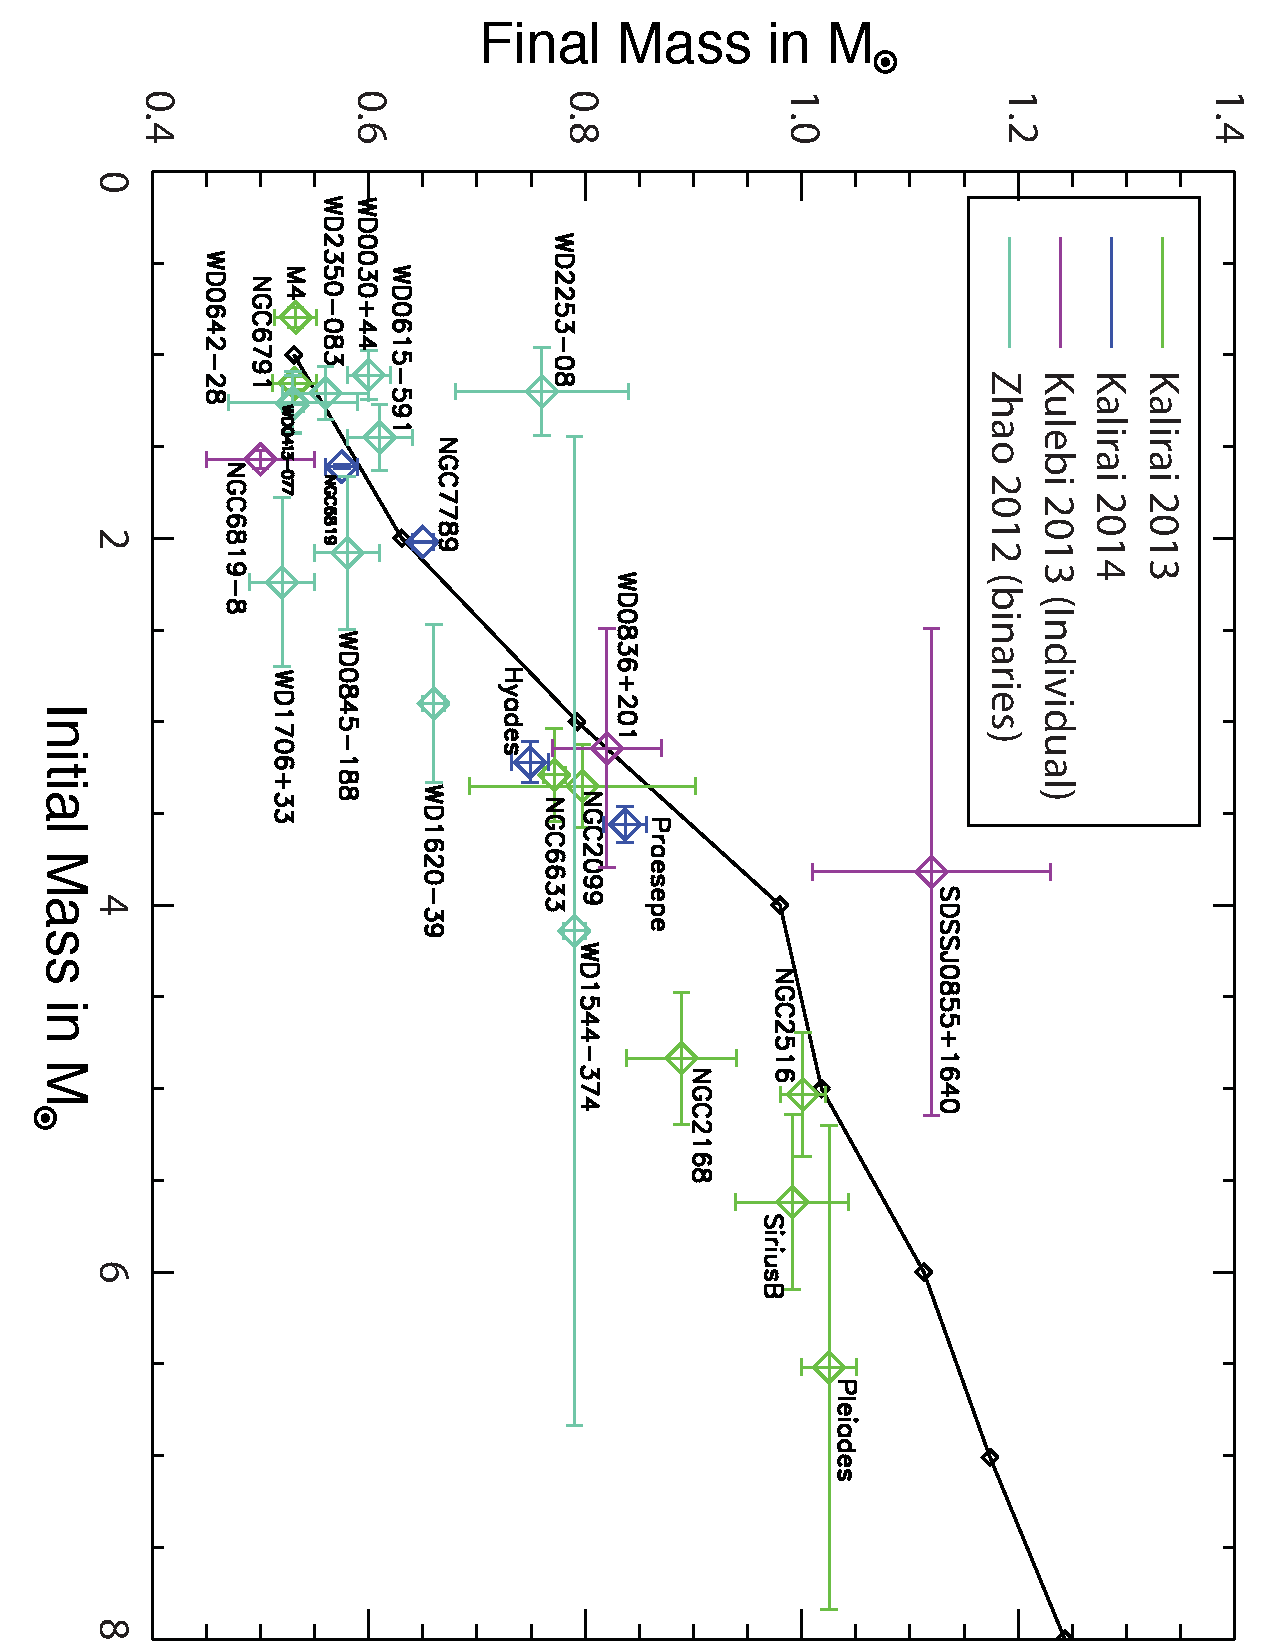
\includegraphics[width=0.35\textwidth, angle=90]{if_mod2.pdf}
\caption{ Initial final mass relation from observations and MESA calculations. The \citealt{kalirai2013a} and \citealt{kalirai2013b} points are averaged over the total observed white dwarfs in each respective cluster, while the \citealt{kulebi2013} and \citealt{zhao2012} points are taken from individual observations.}
\label{fig:ifrelation}
\end{figure} 

\begin{figure}
\centering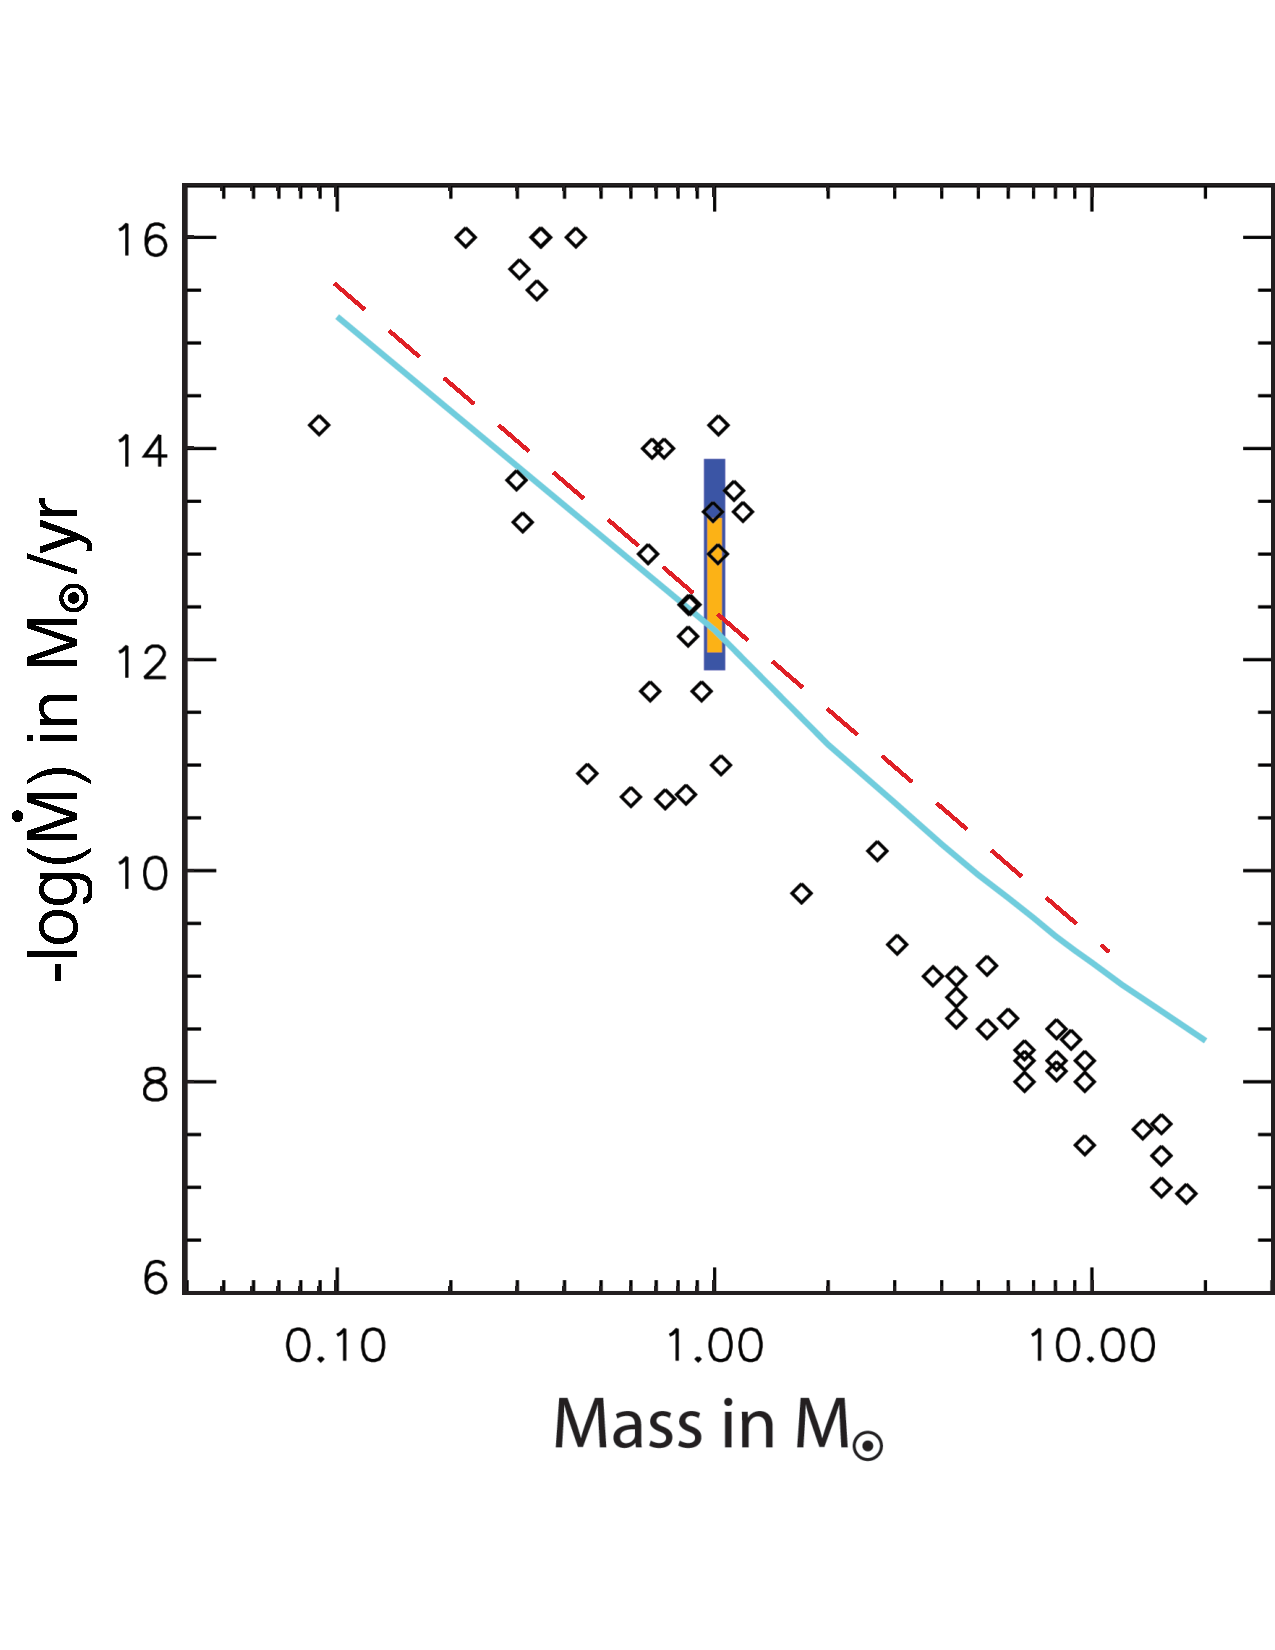
\includegraphics[width=0.46\textwidth]{mdotms_withAnalytic_mod3.pdf}
\caption{Mass loss rate estimates along the main sequence as a function of initial stellar mass.  Observational estimates are plotted as black diamonds \citep{cranmer2011,dejager1988,searle2008,waters1987,debes2006,badalyan1992,morin2008}.  The blue rectangle denotes the estimated variations in the solar mass loss rate \citep{wood2005}, and the yellow rectangle shows the observed variations in the mass loss rate of the Sun as a function of its X-ray activity \citep{cohen2011}.  The blue line shows the main sequence mass loss rate prescription used by MESA and the often derived analytical prescription is shown with the dashed red line. }
\label{fig:msmassloss}
\end{figure} 


\subsubsection{Wind Velocities}


\tikzmark{mainBodyStart2926}Shortening\tikzmark{mainBodyEnd2926} \tikzmark{mainBodyStart2927}here\tikzmark{mainBodyEnd2927} \tikzmark{mainBodyStart2928}as\tikzmark{mainBodyEnd2928} \tikzmark{mainBodyStart2929}well.\tikzmark{mainBodyEnd2929}

\subsection{Average Mass Loss and Wind Velocities as Model Inputs} \label{section:averages}

\tikzmark{mainBodyStart2930}To\tikzmark{mainBodyEnd2930} \tikzmark{mainBodyStart2931}finalize\tikzmark{mainBodyEnd2931} \tikzmark{mainBodyStart2932}our\tikzmark{mainBodyEnd2932} \tikzmark{mainBodyStart2933}mass\tikzmark{mainBodyEnd2933} \tikzmark{mainBodyStart2934}and\tikzmark{mainBodyEnd2934} \tikzmark{mainBodyStart2935}energy\tikzmark{mainBodyEnd2935} \tikzmark{mainBodyStart2936}injection\tikzmark{mainBodyEnd2936} \tikzmark{mainBodyStart2937}prescriptions\tikzmark{mainBodyEnd2937} \tikzmark{mainBodyStart2938}it\tikzmark{mainBodyEnd2938} \tikzmark{mainBodyStart2939}is\tikzmark{mainBodyEnd2939} \tikzmark{mainBodyStart2940}necessary\tikzmark{mainBodyEnd2940} \tikzmark{mainBodyStart2941}to\tikzmark{mainBodyEnd2941} \tikzmark{mainBodyStart2942}derive\tikzmark{mainBodyEnd2942} \tikzmark{mainBodyStart2943}an\tikzmark{mainBodyEnd2943} \tikzmark{mainBodyStart2944}averaged\tikzmark{mainBodyEnd2944} \tikzmark{mainBodyStart2945}mass\tikzmark{mainBodyEnd2945} \tikzmark{mainBodyStart2946}loss\tikzmark{mainBodyEnd2946} \tikzmark{mainBodyStart2947}rate\tikzmark{mainBodyEnd2947} \tikzmark{mainBodyStart2948}and\tikzmark{mainBodyEnd2948} \tikzmark{mainBodyStart2949}wind\tikzmark{mainBodyEnd2949} \tikzmark{mainBodyStart2950}velocity\tikzmark{mainBodyEnd2950} \tikzmark{mainBodyStart2951}during\tikzmark{mainBodyEnd2951} \tikzmark{mainBodyStart2952}each\tikzmark{mainBodyEnd2952} \tikzmark{mainBodyStart2953}phase\tikzmark{mainBodyEnd2953} \tikzmark{mainBodyStart2954}of\tikzmark{mainBodyEnd2954} \tikzmark{mainBodyStart2955}cluster\tikzmark{mainBodyEnd2955} \tikzmark{mainBodyStart2956}evolution\tikzmark{mainBodyEnd2956} \tikzmark{mainBodyStart2957}which\tikzmark{mainBodyEnd2957} \tikzmark{mainBodyStart2958}includes\tikzmark{mainBodyEnd2958} \tikzmark{mainBodyStart2959}contributions\tikzmark{mainBodyEnd2959} \tikzmark{mainBodyStart2960}from\tikzmark{mainBodyEnd2960} \tikzmark{mainBodyStart2961}the\tikzmark{mainBodyEnd2961} \tikzmark{mainBodyStart2962}stars\tikzmark{mainBodyEnd2962} \tikzmark{mainBodyStart2963}that\tikzmark{mainBodyEnd2963} \tikzmark{mainBodyStart2964}significantly\tikzmark{mainBodyEnd2964} \tikzmark{mainBodyStart2965}contribute\tikzmark{mainBodyEnd2965} \tikzmark{mainBodyStart2966}to\tikzmark{mainBodyEnd2966} \tikzmark{mainBodyStart2967}the\tikzmark{mainBodyEnd2967} \tikzmark{mainBodyStart2968}mass\tikzmark{mainBodyEnd2968} \tikzmark{mainBodyStart2969}and\tikzmark{mainBodyEnd2969} \tikzmark{mainBodyStart2970}kinetic\tikzmark{mainBodyEnd2970} \tikzmark{mainBodyStart2971}energy\tikzmark{mainBodyEnd2971} \tikzmark{mainBodyStart2972}injection\tikzmark{mainBodyEnd2972} \tikzmark{mainBodyStart2973}into\tikzmark{mainBodyEnd2973} \tikzmark{mainBodyStart2974}the\tikzmark{mainBodyEnd2974} \tikzmark{mainBodyStart2975}cluster.\tikzmark{mainBodyEnd2975}
\tikzmark{mainBodyStart2976}The\tikzmark{mainBodyEnd2976} \tikzmark{mainBodyStart2977}averaged\tikzmark{mainBodyEnd2977} \tikzmark{mainBodyStart2978}prescription\tikzmark{mainBodyEnd2978} \tikzmark{mainBodyStart2979}we\tikzmark{mainBodyEnd2979} \tikzmark{mainBodyStart2980}present\tikzmark{mainBodyEnd2980} \tikzmark{mainBodyStart2981}here\tikzmark{mainBodyEnd2981} \tikzmark{mainBodyStart2982}has\tikzmark{mainBodyEnd2982} \tikzmark{mainBodyStart2983}the\tikzmark{mainBodyEnd2983} \tikzmark{mainBodyStart2984}added\tikzmark{mainBodyEnd2984} \tikzmark{mainBodyStart2985}benefit\tikzmark{mainBodyEnd2985} \tikzmark{mainBodyStart2986}of\tikzmark{mainBodyEnd2986} \tikzmark{mainBodyStart2987}minimizing\tikzmark{mainBodyEnd2987} \tikzmark{mainBodyStart2988}the\tikzmark{mainBodyEnd2988} \tikzmark{mainBodyStart2989}effects\tikzmark{mainBodyEnd2989} \tikzmark{mainBodyStart2990}of\tikzmark{mainBodyEnd2990} \tikzmark{mainBodyStart2991}the\tikzmark{mainBodyEnd2991} \tikzmark{mainBodyStart2992}poorly\tikzmark{mainBodyEnd2992} \tikzmark{mainBodyStart2993}constrained,\tikzmark{mainBodyEnd2993} \tikzmark{mainBodyStart2994}rapidly\tikzmark{mainBodyEnd2994} \tikzmark{mainBodyStart2995}varying,\tikzmark{mainBodyEnd2995} \tikzmark{mainBodyStart2996}final\tikzmark{mainBodyEnd2996} \tikzmark{mainBodyStart2997}stages\tikzmark{mainBodyEnd2997} \tikzmark{mainBodyStart2998}of\tikzmark{mainBodyEnd2998} \tikzmark{mainBodyStart2999}a\tikzmark{mainBodyEnd2999} \tikzmark{mainBodyStart3000}star's\tikzmark{mainBodyEnd3000} \tikzmark{mainBodyStart3001}life\tikzmark{mainBodyEnd3001} \tikzmark{mainBodyCitationStart3002}\citep{pooley2006}\tikzmark{mainBodyCitationEnd3002}\tikzmark{mainBodyStart3003}.\tikzmark{mainBodyEnd3003}


\tikzmark{mainBodyStart3004}Note:\tikzmark{mainBodyEnd3004} \tikzmark{mainBodyStart3005}more\tikzmark{mainBodyEnd3005} \tikzmark{mainBodyStart3006}shortening\tikzmark{mainBodyEnd3006} \tikzmark{mainBodyStart3007}is\tikzmark{mainBodyEnd3007} \tikzmark{mainBodyStart3008}happening\tikzmark{mainBodyEnd3008} \tikzmark{mainBodyStart3009}here\tikzmark{mainBodyEnd3009} \tikzmark{mainBodyStart3010}too.\tikzmark{mainBodyEnd3010}

\section{Applications to Various Star Clusters} \label{section:applications}

\tikzmark{mainBodyStart3011}We\tikzmark{mainBodyEnd3011} \tikzmark{mainBodyStart3012}have\tikzmark{mainBodyEnd3012} \tikzmark{mainBodyStart3013}thus\tikzmark{mainBodyEnd3013} \tikzmark{mainBodyStart3014}far\tikzmark{mainBodyEnd3014} \tikzmark{mainBodyStart3015}kept\tikzmark{mainBodyEnd3015} \tikzmark{mainBodyStart3016}our\tikzmark{mainBodyEnd3016} \tikzmark{mainBodyStart3017}discussion\tikzmark{mainBodyEnd3017} \tikzmark{mainBodyStart3018}of\tikzmark{mainBodyEnd3018} \tikzmark{mainBodyStart3019}stellar\tikzmark{mainBodyEnd3019} \tikzmark{mainBodyStart3020}wind\tikzmark{mainBodyEnd3020} \tikzmark{mainBodyStart3021}retention\tikzmark{mainBodyEnd3021} \tikzmark{mainBodyStart3022}in\tikzmark{mainBodyEnd3022} \tikzmark{mainBodyStart3023}star\tikzmark{mainBodyEnd3023} \tikzmark{mainBodyStart3024}clusters\tikzmark{mainBodyEnd3024} \tikzmark{mainBodyStart3025}generalized\tikzmark{mainBodyEnd3025} \tikzmark{mainBodyStart3026}to\tikzmark{mainBodyEnd3026} \tikzmark{mainBodyStart3027}star\tikzmark{mainBodyEnd3027} \tikzmark{mainBodyStart3028}clusters\tikzmark{mainBodyEnd3028} \tikzmark{mainBodyStart3029}with\tikzmark{mainBodyEnd3029} \tikzmark{mainBodyStart3030}different\tikzmark{mainBodyEnd3030} \tikzmark{mainBodyStart3031}combinations\tikzmark{mainBodyEnd3031} \tikzmark{mainBodyStart3032}of\tikzmark{mainBodyEnd3032} \tikzmark{mainBodyStart3033}ages,\tikzmark{mainBodyEnd3033} \tikzmark{mainBodyStart3034}masses\tikzmark{mainBodyEnd3034} \tikzmark{mainBodyStart3035}and\tikzmark{mainBodyEnd3035} \tikzmark{mainBodyStart3036}velocity\tikzmark{mainBodyEnd3036} \tikzmark{mainBodyStart3037}dispersions.\tikzmark{mainBodyEnd3037}  \tikzmark{mainBodyStart3038}In\tikzmark{mainBodyEnd3038} \tikzmark{mainBodyStart3039}what\tikzmark{mainBodyEnd3039} \tikzmark{mainBodyStart3040}follows\tikzmark{mainBodyEnd3040} \tikzmark{mainBodyStart3041}we\tikzmark{mainBodyEnd3041} \tikzmark{mainBodyStart3042}discuss\tikzmark{mainBodyEnd3042} \tikzmark{mainBodyStart3043}the\tikzmark{mainBodyEnd3043} \tikzmark{mainBodyStart3044}implications\tikzmark{mainBodyEnd3044} \tikzmark{mainBodyStart3045}of\tikzmark{mainBodyEnd3045} \tikzmark{mainBodyStart3046}gas\tikzmark{mainBodyEnd3046} \tikzmark{mainBodyStart3047}retention\tikzmark{mainBodyEnd3047} \tikzmark{mainBodyStart3048}on\tikzmark{mainBodyEnd3048} \tikzmark{mainBodyStart3049}three\tikzmark{mainBodyEnd3049} \tikzmark{mainBodyStart3050}specific\tikzmark{mainBodyEnd3050} \tikzmark{mainBodyStart3051}groups\tikzmark{mainBodyEnd3051} \tikzmark{mainBodyStart3052}of\tikzmark{mainBodyEnd3052} \tikzmark{mainBodyStart3053}star\tikzmark{mainBodyEnd3053} \tikzmark{mainBodyStart3054}clusters\tikzmark{mainBodyEnd3054} \tikzmark{mainBodyStart3055}-\tikzmark{mainBodyEnd3055} \tikzmark{mainBodyStart3056}Young\tikzmark{mainBodyEnd3056} \tikzmark{mainBodyStart3057}Massive\tikzmark{mainBodyEnd3057} \tikzmark{mainBodyStart3058}Clusters,\tikzmark{mainBodyEnd3058} \tikzmark{mainBodyStart3059}Intermediate\tikzmark{mainBodyEnd3059} \tikzmark{mainBodyStart3060}Age\tikzmark{mainBodyEnd3060} \tikzmark{mainBodyStart3061}Clusters,\tikzmark{mainBodyEnd3061} \tikzmark{mainBodyStart3062}and\tikzmark{mainBodyEnd3062} \tikzmark{mainBodyStart3063}Globular\tikzmark{mainBodyEnd3063} \tikzmark{mainBodyStart3064}Clusters\tikzmark{mainBodyEnd3064} \tikzmark{mainBodyStart3065}-\tikzmark{mainBodyEnd3065} \tikzmark{mainBodyStart3066}and\tikzmark{mainBodyEnd3066} \tikzmark{mainBodyStart3067}provide\tikzmark{mainBodyEnd3067} \tikzmark{mainBodyStart3068}limits\tikzmark{mainBodyEnd3068} \tikzmark{mainBodyStart3069}on\tikzmark{mainBodyEnd3069} \tikzmark{mainBodyStart3070}how\tikzmark{mainBodyEnd3070} \tikzmark{mainBodyStart3071}stellar\tikzmark{mainBodyEnd3071} \tikzmark{mainBodyStart3072}wind\tikzmark{mainBodyEnd3072} \tikzmark{mainBodyStart3073}retention\tikzmark{mainBodyEnd3073} \tikzmark{mainBodyStart3074}can\tikzmark{mainBodyEnd3074} \tikzmark{mainBodyStart3075}effect\tikzmark{mainBodyEnd3075} \tikzmark{mainBodyStart3076}their\tikzmark{mainBodyEnd3076} \tikzmark{mainBodyStart3077}star\tikzmark{mainBodyEnd3077} \tikzmark{mainBodyStart3078}formation\tikzmark{mainBodyEnd3078} \tikzmark{mainBodyStart3079}histories.\tikzmark{mainBodyEnd3079}


\subsection{Young Massive Clusters: Age $\lesssim$1~Gyr}

\tikzmark{mainBodyStart3080}Young,\tikzmark{mainBodyEnd3080} \tikzmark{mainBodyStart3081}massive\tikzmark{mainBodyEnd3081} \tikzmark{mainBodyStart3082}star\tikzmark{mainBodyEnd3082} \tikzmark{mainBodyStart3083}clusters\tikzmark{mainBodyEnd3083} \tikzmark{mainBodyStart3084}(YMCs)\tikzmark{mainBodyEnd3084} \tikzmark{mainBodyStart3085}are\tikzmark{mainBodyEnd3085} \tikzmark{mainBodyStart3086}ubiquitous\tikzmark{mainBodyEnd3086} \tikzmark{mainBodyStart3087}in\tikzmark{mainBodyEnd3087} \tikzmark{mainBodyStart3088}the\tikzmark{mainBodyEnd3088} \tikzmark{mainBodyStart3089}nearby\tikzmark{mainBodyEnd3089} \tikzmark{mainBodyStart3090}Small\tikzmark{mainBodyEnd3090} \tikzmark{mainBodyStart3091}and\tikzmark{mainBodyEnd3091} \tikzmark{mainBodyStart3092}Large\tikzmark{mainBodyEnd3092} \tikzmark{mainBodyStart3093}Magellanic\tikzmark{mainBodyEnd3093} \tikzmark{mainBodyStart3094}Clouds\tikzmark{mainBodyEnd3094} \tikzmark{mainBodyCitationStart3095}\citep{goud2014}\tikzmark{mainBodyCitationEnd3095} \tikzmark{mainBodyStart3096}and\tikzmark{mainBodyEnd3096} \tikzmark{mainBodyStart3097}are\tikzmark{mainBodyEnd3097} \tikzmark{mainBodyStart3098}also\tikzmark{mainBodyEnd3098} \tikzmark{mainBodyStart3099}found\tikzmark{mainBodyEnd3099} \tikzmark{mainBodyStart3100}in\tikzmark{mainBodyEnd3100} \tikzmark{mainBodyStart3101}recent\tikzmark{mainBodyEnd3101} \tikzmark{mainBodyStart3102}(\tikzmark{mainBodyEnd3102}\tikzmark{mainBodyInlineStart3103}$\lesssim$\tikzmark{mainBodyInlineEnd3103}\tikzmark{mainBodyStart3104}1~Gyr)\tikzmark{mainBodyEnd3104} \tikzmark{mainBodyStart3105}mergers\tikzmark{mainBodyEnd3105} \tikzmark{mainBodyStart3106}like\tikzmark{mainBodyEnd3106} \tikzmark{mainBodyStart3107}the\tikzmark{mainBodyEnd3107} \tikzmark{mainBodyStart3108}Antennae\tikzmark{mainBodyEnd3108} \tikzmark{mainBodyStart3109}galaxies\tikzmark{mainBodyEnd3109} \tikzmark{mainBodyCitationStart3110}\citep{whitmore2007}\tikzmark{mainBodyCitationEnd3110}\tikzmark{mainBodyStart3111}.\tikzmark{mainBodyEnd3111}  \tikzmark{mainBodyStart3112}As\tikzmark{mainBodyEnd3112} \tikzmark{mainBodyStart3113}one\tikzmark{mainBodyEnd3113} \tikzmark{mainBodyStart3114}of\tikzmark{mainBodyEnd3114} \tikzmark{mainBodyStart3115}the\tikzmark{mainBodyEnd3115} \tikzmark{mainBodyStart3116}canditates\tikzmark{mainBodyEnd3116} \tikzmark{mainBodyStart3117}for\tikzmark{mainBodyEnd3117} \tikzmark{mainBodyStart3118}proto-Globular\tikzmark{mainBodyEnd3118} \tikzmark{mainBodyStart3119}Clusters,\tikzmark{mainBodyEnd3119} \tikzmark{mainBodyStart3120}the\tikzmark{mainBodyEnd3120} \tikzmark{mainBodyStart3121}gas\tikzmark{mainBodyEnd3121} \tikzmark{mainBodyStart3122}content\tikzmark{mainBodyEnd3122} \tikzmark{mainBodyStart3123}and\tikzmark{mainBodyEnd3123} \tikzmark{mainBodyStart3124}star\tikzmark{mainBodyEnd3124} \tikzmark{mainBodyStart3125}formation\tikzmark{mainBodyEnd3125} \tikzmark{mainBodyStart3126}histories\tikzmark{mainBodyEnd3126} \tikzmark{mainBodyStart3127}of\tikzmark{mainBodyEnd3127} \tikzmark{mainBodyStart3128}these\tikzmark{mainBodyEnd3128} \tikzmark{mainBodyStart3129}objects\tikzmark{mainBodyEnd3129} \tikzmark{mainBodyStart3130}are\tikzmark{mainBodyEnd3130} \tikzmark{mainBodyStart3131}a\tikzmark{mainBodyEnd3131} \tikzmark{mainBodyStart3132}subject\tikzmark{mainBodyEnd3132} \tikzmark{mainBodyStart3133}of\tikzmark{mainBodyEnd3133} \tikzmark{mainBodyStart3134}much\tikzmark{mainBodyEnd3134} \tikzmark{mainBodyStart3135}interest\tikzmark{mainBodyEnd3135} \tikzmark{mainBodyCitationStart3136}\citep[e.g.][]{zwart2010}\tikzmark{mainBodyCitationEnd3136}\tikzmark{mainBodyStart3137}.\tikzmark{mainBodyEnd3137}

\subsubsection{Current Gas Content} \label{section:YMCcurrent}

 \tikzmark{mainBodyStart3138}During\tikzmark{mainBodyEnd3138} \tikzmark{mainBodyStart3139}the\tikzmark{mainBodyEnd3139} \tikzmark{mainBodyStart3140}time\tikzmark{mainBodyEnd3140} \tikzmark{mainBodyStart3141}span\tikzmark{mainBodyEnd3141} \tikzmark{mainBodyStart3142}of\tikzmark{mainBodyEnd3142} \tikzmark{mainBodyStart3143}the\tikzmark{mainBodyEnd3143} \tikzmark{mainBodyStart3144}typical\tikzmark{mainBodyEnd3144} \tikzmark{mainBodyStart3145}ages\tikzmark{mainBodyEnd3145} \tikzmark{mainBodyStart3146}of\tikzmark{mainBodyEnd3146} \tikzmark{mainBodyStart3147}YMCs\tikzmark{mainBodyEnd3147} \tikzmark{mainBodyStart3148}(10s-100s~Myrs)\tikzmark{mainBodyEnd3148} \tikzmark{mainBodyStart3149}Figures\tikzmark{mainBodyEnd3149} \tikzmark{mainBodyrefStart3150}\ref{fig:fig4}\tikzmark{mainBodyrefEnd3150} \tikzmark{mainBodyStart3151}-\tikzmark{mainBodyEnd3151} \tikzmark{mainBodyrefStart3152}\ref{fig:memcontour}\tikzmark{mainBodyrefEnd3152} \tikzmark{mainBodyStart3153}show\tikzmark{mainBodyEnd3153} \tikzmark{mainBodyStart3154}little\tikzmark{mainBodyEnd3154} \tikzmark{mainBodyStart3155}mass\tikzmark{mainBodyEnd3155} \tikzmark{mainBodyStart3156}retention\tikzmark{mainBodyEnd3156} \tikzmark{mainBodyStart3157}and\tikzmark{mainBodyEnd3157} \tikzmark{mainBodyStart3158}star\tikzmark{mainBodyEnd3158} \tikzmark{mainBodyStart3159}formation\tikzmark{mainBodyEnd3159} \tikzmark{mainBodyStart3160}in\tikzmark{mainBodyEnd3160} \tikzmark{mainBodyStart3161}all\tikzmark{mainBodyEnd3161} \tikzmark{mainBodyStart3162}but\tikzmark{mainBodyEnd3162} \tikzmark{mainBodyStart3163}the\tikzmark{mainBodyEnd3163} \tikzmark{mainBodyStart3164}most\tikzmark{mainBodyEnd3164} \tikzmark{mainBodyStart3165}compact\tikzmark{mainBodyEnd3165} \tikzmark{mainBodyStart3166}stellar\tikzmark{mainBodyEnd3166} \tikzmark{mainBodyStart3167}clusters.\tikzmark{mainBodyEnd3167}
 \tikzmark{mainBodyStart3168}This\tikzmark{mainBodyEnd3168} \tikzmark{mainBodyStart3169}results\tikzmark{mainBodyEnd3169} \tikzmark{mainBodyStart3170}from\tikzmark{mainBodyEnd3170} \tikzmark{mainBodyStart3171}the\tikzmark{mainBodyEnd3171} \tikzmark{mainBodyStart3172}fast\tikzmark{mainBodyEnd3172} \tikzmark{mainBodyStart3173}winds\tikzmark{mainBodyEnd3173} \tikzmark{mainBodyStart3174}from\tikzmark{mainBodyEnd3174} \tikzmark{mainBodyStart3175}main\tikzmark{mainBodyEnd3175} \tikzmark{mainBodyStart3176}sequence\tikzmark{mainBodyEnd3176} \tikzmark{mainBodyStart3177}O\tikzmark{mainBodyEnd3177} \tikzmark{mainBodyStart3178}and\tikzmark{mainBodyEnd3178} \tikzmark{mainBodyStart3179}B\tikzmark{mainBodyEnd3179} \tikzmark{mainBodyStart3180}stars\tikzmark{mainBodyEnd3180} \tikzmark{mainBodyStart3181}as\tikzmark{mainBodyEnd3181} \tikzmark{mainBodyStart3182}shown\tikzmark{mainBodyEnd3182} \tikzmark{mainBodyStart3183}in\tikzmark{mainBodyEnd3183} \tikzmark{mainBodyStart3184}Figure\tikzmark{mainBodyEnd3184} \tikzmark{mainBodyrefStart3185}\ref{fig:fig1}\tikzmark{mainBodyrefEnd3185} \tikzmark{mainBodyStart3186}for\tikzmark{mainBodyEnd3186} \tikzmark{mainBodyStart3187}ages\tikzmark{mainBodyEnd3187} \tikzmark{mainBodyInlineStart3188}$\lesssim 20$\tikzmark{mainBodyInlineEnd3188}\tikzmark{mainBodyStart3189}~Myrs,\tikzmark{mainBodyEnd3189} \tikzmark{mainBodyStart3190}and\tikzmark{mainBodyEnd3190} \tikzmark{mainBodyStart3191}the\tikzmark{mainBodyEnd3191} \tikzmark{mainBodyStart3192}lack\tikzmark{mainBodyEnd3192} \tikzmark{mainBodyStart3193}of\tikzmark{mainBodyEnd3193} \tikzmark{mainBodyStart3194}sufficient\tikzmark{mainBodyEnd3194} \tikzmark{mainBodyStart3195}gas\tikzmark{mainBodyEnd3195} \tikzmark{mainBodyStart3196}accumulation\tikzmark{mainBodyEnd3196} \tikzmark{mainBodyStart3197}time\tikzmark{mainBodyEnd3197} \tikzmark{mainBodyStart3198}to\tikzmark{mainBodyEnd3198} \tikzmark{mainBodyStart3199}initiate\tikzmark{mainBodyEnd3199} \tikzmark{mainBodyStart3200}runaway\tikzmark{mainBodyEnd3200} \tikzmark{mainBodyStart3201}cooling\tikzmark{mainBodyEnd3201} \tikzmark{mainBodyStart3202}and\tikzmark{mainBodyEnd3202} \tikzmark{mainBodyStart3203}collapse\tikzmark{mainBodyEnd3203} \tikzmark{mainBodyStart3204}for\tikzmark{mainBodyEnd3204} \tikzmark{mainBodyStart3205}clusters\tikzmark{mainBodyEnd3205} \tikzmark{mainBodyStart3206}with\tikzmark{mainBodyEnd3206} \tikzmark{mainBodyInlineStart3207}$20 \lesssim{\rm age/Myrs} \lesssim 500$\tikzmark{mainBodyInlineEnd3207}\tikzmark{mainBodyStart3208}.\tikzmark{mainBodyEnd3208}
 \tikzmark{mainBodyStart3209}For\tikzmark{mainBodyEnd3209} \tikzmark{mainBodyStart3210}clusters\tikzmark{mainBodyEnd3210} \tikzmark{mainBodyStart3211}with\tikzmark{mainBodyEnd3211} \tikzmark{mainBodyStart3212}large\tikzmark{mainBodyEnd3212} \tikzmark{mainBodyStart3213}velocity\tikzmark{mainBodyEnd3213} \tikzmark{mainBodyStart3214}dispersions,\tikzmark{mainBodyEnd3214} \tikzmark{mainBodyInlineStart3215}$\sigma_v \gtrsim 35 \, {\rm km s^{-1}}$\tikzmark{mainBodyInlineEnd3215}\tikzmark{mainBodyStart3216},\tikzmark{mainBodyEnd3216} \tikzmark{mainBodyStart3217}while\tikzmark{mainBodyEnd3217} \tikzmark{mainBodyStart3218}some\tikzmark{mainBodyEnd3218} \tikzmark{mainBodyStart3219}gas\tikzmark{mainBodyEnd3219} \tikzmark{mainBodyStart3220}mass\tikzmark{mainBodyEnd3220} \tikzmark{mainBodyStart3221}is\tikzmark{mainBodyEnd3221} \tikzmark{mainBodyStart3222}retained\tikzmark{mainBodyEnd3222} \tikzmark{mainBodyStart3223}and\tikzmark{mainBodyEnd3223} \tikzmark{mainBodyStart3224}star\tikzmark{mainBodyEnd3224} \tikzmark{mainBodyStart3225}formation\tikzmark{mainBodyEnd3225} \tikzmark{mainBodyStart3226}is\tikzmark{mainBodyEnd3226} \tikzmark{mainBodyStart3227}triggered,\tikzmark{mainBodyEnd3227} \tikzmark{mainBodyStart3228}less\tikzmark{mainBodyEnd3228} \tikzmark{mainBodyStart3229}than\tikzmark{mainBodyEnd3229} \tikzmark{mainBodyInlineStart3230}$\approx 2$\tikzmark{mainBodyInlineEnd3230}\tikzmark{mainBodyStart3231}\%\tikzmark{mainBodyEnd3231} \tikzmark{mainBodyStart3232}of\tikzmark{mainBodyEnd3232} \tikzmark{mainBodyStart3233}the\tikzmark{mainBodyEnd3233} \tikzmark{mainBodyStart3234}original\tikzmark{mainBodyEnd3234} \tikzmark{mainBodyStart3235}cluster's\tikzmark{mainBodyEnd3235} \tikzmark{mainBodyStart3236}mass\tikzmark{mainBodyEnd3236} \tikzmark{mainBodyStart3237}is\tikzmark{mainBodyEnd3237} \tikzmark{mainBodyStart3238}available\tikzmark{mainBodyEnd3238} \tikzmark{mainBodyStart3239}for\tikzmark{mainBodyEnd3239} \tikzmark{mainBodyStart3240}star\tikzmark{mainBodyEnd3240} \tikzmark{mainBodyStart3241}formation.\tikzmark{mainBodyEnd3241}

 \tikzmark{mainBodyStart3242}In\tikzmark{mainBodyEnd3242} \tikzmark{mainBodyStart3243}such\tikzmark{mainBodyEnd3243} \tikzmark{mainBodyStart3244}clusters\tikzmark{mainBodyEnd3244} \tikzmark{mainBodyStart3245}we\tikzmark{mainBodyEnd3245} \tikzmark{mainBodyStart3246}expect\tikzmark{mainBodyEnd3246} \tikzmark{mainBodyStart3247}several\tikzmark{mainBodyEnd3247} \tikzmark{mainBodyStart3248}additional\tikzmark{mainBodyEnd3248} \tikzmark{mainBodyStart3249}mechanisms\tikzmark{mainBodyEnd3249} \tikzmark{mainBodyStart3250}to\tikzmark{mainBodyEnd3250} \tikzmark{mainBodyStart3251}add\tikzmark{mainBodyEnd3251} \tikzmark{mainBodyStart3252}significantly\tikzmark{mainBodyEnd3252} \tikzmark{mainBodyStart3253}to\tikzmark{mainBodyEnd3253} \tikzmark{mainBodyStart3254}the\tikzmark{mainBodyEnd3254} \tikzmark{mainBodyStart3255}energy\tikzmark{mainBodyEnd3255} \tikzmark{mainBodyStart3256}injection\tikzmark{mainBodyEnd3256} \tikzmark{mainBodyStart3257}rate\tikzmark{mainBodyEnd3257} \tikzmark{mainBodyStart3258}in\tikzmark{mainBodyEnd3258} \tikzmark{mainBodyStart3259}the\tikzmark{mainBodyEnd3259} \tikzmark{mainBodyStart3260}intercluster\tikzmark{mainBodyEnd3260} \tikzmark{mainBodyStart3261}gas.\tikzmark{mainBodyEnd3261}
 \tikzmark{mainBodyStart3262}As\tikzmark{mainBodyEnd3262} \tikzmark{mainBodyStart3263}shown\tikzmark{mainBodyEnd3263} \tikzmark{mainBodyStart3264}in\tikzmark{mainBodyEnd3264} \tikzmark{mainBodyCitationStart3265}\cite{calura2015}\tikzmark{mainBodyCitationEnd3265} \tikzmark{mainBodyStart3266}SNe\tikzmark{mainBodyEnd3266} \tikzmark{mainBodyStart3267}can\tikzmark{mainBodyEnd3267} \tikzmark{mainBodyStart3268}be\tikzmark{mainBodyEnd3268} \tikzmark{mainBodyStart3269}an\tikzmark{mainBodyEnd3269} \tikzmark{mainBodyStart3270}effective\tikzmark{mainBodyEnd3270} \tikzmark{mainBodyStart3271}avenue\tikzmark{mainBodyEnd3271} \tikzmark{mainBodyStart3272}to\tikzmark{mainBodyEnd3272} \tikzmark{mainBodyStart3273}assist\tikzmark{mainBodyEnd3273} \tikzmark{mainBodyStart3274}in\tikzmark{mainBodyEnd3274} \tikzmark{mainBodyStart3275}the\tikzmark{mainBodyEnd3275} \tikzmark{mainBodyStart3276}removal\tikzmark{mainBodyEnd3276} \tikzmark{mainBodyStart3277}of\tikzmark{mainBodyEnd3277} \tikzmark{mainBodyStart3278}gas\tikzmark{mainBodyEnd3278} \tikzmark{mainBodyStart3279}from\tikzmark{mainBodyEnd3279} \tikzmark{mainBodyStart3280}stellar\tikzmark{mainBodyEnd3280} \tikzmark{mainBodyStart3281}clusters,\tikzmark{mainBodyEnd3281} \tikzmark{mainBodyStart3282}though\tikzmark{mainBodyEnd3282} \tikzmark{mainBodyStart3283}in\tikzmark{mainBodyEnd3283} \tikzmark{mainBodyStart3284}some\tikzmark{mainBodyEnd3284} \tikzmark{mainBodyStart3285}systems\tikzmark{mainBodyEnd3285} \tikzmark{mainBodyStart3286}SNe\tikzmark{mainBodyEnd3286} \tikzmark{mainBodyStart3287}alone\tikzmark{mainBodyEnd3287} \tikzmark{mainBodyStart3288}may\tikzmark{mainBodyEnd3288} \tikzmark{mainBodyStart3289}not\tikzmark{mainBodyEnd3289} \tikzmark{mainBodyStart3290}be\tikzmark{mainBodyEnd3290} \tikzmark{mainBodyStart3291}able\tikzmark{mainBodyEnd3291} \tikzmark{mainBodyStart3292}to\tikzmark{mainBodyEnd3292} \tikzmark{mainBodyStart3293}fully\tikzmark{mainBodyEnd3293} \tikzmark{mainBodyStart3294}remove\tikzmark{mainBodyEnd3294} \tikzmark{mainBodyStart3295}gas\tikzmark{mainBodyEnd3295} \tikzmark{mainBodyStart3296}from\tikzmark{mainBodyEnd3296} \tikzmark{mainBodyStart3297}young\tikzmark{mainBodyEnd3297} \tikzmark{mainBodyStart3298}clusters\tikzmark{mainBodyEnd3298} \tikzmark{mainBodyCitationStart3299}\citep{krause2013}\tikzmark{mainBodyCitationEnd3299}\tikzmark{mainBodyStart3300}.\tikzmark{mainBodyEnd3300}
 \tikzmark{mainBodyStart3301}In\tikzmark{mainBodyEnd3301} \tikzmark{mainBodyStart3302}addition,\tikzmark{mainBodyEnd3302} \tikzmark{mainBodyStart3303}accretion\tikzmark{mainBodyEnd3303} \tikzmark{mainBodyStart3304}onto\tikzmark{mainBodyEnd3304} \tikzmark{mainBodyStart3305}compact\tikzmark{mainBodyEnd3305} \tikzmark{mainBodyStart3306}objects\tikzmark{mainBodyEnd3306} \tikzmark{mainBodyStart3307}may\tikzmark{mainBodyEnd3307} \tikzmark{mainBodyStart3308}be\tikzmark{mainBodyEnd3308} \tikzmark{mainBodyStart3309}able\tikzmark{mainBodyEnd3309} \tikzmark{mainBodyStart3310}to\tikzmark{mainBodyEnd3310} \tikzmark{mainBodyStart3311}clear\tikzmark{mainBodyEnd3311} \tikzmark{mainBodyStart3312}gas\tikzmark{mainBodyEnd3312} \tikzmark{mainBodyStart3313}within\tikzmark{mainBodyEnd3313} \tikzmark{mainBodyStart3314}YMCs\tikzmark{mainBodyEnd3314} \tikzmark{mainBodyStart3315}on\tikzmark{mainBodyEnd3315} \tikzmark{mainBodyStart3316}time\tikzmark{mainBodyEnd3316} \tikzmark{mainBodyStart3317}scales\tikzmark{mainBodyEnd3317} \tikzmark{mainBodyStart3318}as\tikzmark{mainBodyEnd3318} \tikzmark{mainBodyStart3319}small\tikzmark{mainBodyEnd3319} \tikzmark{mainBodyStart3320}as\tikzmark{mainBodyEnd3320} \tikzmark{mainBodyStart3321}10~Myrs\tikzmark{mainBodyEnd3321} \tikzmark{mainBodyCitationStart3322}\citep{leigh2013a}\tikzmark{mainBodyCitationEnd3322}\tikzmark{mainBodyStart3323}.\tikzmark{mainBodyEnd3323}
 \tikzmark{mainBodyStart3324}Finally,\tikzmark{mainBodyEnd3324} \tikzmark{mainBodyStart3325}Lyman-Werner\tikzmark{mainBodyEnd3325} \tikzmark{mainBodyStart3326}flux\tikzmark{mainBodyEnd3326} \tikzmark{mainBodyStart3327}from\tikzmark{mainBodyEnd3327} \tikzmark{mainBodyStart3328}massive\tikzmark{mainBodyEnd3328} \tikzmark{mainBodyStart3329}stars\tikzmark{mainBodyEnd3329} \tikzmark{mainBodyStart3330}further\tikzmark{mainBodyEnd3330} \tikzmark{mainBodyStart3331}inhibits\tikzmark{mainBodyEnd3331} \tikzmark{mainBodyStart3332}star\tikzmark{mainBodyEnd3332} \tikzmark{mainBodyStart3333}formation\tikzmark{mainBodyEnd3333} \tikzmark{mainBodyStart3334}by\tikzmark{mainBodyEnd3334} \tikzmark{mainBodyStart3335}dissassociating\tikzmark{mainBodyEnd3335} \tikzmark{mainBodyStart3336}molecular\tikzmark{mainBodyEnd3336} \tikzmark{mainBodyStart3337}hydrogen\tikzmark{mainBodyEnd3337} \tikzmark{mainBodyStart3338}in\tikzmark{mainBodyEnd3338} \tikzmark{mainBodyStart3339}these\tikzmark{mainBodyEnd3339} \tikzmark{mainBodyStart3340}young\tikzmark{mainBodyEnd3340} \tikzmark{mainBodyStart3341}systems\tikzmark{mainBodyEnd3341} \tikzmark{mainBodyCitationStart3342}\citep{ten1986,conroy2011b,krause2013}\tikzmark{mainBodyCitationEnd3342}\tikzmark{mainBodyStart3343}.\tikzmark{mainBodyEnd3343}
 \tikzmark{mainBodyStart3344}Therefore,\tikzmark{mainBodyEnd3344} \tikzmark{mainBodyStart3345}we\tikzmark{mainBodyEnd3345} \tikzmark{mainBodyStart3346}conclude\tikzmark{mainBodyEnd3346} \tikzmark{mainBodyStart3347}that\tikzmark{mainBodyEnd3347} \tikzmark{mainBodyStart3348}our\tikzmark{mainBodyEnd3348} \tikzmark{mainBodyStart3349}estimates\tikzmark{mainBodyEnd3349} \tikzmark{mainBodyStart3350}of\tikzmark{mainBodyEnd3350} \tikzmark{mainBodyStart3351}gas\tikzmark{mainBodyEnd3351} \tikzmark{mainBodyStart3352}retention\tikzmark{mainBodyEnd3352} \tikzmark{mainBodyStart3353}on\tikzmark{mainBodyEnd3353} \tikzmark{mainBodyStart3354}the\tikzmark{mainBodyEnd3354} \tikzmark{mainBodyStart3355}order\tikzmark{mainBodyEnd3355} \tikzmark{mainBodyStart3356}of\tikzmark{mainBodyEnd3356} \tikzmark{mainBodyStart3357}a\tikzmark{mainBodyEnd3357} \tikzmark{mainBodyStart3358}few\tikzmark{mainBodyEnd3358} \tikzmark{mainBodyStart3359}percent\tikzmark{mainBodyEnd3359} \tikzmark{mainBodyStart3360}are\tikzmark{mainBodyEnd3360} \tikzmark{mainBodyStart3361}upper\tikzmark{mainBodyEnd3361} \tikzmark{mainBodyStart3362}limits\tikzmark{mainBodyEnd3362} \tikzmark{mainBodyStart3363}for\tikzmark{mainBodyEnd3363} \tikzmark{mainBodyStart3364}the\tikzmark{mainBodyEnd3364} \tikzmark{mainBodyStart3365}total\tikzmark{mainBodyEnd3365} \tikzmark{mainBodyStart3366}mass\tikzmark{mainBodyEnd3366} \tikzmark{mainBodyStart3367}retained\tikzmark{mainBodyEnd3367} \tikzmark{mainBodyStart3368}from\tikzmark{mainBodyEnd3368} \tikzmark{mainBodyStart3369}stellar\tikzmark{mainBodyEnd3369} \tikzmark{mainBodyStart3370}wind\tikzmark{mainBodyEnd3370} \tikzmark{mainBodyStart3371}ejecta\tikzmark{mainBodyEnd3371} \tikzmark{mainBodyStart3372}within\tikzmark{mainBodyEnd3372} \tikzmark{mainBodyStart3373}YMCs.\tikzmark{mainBodyEnd3373}

 \tikzmark{mainBodyStart3374}Such\tikzmark{mainBodyEnd3374} \tikzmark{mainBodyStart3375}a\tikzmark{mainBodyEnd3375} \tikzmark{mainBodyStart3376}small\tikzmark{mainBodyEnd3376} \tikzmark{mainBodyStart3377}amount\tikzmark{mainBodyEnd3377} \tikzmark{mainBodyStart3378}of\tikzmark{mainBodyEnd3378} \tikzmark{mainBodyStart3379}gas\tikzmark{mainBodyEnd3379} \tikzmark{mainBodyStart3380}retention\tikzmark{mainBodyEnd3380} \tikzmark{mainBodyStart3381}is\tikzmark{mainBodyEnd3381} \tikzmark{mainBodyStart3382}broadly\tikzmark{mainBodyEnd3382} \tikzmark{mainBodyStart3383}consistent\tikzmark{mainBodyEnd3383} \tikzmark{mainBodyStart3384}with\tikzmark{mainBodyEnd3384} \tikzmark{mainBodyStart3385}both\tikzmark{mainBodyEnd3385} \tikzmark{mainBodyStart3386}observations\tikzmark{mainBodyEnd3386} \tikzmark{mainBodyStart3387}and\tikzmark{mainBodyEnd3387} \tikzmark{mainBodyStart3388}more\tikzmark{mainBodyEnd3388} \tikzmark{mainBodyStart3389}complex\tikzmark{mainBodyEnd3389} \tikzmark{mainBodyStart3390}simulations.\tikzmark{mainBodyEnd3390}
 \tikzmark{mainBodyStart3391}Recent\tikzmark{mainBodyEnd3391} \tikzmark{mainBodyStart3392}observations\tikzmark{mainBodyEnd3392} \tikzmark{mainBodyStart3393}which\tikzmark{mainBodyEnd3393} \tikzmark{mainBodyStart3394}show\tikzmark{mainBodyEnd3394} \tikzmark{mainBodyStart3395}little\tikzmark{mainBodyEnd3395} \tikzmark{mainBodyStart3396}gas\tikzmark{mainBodyEnd3396} \tikzmark{mainBodyStart3397}in\tikzmark{mainBodyEnd3397} \tikzmark{mainBodyStart3398}all\tikzmark{mainBodyEnd3398} \tikzmark{mainBodyStart3399}but\tikzmark{mainBodyEnd3399} \tikzmark{mainBodyStart3400}the\tikzmark{mainBodyEnd3400} \tikzmark{mainBodyStart3401}most\tikzmark{mainBodyEnd3401} \tikzmark{mainBodyStart3402}compact\tikzmark{mainBodyEnd3402} \tikzmark{mainBodyStart3403}clusters\tikzmark{mainBodyEnd3403} \tikzmark{mainBodyCitationStart3404}\citep{bastian2014a,cabrera2015,krui2015,longmore2015}\tikzmark{mainBodyCitationEnd3404}\tikzmark{mainBodyStart3405},\tikzmark{mainBodyEnd3405} \tikzmark{mainBodyStart3406}though\tikzmark{mainBodyEnd3406} \tikzmark{mainBodyStart3407}observations\tikzmark{mainBodyEnd3407} \tikzmark{mainBodyStart3408}at\tikzmark{mainBodyEnd3408} \tikzmark{mainBodyStart3409}high\tikzmark{mainBodyEnd3409} \tikzmark{mainBodyStart3410}redshift\tikzmark{mainBodyEnd3410} \tikzmark{mainBodyStart3411}are\tikzmark{mainBodyEnd3411} \tikzmark{mainBodyStart3412}challenging\tikzmark{mainBodyEnd3412} \tikzmark{mainBodyCitationStart3413}\citep{longmore2015}\tikzmark{mainBodyCitationEnd3413}\tikzmark{mainBodyStart3414}.\tikzmark{mainBodyEnd3414}
 \tikzmark{mainBodyStart3415}Our\tikzmark{mainBodyEnd3415} \tikzmark{mainBodyStart3416}results\tikzmark{mainBodyEnd3416} \tikzmark{mainBodyStart3417}are\tikzmark{mainBodyEnd3417} \tikzmark{mainBodyStart3418}also\tikzmark{mainBodyEnd3418} \tikzmark{mainBodyStart3419}consistent\tikzmark{mainBodyEnd3419} \tikzmark{mainBodyStart3420}with\tikzmark{mainBodyEnd3420} \tikzmark{mainBodyStart3421}analytic\tikzmark{mainBodyEnd3421} \tikzmark{mainBodyStart3422}and\tikzmark{mainBodyEnd3422} \tikzmark{mainBodyStart3423}three\tikzmark{mainBodyEnd3423} \tikzmark{mainBodyStart3424}dimensional\tikzmark{mainBodyEnd3424} \tikzmark{mainBodyStart3425}simulations\tikzmark{mainBodyEnd3425} \tikzmark{mainBodyStart3426}of\tikzmark{mainBodyEnd3426}  \tikzmark{mainBodyStart3427}which\tikzmark{mainBodyEnd3427} \tikzmark{mainBodyStart3428}find\tikzmark{mainBodyEnd3428} \tikzmark{mainBodyStart3429}that\tikzmark{mainBodyEnd3429} \tikzmark{mainBodyStart3430}the\tikzmark{mainBodyEnd3430} \tikzmark{mainBodyStart3431}majority\tikzmark{mainBodyEnd3431} \tikzmark{mainBodyStart3432}of\tikzmark{mainBodyEnd3432} \tikzmark{mainBodyStart3433}gas\tikzmark{mainBodyEnd3433} \tikzmark{mainBodyStart3434}mass\tikzmark{mainBodyEnd3434} \tikzmark{mainBodyStart3435}is\tikzmark{mainBodyEnd3435} \tikzmark{mainBodyStart3436}removed\tikzmark{mainBodyEnd3436} \tikzmark{mainBodyStart3437}by\tikzmark{mainBodyEnd3437} \tikzmark{mainBodyInlineStart3438}$1-14$\tikzmark{mainBodyInlineEnd3438}\tikzmark{mainBodyStart3439}~Myrs\tikzmark{mainBodyEnd3439} \tikzmark{mainBodyCitationStart3440}\citep{calura2015,krui2015}\tikzmark{mainBodyCitationEnd3440}\tikzmark{mainBodyStart3441}.\tikzmark{mainBodyEnd3441}


\subsubsection{Previous and Ongoing Star Formation} \label{section:YMCongoing}

 \tikzmark{mainBodyStart3442}Our\tikzmark{mainBodyEnd3442} \tikzmark{mainBodyStart3443}results\tikzmark{mainBodyEnd3443} \tikzmark{mainBodyStart3444}of\tikzmark{mainBodyEnd3444} \tikzmark{mainBodyStart3445}little\tikzmark{mainBodyEnd3445} \tikzmark{mainBodyStart3446}to\tikzmark{mainBodyEnd3446} \tikzmark{mainBodyStart3447}no\tikzmark{mainBodyEnd3447} \tikzmark{mainBodyStart3448}star\tikzmark{mainBodyEnd3448} \tikzmark{mainBodyStart3449}formation\tikzmark{mainBodyEnd3449} \tikzmark{mainBodyStart3450}in\tikzmark{mainBodyEnd3450} \tikzmark{mainBodyStart3451}Figures\tikzmark{mainBodyEnd3451} \tikzmark{mainBodyrefStart3452}\ref{fig:fig4}\tikzmark{mainBodyrefEnd3452} \tikzmark{mainBodyStart3453}-\tikzmark{mainBodyEnd3453} \tikzmark{mainBodyrefStart3454}\ref{fig:memcontour}\tikzmark{mainBodyrefEnd3454} \tikzmark{mainBodyStart3455}over\tikzmark{mainBodyEnd3455} \tikzmark{mainBodyStart3456}the\tikzmark{mainBodyEnd3456} \tikzmark{mainBodyStart3457}several\tikzmark{mainBodyEnd3457} \tikzmark{mainBodyStart3458}hundreds\tikzmark{mainBodyEnd3458} \tikzmark{mainBodyStart3459}of\tikzmark{mainBodyEnd3459} \tikzmark{mainBodyStart3460}Myrs\tikzmark{mainBodyEnd3460} \tikzmark{mainBodyStart3461}timespan\tikzmark{mainBodyEnd3461} \tikzmark{mainBodyStart3462}are\tikzmark{mainBodyEnd3462} \tikzmark{mainBodyStart3463}broadly\tikzmark{mainBodyEnd3463} \tikzmark{mainBodyStart3464}consistent\tikzmark{mainBodyEnd3464} \tikzmark{mainBodyStart3465}with\tikzmark{mainBodyEnd3465} \tikzmark{mainBodyStart3466}the\tikzmark{mainBodyEnd3466} \tikzmark{mainBodyStart3467}results\tikzmark{mainBodyEnd3467} \tikzmark{mainBodyStart3468}of\tikzmark{mainBodyEnd3468} \tikzmark{mainBodyCitationStart3469}\cite{bastian2013a}\tikzmark{mainBodyCitationEnd3469} \tikzmark{mainBodyStart3470}which\tikzmark{mainBodyEnd3470} \tikzmark{mainBodyStart3471}show\tikzmark{mainBodyEnd3471} \tikzmark{mainBodyStart3472}no\tikzmark{mainBodyEnd3472} \tikzmark{mainBodyStart3473}ongoing\tikzmark{mainBodyEnd3473} \tikzmark{mainBodyStart3474}star\tikzmark{mainBodyEnd3474} \tikzmark{mainBodyStart3475}formation\tikzmark{mainBodyEnd3475} \tikzmark{mainBodyStart3476}in\tikzmark{mainBodyEnd3476} \tikzmark{mainBodyStart3477}130\tikzmark{mainBodyEnd3477} \tikzmark{mainBodyStart3478}YMCs\tikzmark{mainBodyEnd3478} \tikzmark{mainBodyStart3479}with\tikzmark{mainBodyEnd3479} \tikzmark{mainBodyStart3480}masses\tikzmark{mainBodyEnd3480} \tikzmark{mainBodyStart3481}ranging\tikzmark{mainBodyEnd3481} \tikzmark{mainBodyStart3482}from\tikzmark{mainBodyEnd3482} \tikzmark{mainBodyInlineStart3483}$10^4 < M/M_\odot < 10^8$\tikzmark{mainBodyInlineEnd3483} \tikzmark{mainBodyStart3484}and\tikzmark{mainBodyEnd3484} \tikzmark{mainBodyStart3485}ages\tikzmark{mainBodyEnd3485} \tikzmark{mainBodyInlineStart3486}$10 < {\rm age/Myrs} < 1000$\tikzmark{mainBodyInlineEnd3486} \tikzmark{mainBodyStart3487}and\tikzmark{mainBodyEnd3487} \tikzmark{mainBodyCitationStart3488}\cite{mart2018}\tikzmark{mainBodyCitationEnd3488} \tikzmark{mainBodyStart3489}who\tikzmark{mainBodyEnd3489} \tikzmark{mainBodyStart3490}only\tikzmark{mainBodyEnd3490} \tikzmark{mainBodyStart3491}find\tikzmark{mainBodyEnd3491} \tikzmark{mainBodyStart3492}MSPs\tikzmark{mainBodyEnd3492} \tikzmark{mainBodyStart3493}in\tikzmark{mainBodyEnd3493} \tikzmark{mainBodyStart3494}clusters\tikzmark{mainBodyEnd3494} \tikzmark{mainBodyStart3495}with\tikzmark{mainBodyEnd3495} \tikzmark{mainBodyStart3496}ages\tikzmark{mainBodyEnd3496} \tikzmark{mainBodyInlineStart3497}$\gtrsim 2$\tikzmark{mainBodyInlineEnd3497}\tikzmark{mainBodyStart3498}~Gyr,\tikzmark{mainBodyEnd3498} \tikzmark{mainBodyStart3499}though\tikzmark{mainBodyEnd3499} \tikzmark{mainBodyStart3500}our\tikzmark{mainBodyEnd3500} \tikzmark{mainBodyStart3501}level\tikzmark{mainBodyEnd3501} \tikzmark{mainBodyStart3502}of\tikzmark{mainBodyEnd3502} \tikzmark{mainBodyStart3503}predicted\tikzmark{mainBodyEnd3503} \tikzmark{mainBodyStart3504}star\tikzmark{mainBodyEnd3504} \tikzmark{mainBodyStart3505}formation\tikzmark{mainBodyEnd3505} \tikzmark{mainBodyStart3506}may\tikzmark{mainBodyEnd3506} \tikzmark{mainBodyStart3507}be\tikzmark{mainBodyEnd3507} \tikzmark{mainBodyStart3508}too\tikzmark{mainBodyEnd3508} \tikzmark{mainBodyStart3509}low\tikzmark{mainBodyEnd3509} \tikzmark{mainBodyStart3510}to\tikzmark{mainBodyEnd3510} \tikzmark{mainBodyStart3511}be\tikzmark{mainBodyEnd3511} \tikzmark{mainBodyStart3512}detectable\tikzmark{mainBodyEnd3512} \tikzmark{mainBodyStart3513}in\tikzmark{mainBodyEnd3513} \tikzmark{mainBodyStart3514}the\tikzmark{mainBodyEnd3514} \tikzmark{mainBodyStart3515}majority\tikzmark{mainBodyEnd3515} \tikzmark{mainBodyStart3516}of\tikzmark{mainBodyEnd3516} \tikzmark{mainBodyStart3517}YMCs\tikzmark{mainBodyEnd3517} \tikzmark{mainBodyCitationStart3518}\citep{peacock2013}\tikzmark{mainBodyCitationEnd3518}\tikzmark{mainBodyStart3519}.\tikzmark{mainBodyEnd3519}
  \tikzmark{mainBodyStart3520}Our\tikzmark{mainBodyEnd3520} \tikzmark{mainBodyStart3521}limit\tikzmark{mainBodyEnd3521} \tikzmark{mainBodyStart3522}of\tikzmark{mainBodyEnd3522} \tikzmark{mainBodyInlineStart3523}$\sigma_v \gtrsim 35 \, {\rm km s^{-1}}$\tikzmark{mainBodyInlineEnd3523} \tikzmark{mainBodyStart3524}is\tikzmark{mainBodyEnd3524} \tikzmark{mainBodyStart3525}a\tikzmark{mainBodyEnd3525} \tikzmark{mainBodyStart3526}slightly\tikzmark{mainBodyEnd3526} \tikzmark{mainBodyStart3527}higher\tikzmark{mainBodyEnd3527} \tikzmark{mainBodyStart3528}limit\tikzmark{mainBodyEnd3528} \tikzmark{mainBodyStart3529}for\tikzmark{mainBodyEnd3529} \tikzmark{mainBodyStart3530}velocity\tikzmark{mainBodyEnd3530} \tikzmark{mainBodyStart3531}dispersion\tikzmark{mainBodyEnd3531} \tikzmark{mainBodyStart3532}than\tikzmark{mainBodyEnd3532} \tikzmark{mainBodyStart3533}that\tikzmark{mainBodyEnd3533} \tikzmark{mainBodyStart3534}derived\tikzmark{mainBodyEnd3534} \tikzmark{mainBodyStart3535}observationally\tikzmark{mainBodyEnd3535} \tikzmark{mainBodyStart3536}from\tikzmark{mainBodyEnd3536} \tikzmark{mainBodyStart3537}assuming\tikzmark{mainBodyEnd3537} \tikzmark{mainBodyStart3538}eMSTO\tikzmark{mainBodyEnd3538} \tikzmark{mainBodyStart3539}features\tikzmark{mainBodyEnd3539} \tikzmark{mainBodyStart3540}in\tikzmark{mainBodyEnd3540} \tikzmark{mainBodyStart3541}IACs\tikzmark{mainBodyEnd3541} \tikzmark{mainBodyCitationStart3542}\citep{goud2014}\tikzmark{mainBodyCitationEnd3542} \tikzmark{mainBodyStart3543}are\tikzmark{mainBodyEnd3543} \tikzmark{mainBodyStart3544}due\tikzmark{mainBodyEnd3544} \tikzmark{mainBodyStart3545}to\tikzmark{mainBodyEnd3545} \tikzmark{mainBodyStart3546}an\tikzmark{mainBodyEnd3546} \tikzmark{mainBodyStart3547}age\tikzmark{mainBodyEnd3547} \tikzmark{mainBodyStart3548}spread.\tikzmark{mainBodyEnd3548}  \tikzmark{mainBodyStart3549}Such\tikzmark{mainBodyEnd3549} \tikzmark{mainBodyStart3550}a\tikzmark{mainBodyEnd3550} \tikzmark{mainBodyStart3551}discrepancy\tikzmark{mainBodyEnd3551} \tikzmark{mainBodyStart3552}can\tikzmark{mainBodyEnd3552} \tikzmark{mainBodyStart3553}be\tikzmark{mainBodyEnd3553} \tikzmark{mainBodyStart3554}alleviated\tikzmark{mainBodyEnd3554} \tikzmark{mainBodyStart3555}if\tikzmark{mainBodyEnd3555} \tikzmark{mainBodyStart3556}assumed\tikzmark{mainBodyEnd3556} \tikzmark{mainBodyStart3557}evolution\tikzmark{mainBodyEnd3557} \tikzmark{mainBodyStart3558}of\tikzmark{mainBodyEnd3558} \tikzmark{mainBodyStart3559}the\tikzmark{mainBodyEnd3559} \tikzmark{mainBodyStart3560}velocity\tikzmark{mainBodyEnd3560} \tikzmark{mainBodyStart3561}dispersion\tikzmark{mainBodyEnd3561} \tikzmark{mainBodyStart3562}changes\tikzmark{mainBodyEnd3562} \tikzmark{mainBodyStart3563}more\tikzmark{mainBodyEnd3563} \tikzmark{mainBodyStart3564}dramatically\tikzmark{mainBodyEnd3564} \tikzmark{mainBodyStart3565}from\tikzmark{mainBodyEnd3565} \tikzmark{mainBodyStart3566}YMC\tikzmark{mainBodyEnd3566} \tikzmark{mainBodyStart3567}to\tikzmark{mainBodyEnd3567} \tikzmark{mainBodyStart3568}IAC\tikzmark{mainBodyEnd3568} \tikzmark{mainBodyStart3569}stage\tikzmark{mainBodyEnd3569} \tikzmark{mainBodyStart3570}than\tikzmark{mainBodyEnd3570} \tikzmark{mainBodyStart3571}assumed\tikzmark{mainBodyEnd3571} \tikzmark{mainBodyStart3572}in\tikzmark{mainBodyEnd3572} \tikzmark{mainBodyCitationStart3573}\cite{goud2014}\tikzmark{mainBodyCitationEnd3573} \tikzmark{mainBodyStart3574}or\tikzmark{mainBodyEnd3574} \tikzmark{mainBodyStart3575}if\tikzmark{mainBodyEnd3575} \tikzmark{mainBodyStart3576}the\tikzmark{mainBodyEnd3576} \tikzmark{mainBodyStart3577}eMSTO\tikzmark{mainBodyEnd3577} \tikzmark{mainBodyStart3578}feature\tikzmark{mainBodyEnd3578} \tikzmark{mainBodyStart3579}is\tikzmark{mainBodyEnd3579} \tikzmark{mainBodyStart3580}due\tikzmark{mainBodyEnd3580} \tikzmark{mainBodyStart3581}to\tikzmark{mainBodyEnd3581} \tikzmark{mainBodyStart3582}a\tikzmark{mainBodyEnd3582} \tikzmark{mainBodyStart3583}population\tikzmark{mainBodyEnd3583} \tikzmark{mainBodyStart3584}of\tikzmark{mainBodyEnd3584} \tikzmark{mainBodyStart3585}rapidly\tikzmark{mainBodyEnd3585} \tikzmark{mainBodyStart3586}rotating\tikzmark{mainBodyEnd3586} \tikzmark{mainBodyStart3587}main\tikzmark{mainBodyEnd3587} \tikzmark{mainBodyStart3588}sequence\tikzmark{mainBodyEnd3588} \tikzmark{mainBodyStart3589}stars\tikzmark{mainBodyEnd3589}  \tikzmark{mainBodyCitationStart3590}\citep{cabrera2016,bastian2016,piatti2016}\tikzmark{mainBodyCitationEnd3590} \tikzmark{mainBodyStart3591}or\tikzmark{mainBodyEnd3591} \tikzmark{mainBodyStart3592}other\tikzmark{mainBodyEnd3592} \tikzmark{mainBodyStart3593}stellar\tikzmark{mainBodyEnd3593} \tikzmark{mainBodyStart3594}evolutionary\tikzmark{mainBodyEnd3594} \tikzmark{mainBodyStart3595}affects\tikzmark{mainBodyEnd3595} \tikzmark{mainBodyCitationStart3596}\citep{bastian2017}\tikzmark{mainBodyCitationEnd3596}\tikzmark{mainBodyStart3597}.\tikzmark{mainBodyEnd3597}
\tikzmark{mainBodyStart3598}While\tikzmark{mainBodyEnd3598} \tikzmark{mainBodyCitationStart3599}\cite{li2016}\tikzmark{mainBodyCitationEnd3599} \tikzmark{mainBodyStart3600}see\tikzmark{mainBodyEnd3600} \tikzmark{mainBodyStart3601}evidence\tikzmark{mainBodyEnd3601} \tikzmark{mainBodyStart3602}for\tikzmark{mainBodyEnd3602} \tikzmark{mainBodyStart3603}past\tikzmark{mainBodyEnd3603} \tikzmark{mainBodyStart3604}star\tikzmark{mainBodyEnd3604} \tikzmark{mainBodyStart3605}formation\tikzmark{mainBodyEnd3605} \tikzmark{mainBodyStart3606}in\tikzmark{mainBodyEnd3606} \tikzmark{mainBodyStart3607}IACs\tikzmark{mainBodyEnd3607} \tikzmark{mainBodyStart3608}which\tikzmark{mainBodyEnd3608} \tikzmark{mainBodyStart3609}are\tikzmark{mainBodyEnd3609} \tikzmark{mainBodyStart3610}less\tikzmark{mainBodyEnd3610} \tikzmark{mainBodyStart3611}massive\tikzmark{mainBodyEnd3611} \tikzmark{mainBodyStart3612}and\tikzmark{mainBodyEnd3612} \tikzmark{mainBodyStart3613}more\tikzmark{mainBodyEnd3613} \tikzmark{mainBodyStart3614}diffuse\tikzmark{mainBodyEnd3614} \tikzmark{mainBodyStart3615}clusters\tikzmark{mainBodyEnd3615} \tikzmark{mainBodyStart3616}than\tikzmark{mainBodyEnd3616} \tikzmark{mainBodyStart3617}predicted\tikzmark{mainBodyEnd3617} \tikzmark{mainBodyStart3618}by\tikzmark{mainBodyEnd3618} \tikzmark{mainBodyStart3619}our\tikzmark{mainBodyEnd3619} \tikzmark{mainBodyStart3620}simulations,\tikzmark{mainBodyEnd3620} \tikzmark{mainBodyStart3621}their\tikzmark{mainBodyEnd3621} \tikzmark{mainBodyStart3622}suggestion\tikzmark{mainBodyEnd3622} \tikzmark{mainBodyStart3623}that\tikzmark{mainBodyEnd3623} \tikzmark{mainBodyStart3624}these\tikzmark{mainBodyEnd3624} \tikzmark{mainBodyStart3625}episodes\tikzmark{mainBodyEnd3625} \tikzmark{mainBodyStart3626}of\tikzmark{mainBodyEnd3626} \tikzmark{mainBodyStart3627}star\tikzmark{mainBodyEnd3627} \tikzmark{mainBodyStart3628}formation\tikzmark{mainBodyEnd3628} \tikzmark{mainBodyStart3629}may\tikzmark{mainBodyEnd3629} \tikzmark{mainBodyStart3630}have\tikzmark{mainBodyEnd3630} \tikzmark{mainBodyStart3631}been\tikzmark{mainBodyEnd3631} \tikzmark{mainBodyStart3632}triggered\tikzmark{mainBodyEnd3632} \tikzmark{mainBodyStart3633}by\tikzmark{mainBodyEnd3633} \tikzmark{mainBodyStart3634}the\tikzmark{mainBodyEnd3634} \tikzmark{mainBodyStart3635}accumulation\tikzmark{mainBodyEnd3635} \tikzmark{mainBodyStart3636}of\tikzmark{mainBodyEnd3636} \tikzmark{mainBodyStart3637}gas\tikzmark{mainBodyEnd3637} \tikzmark{mainBodyStart3638}from\tikzmark{mainBodyEnd3638} \tikzmark{mainBodyStart3639}the\tikzmark{mainBodyEnd3639} \tikzmark{mainBodyStart3640}clusters\tikzmark{mainBodyEnd3640} \tikzmark{mainBodyStart3641}as\tikzmark{mainBodyEnd3641} \tikzmark{mainBodyStart3642}they\tikzmark{mainBodyEnd3642} \tikzmark{mainBodyStart3643}orbited\tikzmark{mainBodyEnd3643} \tikzmark{mainBodyStart3644}within\tikzmark{mainBodyEnd3644} \tikzmark{mainBodyStart3645}the\tikzmark{mainBodyEnd3645} \tikzmark{mainBodyStart3646}gaseous\tikzmark{mainBodyEnd3646} \tikzmark{mainBodyStart3647}disk\tikzmark{mainBodyEnd3647} \tikzmark{mainBodyStart3648}of\tikzmark{mainBodyEnd3648} \tikzmark{mainBodyStart3649}their\tikzmark{mainBodyEnd3649} \tikzmark{mainBodyStart3650}host\tikzmark{mainBodyEnd3650} \tikzmark{mainBodyStart3651}galaxy\tikzmark{mainBodyEnd3651} \tikzmark{mainBodyStart3652}is\tikzmark{mainBodyEnd3652} \tikzmark{mainBodyStart3653}not\tikzmark{mainBodyEnd3653} \tikzmark{mainBodyStart3654}necessarily\tikzmark{mainBodyEnd3654} \tikzmark{mainBodyStart3655}inconsistent\tikzmark{mainBodyEnd3655} \tikzmark{mainBodyStart3656}with\tikzmark{mainBodyEnd3656} \tikzmark{mainBodyStart3657}this\tikzmark{mainBodyEnd3657} \tikzmark{mainBodyStart3658}work\tikzmark{mainBodyEnd3658} \tikzmark{mainBodyStart3659}as\tikzmark{mainBodyEnd3659} \tikzmark{mainBodyStart3660}we\tikzmark{mainBodyEnd3660} \tikzmark{mainBodyStart3661}assume\tikzmark{mainBodyEnd3661} \tikzmark{mainBodyStart3662}our\tikzmark{mainBodyEnd3662} \tikzmark{mainBodyStart3663}stellar\tikzmark{mainBodyEnd3663} \tikzmark{mainBodyStart3664}wind\tikzmark{mainBodyEnd3664} \tikzmark{mainBodyStart3665}material\tikzmark{mainBodyEnd3665} \tikzmark{mainBodyStart3666}is\tikzmark{mainBodyEnd3666} \tikzmark{mainBodyStart3667}accumulated\tikzmark{mainBodyEnd3667} \tikzmark{mainBodyStart3668}in\tikzmark{mainBodyEnd3668} \tikzmark{mainBodyStart3669}star\tikzmark{mainBodyEnd3669} \tikzmark{mainBodyStart3670}clusters\tikzmark{mainBodyEnd3670} \tikzmark{mainBodyStart3671}in\tikzmark{mainBodyEnd3671} \tikzmark{mainBodyStart3672}isolation.\tikzmark{mainBodyEnd3672}  \tikzmark{mainBodyStart3673}Previous\tikzmark{mainBodyEnd3673} \tikzmark{mainBodyStart3674}work\tikzmark{mainBodyEnd3674} \tikzmark{mainBodyStart3675}has\tikzmark{mainBodyEnd3675} \tikzmark{mainBodyStart3676}shown\tikzmark{mainBodyEnd3676} \tikzmark{mainBodyStart3677}that\tikzmark{mainBodyEnd3677} \tikzmark{mainBodyStart3678}cold\tikzmark{mainBodyEnd3678} \tikzmark{mainBodyStart3679}gas\tikzmark{mainBodyEnd3679} \tikzmark{mainBodyStart3680}accretion\tikzmark{mainBodyEnd3680} \tikzmark{mainBodyStart3681}may\tikzmark{mainBodyEnd3681} \tikzmark{mainBodyStart3682}indeed\tikzmark{mainBodyEnd3682} \tikzmark{mainBodyStart3683}be\tikzmark{mainBodyEnd3683} \tikzmark{mainBodyStart3684}a\tikzmark{mainBodyEnd3684} \tikzmark{mainBodyStart3685}viable\tikzmark{mainBodyEnd3685} \tikzmark{mainBodyStart3686}avenue\tikzmark{mainBodyEnd3686} \tikzmark{mainBodyStart3687}for\tikzmark{mainBodyEnd3687} \tikzmark{mainBodyStart3688}significant\tikzmark{mainBodyEnd3688} \tikzmark{mainBodyStart3689}gas\tikzmark{mainBodyEnd3689} \tikzmark{mainBodyStart3690}retention\tikzmark{mainBodyEnd3690} \tikzmark{mainBodyStart3691}and\tikzmark{mainBodyEnd3691} \tikzmark{mainBodyStart3692}star\tikzmark{mainBodyEnd3692} \tikzmark{mainBodyStart3693}formation\tikzmark{mainBodyEnd3693} \tikzmark{mainBodyCitationStart3694}\citep{naiman2009,conroy2011a,conroy2011b,priestley2011,naiman2011,conroy2012}\tikzmark{mainBodyCitationEnd3694}\tikzmark{mainBodyStart3695},\tikzmark{mainBodyEnd3695} \tikzmark{mainBodyStart3696}however\tikzmark{mainBodyEnd3696} \tikzmark{mainBodyStart3697}our\tikzmark{mainBodyEnd3697} \tikzmark{mainBodyStart3698}detailed\tikzmark{mainBodyEnd3698} \tikzmark{mainBodyStart3699}treatment\tikzmark{mainBodyEnd3699} \tikzmark{mainBodyStart3700}of\tikzmark{mainBodyEnd3700} \tikzmark{mainBodyStart3701}the\tikzmark{mainBodyEnd3701} \tikzmark{mainBodyStart3702}interplay\tikzmark{mainBodyEnd3702} \tikzmark{mainBodyStart3703}between\tikzmark{mainBodyEnd3703} \tikzmark{mainBodyStart3704}these\tikzmark{mainBodyEnd3704} \tikzmark{mainBodyStart3705}two\tikzmark{mainBodyEnd3705} \tikzmark{mainBodyStart3706}gas\tikzmark{mainBodyEnd3706} \tikzmark{mainBodyStart3707}accumulation\tikzmark{mainBodyEnd3707} \tikzmark{mainBodyStart3708}processes\tikzmark{mainBodyEnd3708} \tikzmark{mainBodyStart3709}is\tikzmark{mainBodyEnd3709} \tikzmark{mainBodyStart3710}left\tikzmark{mainBodyEnd3710} \tikzmark{mainBodyStart3711}to\tikzmark{mainBodyEnd3711} \tikzmark{mainBodyStart3712}a\tikzmark{mainBodyEnd3712} \tikzmark{mainBodyStart3713}subsequent\tikzmark{mainBodyEnd3713} \tikzmark{mainBodyStart3714}paper.\tikzmark{mainBodyEnd3714} 


\tikzmark{mainBodyStart3715}Continuing\tikzmark{mainBodyEnd3715} \tikzmark{mainBodyStart3716}to\tikzmark{mainBodyEnd3716} \tikzmark{mainBodyStart3717}shorten\tikzmark{mainBodyEnd3717} \tikzmark{mainBodyStart3718}here.\tikzmark{mainBodyEnd3718}





\section{Summary and Conclusions} \label{section:conclusions}

 \tikzmark{mainBodyStart3719}We\tikzmark{mainBodyEnd3719} \tikzmark{mainBodyStart3720}have\tikzmark{mainBodyEnd3720} \tikzmark{mainBodyStart3721}presented\tikzmark{mainBodyEnd3721} \tikzmark{mainBodyStart3722}a\tikzmark{mainBodyEnd3722} \tikzmark{mainBodyStart3723}grid\tikzmark{mainBodyEnd3723} \tikzmark{mainBodyStart3724}of\tikzmark{mainBodyEnd3724} \tikzmark{mainBodyStart3725}spherically\tikzmark{mainBodyEnd3725} \tikzmark{mainBodyStart3726}symmetric\tikzmark{mainBodyEnd3726} \tikzmark{mainBodyStart3727}simulations\tikzmark{mainBodyEnd3727} \tikzmark{mainBodyStart3728}of\tikzmark{mainBodyEnd3728} \tikzmark{mainBodyStart3729}gas\tikzmark{mainBodyEnd3729} \tikzmark{mainBodyStart3730}retention\tikzmark{mainBodyEnd3730} \tikzmark{mainBodyStart3731}and\tikzmark{mainBodyEnd3731} \tikzmark{mainBodyStart3732}expulsion\tikzmark{mainBodyEnd3732} \tikzmark{mainBodyStart3733}due\tikzmark{mainBodyEnd3733} \tikzmark{mainBodyStart3734}to\tikzmark{mainBodyEnd3734} \tikzmark{mainBodyStart3735}stellar\tikzmark{mainBodyEnd3735} \tikzmark{mainBodyStart3736}winds\tikzmark{mainBodyEnd3736} \tikzmark{mainBodyStart3737}within\tikzmark{mainBodyEnd3737} \tikzmark{mainBodyStart3738}star\tikzmark{mainBodyEnd3738} \tikzmark{mainBodyStart3739}clusters.\tikzmark{mainBodyEnd3739}
 \tikzmark{mainBodyStart3740}While\tikzmark{mainBodyEnd3740} \tikzmark{mainBodyStart3741}previous\tikzmark{mainBodyEnd3741} \tikzmark{mainBodyStart3742}work\tikzmark{mainBodyEnd3742} \tikzmark{mainBodyStart3743}has\tikzmark{mainBodyEnd3743} \tikzmark{mainBodyStart3744}estimated\tikzmark{mainBodyEnd3744} \tikzmark{mainBodyStart3745}the\tikzmark{mainBodyEnd3745} \tikzmark{mainBodyStart3746}ability\tikzmark{mainBodyEnd3746} \tikzmark{mainBodyStart3747}of\tikzmark{mainBodyEnd3747} \tikzmark{mainBodyStart3748}star\tikzmark{mainBodyEnd3748} \tikzmark{mainBodyStart3749}clusters\tikzmark{mainBodyEnd3749} \tikzmark{mainBodyStart3750}to\tikzmark{mainBodyEnd3750} \tikzmark{mainBodyStart3751}retain\tikzmark{mainBodyEnd3751} \tikzmark{mainBodyStart3752}stellar\tikzmark{mainBodyEnd3752} \tikzmark{mainBodyStart3753}winds\tikzmark{mainBodyEnd3753} \tikzmark{mainBodyCitationStart3754}\citep{dercole2008,dercole2010,vesperini2010,conroy2011b,conroy2011a}\tikzmark{mainBodyCitationEnd3754}\tikzmark{mainBodyStart3755},\tikzmark{mainBodyEnd3755} \tikzmark{mainBodyStart3756}calculations\tikzmark{mainBodyEnd3756} \tikzmark{mainBodyStart3757}have\tikzmark{mainBodyEnd3757} \tikzmark{mainBodyStart3758}so\tikzmark{mainBodyEnd3758} \tikzmark{mainBodyStart3759}far\tikzmark{mainBodyEnd3759} \tikzmark{mainBodyStart3760}been\tikzmark{mainBodyEnd3760} \tikzmark{mainBodyStart3761}under\tikzmark{mainBodyEnd3761} \tikzmark{mainBodyStart3762}taken\tikzmark{mainBodyEnd3762} \tikzmark{mainBodyStart3763}over\tikzmark{mainBodyEnd3763} \tikzmark{mainBodyStart3764}a\tikzmark{mainBodyEnd3764} \tikzmark{mainBodyStart3765}smaller\tikzmark{mainBodyEnd3765} \tikzmark{mainBodyStart3766}range\tikzmark{mainBodyEnd3766} \tikzmark{mainBodyStart3767}of\tikzmark{mainBodyEnd3767} \tikzmark{mainBodyStart3768}cluster\tikzmark{mainBodyEnd3768} \tikzmark{mainBodyStart3769}properties\tikzmark{mainBodyEnd3769} \tikzmark{mainBodyStart3770}and\tikzmark{mainBodyEnd3770} \tikzmark{mainBodyStart3771}stellar\tikzmark{mainBodyEnd3771} \tikzmark{mainBodyStart3772}ages,\tikzmark{mainBodyEnd3772} \tikzmark{mainBodyStart3773}typically\tikzmark{mainBodyEnd3773} \tikzmark{mainBodyStart3774}with\tikzmark{mainBodyEnd3774} \tikzmark{mainBodyStart3775}lower\tikzmark{mainBodyEnd3775} \tikzmark{mainBodyStart3776}stellar\tikzmark{mainBodyEnd3776} \tikzmark{mainBodyStart3777}wind\tikzmark{mainBodyEnd3777} \tikzmark{mainBodyStart3778}velocities\tikzmark{mainBodyEnd3778} \tikzmark{mainBodyStart3779}than\tikzmark{mainBodyEnd3779} \tikzmark{mainBodyStart3780}those\tikzmark{mainBodyEnd3780} \tikzmark{mainBodyStart3781}argued\tikzmark{mainBodyEnd3781} \tikzmark{mainBodyStart3782}for\tikzmark{mainBodyEnd3782} \tikzmark{mainBodyStart3783}in\tikzmark{mainBodyEnd3783} \tikzmark{mainBodyStart3784}this\tikzmark{mainBodyEnd3784} \tikzmark{mainBodyStart3785}work.\tikzmark{mainBodyEnd3785}
 \tikzmark{mainBodyStart3786}Motivated\tikzmark{mainBodyEnd3786} \tikzmark{mainBodyStart3787}by\tikzmark{mainBodyEnd3787} \tikzmark{mainBodyStart3788}this,\tikzmark{mainBodyEnd3788} \tikzmark{mainBodyStart3789}we\tikzmark{mainBodyEnd3789} \tikzmark{mainBodyStart3790}have\tikzmark{mainBodyEnd3790} \tikzmark{mainBodyStart3791}calculated\tikzmark{mainBodyEnd3791} \tikzmark{mainBodyStart3792}gas\tikzmark{mainBodyEnd3792} \tikzmark{mainBodyStart3793}retention\tikzmark{mainBodyEnd3793} \tikzmark{mainBodyStart3794}in\tikzmark{mainBodyEnd3794}  \tikzmark{mainBodyStart3795}star\tikzmark{mainBodyEnd3795} \tikzmark{mainBodyStart3796}clusters\tikzmark{mainBodyEnd3796} \tikzmark{mainBodyStart3797}of\tikzmark{mainBodyEnd3797} \tikzmark{mainBodyStart3798}various\tikzmark{mainBodyEnd3798} \tikzmark{mainBodyStart3799}ages,\tikzmark{mainBodyEnd3799} \tikzmark{mainBodyStart3800}stellar\tikzmark{mainBodyEnd3800} \tikzmark{mainBodyStart3801}mass\tikzmark{mainBodyEnd3801} \tikzmark{mainBodyStart3802}and\tikzmark{mainBodyEnd3802} \tikzmark{mainBodyStart3803}compactness.\tikzmark{mainBodyEnd3803}  
 \tikzmark{mainBodyStart3804}Additionally,\tikzmark{mainBodyEnd3804} \tikzmark{mainBodyStart3805}we\tikzmark{mainBodyEnd3805} \tikzmark{mainBodyStart3806}include\tikzmark{mainBodyEnd3806} \tikzmark{mainBodyStart3807}a\tikzmark{mainBodyEnd3807} \tikzmark{mainBodyStart3808}discussion\tikzmark{mainBodyEnd3808} \tikzmark{mainBodyStart3809}of\tikzmark{mainBodyEnd3809} \tikzmark{mainBodyStart3810}the\tikzmark{mainBodyEnd3810} \tikzmark{mainBodyStart3811}choice\tikzmark{mainBodyEnd3811} \tikzmark{mainBodyStart3812}of\tikzmark{mainBodyEnd3812} \tikzmark{mainBodyStart3813}the\tikzmark{mainBodyEnd3813} \tikzmark{mainBodyStart3814}kinetic\tikzmark{mainBodyEnd3814} \tikzmark{mainBodyStart3815}energy\tikzmark{mainBodyEnd3815} \tikzmark{mainBodyStart3816}injection\tikzmark{mainBodyEnd3816} \tikzmark{mainBodyStart3817}proxy,\tikzmark{mainBodyEnd3817} \tikzmark{mainBodyStart3818}taken\tikzmark{mainBodyEnd3818} \tikzmark{mainBodyStart3819}here\tikzmark{mainBodyEnd3819} \tikzmark{mainBodyStart3820}as\tikzmark{mainBodyEnd3820} \tikzmark{mainBodyStart3821}the\tikzmark{mainBodyEnd3821} \tikzmark{mainBodyStart3822}wind\tikzmark{mainBodyEnd3822} \tikzmark{mainBodyStart3823}velocity,\tikzmark{mainBodyEnd3823} \tikzmark{mainBodyInlineStart3824}$v_w$\tikzmark{mainBodyInlineEnd3824}\tikzmark{mainBodyStart3825},\tikzmark{mainBodyEnd3825} \tikzmark{mainBodyStart3826}and\tikzmark{mainBodyEnd3826} \tikzmark{mainBodyStart3827}its\tikzmark{mainBodyEnd3827} \tikzmark{mainBodyStart3828}relation\tikzmark{mainBodyEnd3828} \tikzmark{mainBodyStart3829}to\tikzmark{mainBodyEnd3829} \tikzmark{mainBodyStart3830}the\tikzmark{mainBodyEnd3830} \tikzmark{mainBodyStart3831}observed\tikzmark{mainBodyEnd3831} \tikzmark{mainBodyStart3832}distribution\tikzmark{mainBodyEnd3832} \tikzmark{mainBodyStart3833}of\tikzmark{mainBodyEnd3833} \tikzmark{mainBodyStart3834}outflow\tikzmark{mainBodyEnd3834} \tikzmark{mainBodyStart3835}velocities\tikzmark{mainBodyEnd3835} \tikzmark{mainBodyStart3836}observed\tikzmark{mainBodyEnd3836} \tikzmark{mainBodyStart3837}in\tikzmark{mainBodyEnd3837} \tikzmark{mainBodyStart3838}field\tikzmark{mainBodyEnd3838} \tikzmark{mainBodyStart3839}and\tikzmark{mainBodyEnd3839} \tikzmark{mainBodyStart3840}globular\tikzmark{mainBodyEnd3840} \tikzmark{mainBodyStart3841}cluster\tikzmark{mainBodyEnd3841} \tikzmark{mainBodyStart3842}AGB\tikzmark{mainBodyEnd3842} \tikzmark{mainBodyStart3843}and\tikzmark{mainBodyEnd3843} \tikzmark{mainBodyStart3844}RGB\tikzmark{mainBodyEnd3844} \tikzmark{mainBodyStart3845}stars.\tikzmark{mainBodyEnd3845}  \tikzmark{mainBodyStart3846}\\\tikzmark{mainBodyEnd3846}
 \tikzmark{mainBodyStart3847}\\\tikzmark{mainBodyEnd3847}
\noindent \tikzmark{mainBodyStart3848}Our\tikzmark{mainBodyEnd3848} \tikzmark{mainBodyStart3849}main\tikzmark{mainBodyEnd3849} \tikzmark{mainBodyStart3850}conclusions\tikzmark{mainBodyEnd3850} \tikzmark{mainBodyStart3851}are\tikzmark{mainBodyEnd3851} \tikzmark{mainBodyStart3852}the\tikzmark{mainBodyEnd3852} \tikzmark{mainBodyStart3853}following:\tikzmark{mainBodyEnd3853}

\begin{easylist}[itemize]

& We conclude that in compact star clusters a choice of $v_w = v_{\rm esc}$ best reproduces both the observations of stellar winds and the assumed level of mixing between stellar wind and the intercluster medium.

& Given our assumptions about the mass loss rates and wind velocities emanating from stars residing in clusters, we find the optimum time for gas retention is approximately 1-2~Gyrs.  However, depending on how efficiently the slow winds from AGB/RGB stars mix with the fast winds from the numerous main sequence cluster members, and how effectively gas is cleared after each episode of star formation within the cluster, we find star formation may not be triggered within this optimum time span as the gas may be too hot.

& We find significant gas retention can occur when cluster velocity dispersions are high, $\sigma_{\rm v} \gtrsim 25 \, {\rm km s^{-1}}$, but the amount of gas retained drops as the velocity dispersion grows due to the efficient funneling of gas to the central regions of the cluster and subsequent triggering of star formation for very compact clusters.

& We compare our results with observations of young massive clusters (YMCs), intermediate age clusters (IACs) and globular clusters (GCs).  We find our models generally agree with observations.  We predict little gas retention and star formation in YMCs and GCs.  Our models predict higher levels of gas retention in IACs ($\approx 10\%$ of the stellar mass).  However, we caution that both the lack of observations of isolated IAC systems and the lack of inclusion of all the sources of thermal and kinetic energy in star clusters in this age range makes any conclusions drawn from our models preliminary.  

& Finally, we discuss the implications of our models on the assumed evolutionary sequence of YMC$\rightarrow$IAC$\rightarrow$GC resulting in observations of multiple sub-populations with different levels of light element enhancement in present-day GCs.  The majority of proposed origins for these sub-populations rely on some amount of gas retention in the age range few-100s of Myrs. However, we find hot stellar winds are effective at driving material from the cluster during this time frame for all but the most massive and compact clusters.  This result is problematic for the AGB wind retention scenario \citep{dercole2008,dercole2010,conroy2011a,conroy2011b} invoked to explain the abundance anomalies observed in present day Galactic globular clusters, but if hot stellar winds can effectively thermalize with the intercluster medium during this time, our models pose problems for gas retention in the early disk accretion \citep{bastian2013a} and fast rotating massive stars \citep{krause2013} scenarios as well.

\end{easylist}

\tikzmark{mainBodyInlineStart3854}$\,$\tikzmark{mainBodyInlineEnd3854}\tikzmark{mainBodyStart3855}\\\tikzmark{mainBodyEnd3855}

\noindent \tikzmark{mainBodyStart3856}In\tikzmark{mainBodyEnd3856} \tikzmark{mainBodyStart3857}this\tikzmark{mainBodyEnd3857} \tikzmark{mainBodyStart3858}work,\tikzmark{mainBodyEnd3858} \tikzmark{mainBodyStart3859}we\tikzmark{mainBodyEnd3859} \tikzmark{mainBodyStart3860}have\tikzmark{mainBodyEnd3860} \tikzmark{mainBodyStart3861}also\tikzmark{mainBodyEnd3861} \tikzmark{mainBodyStart3862}tried\tikzmark{mainBodyEnd3862} \tikzmark{mainBodyStart3863}to\tikzmark{mainBodyEnd3863} \tikzmark{mainBodyStart3864}minimize\tikzmark{mainBodyEnd3864} \tikzmark{mainBodyStart3865}the\tikzmark{mainBodyEnd3865} \tikzmark{mainBodyStart3866}effect\tikzmark{mainBodyEnd3866} \tikzmark{mainBodyStart3867}of\tikzmark{mainBodyEnd3867} \tikzmark{mainBodyStart3868}external\tikzmark{mainBodyEnd3868} \tikzmark{mainBodyStart3869}mass\tikzmark{mainBodyEnd3869} \tikzmark{mainBodyStart3870}inflow\tikzmark{mainBodyEnd3870} \tikzmark{mainBodyStart3871}by\tikzmark{mainBodyEnd3871} \tikzmark{mainBodyStart3872}considering\tikzmark{mainBodyEnd3872} \tikzmark{mainBodyStart3873}star\tikzmark{mainBodyEnd3873} \tikzmark{mainBodyStart3874}clusters\tikzmark{mainBodyEnd3874} \tikzmark{mainBodyStart3875}in\tikzmark{mainBodyEnd3875} \tikzmark{mainBodyStart3876}isolation.\tikzmark{mainBodyEnd3876} \tikzmark{mainBodyStart3877}This\tikzmark{mainBodyEnd3877} \tikzmark{mainBodyStart3878}is\tikzmark{mainBodyEnd3878} \tikzmark{mainBodyStart3879}certainly\tikzmark{mainBodyEnd3879} \tikzmark{mainBodyStart3880}not\tikzmark{mainBodyEnd3880} \tikzmark{mainBodyStart3881}the\tikzmark{mainBodyEnd3881} \tikzmark{mainBodyStart3882}case\tikzmark{mainBodyEnd3882} \tikzmark{mainBodyStart3883}for\tikzmark{mainBodyEnd3883} \tikzmark{mainBodyStart3884}clusters\tikzmark{mainBodyEnd3884} \tikzmark{mainBodyStart3885}moving\tikzmark{mainBodyEnd3885} \tikzmark{mainBodyStart3886}through\tikzmark{mainBodyEnd3886} \tikzmark{mainBodyStart3887}cold,\tikzmark{mainBodyEnd3887} \tikzmark{mainBodyStart3888}dense\tikzmark{mainBodyEnd3888} \tikzmark{mainBodyStart3889}environments,\tikzmark{mainBodyEnd3889} \tikzmark{mainBodyStart3890}as\tikzmark{mainBodyEnd3890} \tikzmark{mainBodyStart3891}they\tikzmark{mainBodyEnd3891}  \tikzmark{mainBodyStart3892}can\tikzmark{mainBodyEnd3892} \tikzmark{mainBodyStart3893}potentially\tikzmark{mainBodyEnd3893} 
\tikzmark{mainBodyStart3894}amass\tikzmark{mainBodyEnd3894} \tikzmark{mainBodyStart3895}a\tikzmark{mainBodyEnd3895} \tikzmark{mainBodyStart3896}significant\tikzmark{mainBodyEnd3896} \tikzmark{mainBodyStart3897}amount\tikzmark{mainBodyEnd3897} \tikzmark{mainBodyStart3898}of\tikzmark{mainBodyEnd3898} \tikzmark{mainBodyStart3899}gas\tikzmark{mainBodyEnd3899} \tikzmark{mainBodyStart3900}from\tikzmark{mainBodyEnd3900} \tikzmark{mainBodyStart3901}their\tikzmark{mainBodyEnd3901} \tikzmark{mainBodyStart3902}surroundings\tikzmark{mainBodyEnd3902} \tikzmark{mainBodyCitationStart3903}\citep{naiman2009,naiman2011}\tikzmark{mainBodyCitationEnd3903}\tikzmark{mainBodyStart3904},\tikzmark{mainBodyEnd3904} \tikzmark{mainBodyStart3905}or\tikzmark{mainBodyEnd3905} \tikzmark{mainBodyStart3906}clusters\tikzmark{mainBodyEnd3906} \tikzmark{mainBodyStart3907}moving\tikzmark{mainBodyEnd3907} \tikzmark{mainBodyStart3908}quickly\tikzmark{mainBodyEnd3908} \tikzmark{mainBodyStart3909}though\tikzmark{mainBodyEnd3909} \tikzmark{mainBodyStart3910}hot\tikzmark{mainBodyEnd3910} \tikzmark{mainBodyStart3911}halo\tikzmark{mainBodyEnd3911} \tikzmark{mainBodyStart3912}gas\tikzmark{mainBodyEnd3912} \tikzmark{mainBodyStart3913}or\tikzmark{mainBodyEnd3913} \tikzmark{mainBodyStart3914}the\tikzmark{mainBodyEnd3914} \tikzmark{mainBodyStart3915}galactic\tikzmark{mainBodyEnd3915} \tikzmark{mainBodyStart3916}disk\tikzmark{mainBodyEnd3916} \tikzmark{mainBodyCitationStart3917}\citep{priestley2011}\tikzmark{mainBodyCitationEnd3917}\tikzmark{mainBodyStart3918}.\tikzmark{mainBodyEnd3918}  \tikzmark{mainBodyStart3919}If\tikzmark{mainBodyEnd3919} \tikzmark{mainBodyStart3920}the\tikzmark{mainBodyEnd3920} \tikzmark{mainBodyStart3921}star\tikzmark{mainBodyEnd3921} \tikzmark{mainBodyStart3922}clusters\tikzmark{mainBodyEnd3922} \tikzmark{mainBodyStart3923}reside\tikzmark{mainBodyEnd3923}  \tikzmark{mainBodyStart3924}within\tikzmark{mainBodyEnd3924} \tikzmark{mainBodyStart3925}cold\tikzmark{mainBodyEnd3925} \tikzmark{mainBodyStart3926}gas,\tikzmark{mainBodyEnd3926} \tikzmark{mainBodyStart3927}stellar\tikzmark{mainBodyEnd3927} \tikzmark{mainBodyStart3928}winds\tikzmark{mainBodyEnd3928} \tikzmark{mainBodyStart3929}and\tikzmark{mainBodyEnd3929} \tikzmark{mainBodyStart3930}exterior\tikzmark{mainBodyEnd3930} \tikzmark{mainBodyStart3931}inflows\tikzmark{mainBodyEnd3931} \tikzmark{mainBodyStart3932}in\tikzmark{mainBodyEnd3932} \tikzmark{mainBodyStart3933}such\tikzmark{mainBodyEnd3933} \tikzmark{mainBodyStart3934}clusters\tikzmark{mainBodyEnd3934} \tikzmark{mainBodyStart3935}could\tikzmark{mainBodyEnd3935} \tikzmark{mainBodyStart3936}combine\tikzmark{mainBodyEnd3936} 
\tikzmark{mainBodyStart3937}to\tikzmark{mainBodyEnd3937} \tikzmark{mainBodyStart3938}create\tikzmark{mainBodyEnd3938} \tikzmark{mainBodyStart3939}even\tikzmark{mainBodyEnd3939} \tikzmark{mainBodyStart3940}larger\tikzmark{mainBodyEnd3940} \tikzmark{mainBodyStart3941}central\tikzmark{mainBodyEnd3941} \tikzmark{mainBodyStart3942}density\tikzmark{mainBodyEnd3942} \tikzmark{mainBodyStart3943}enhancements\tikzmark{mainBodyEnd3943} \tikzmark{mainBodyCitationStart3944}\citep{naiman2009,pflamm2009,naiman2011,conroy2011a}\tikzmark{mainBodyCitationEnd3944}\tikzmark{mainBodyStart3945}.\tikzmark{mainBodyEnd3945}  
\tikzmark{mainBodyStart3946}Additionally,\tikzmark{mainBodyEnd3946} \tikzmark{mainBodyStart3947}one\tikzmark{mainBodyEnd3947} \tikzmark{mainBodyStart3948}dimensional\tikzmark{mainBodyEnd3948} \tikzmark{mainBodyStart3949}spherically\tikzmark{mainBodyEnd3949} \tikzmark{mainBodyStart3950}symmetric\tikzmark{mainBodyEnd3950} \tikzmark{mainBodyStart3951}models\tikzmark{mainBodyEnd3951} \tikzmark{mainBodyStart3952}cannot\tikzmark{mainBodyEnd3952} \tikzmark{mainBodyStart3953}accurately\tikzmark{mainBodyEnd3953} \tikzmark{mainBodyStart3954}model\tikzmark{mainBodyEnd3954} \tikzmark{mainBodyStart3955}all\tikzmark{mainBodyEnd3955} \tikzmark{mainBodyStart3956}multi-dimensional\tikzmark{mainBodyEnd3956} \tikzmark{mainBodyStart3957}phenomena.\tikzmark{mainBodyEnd3957} \tikzmark{mainBodyStart3958}For\tikzmark{mainBodyEnd3958} \tikzmark{mainBodyStart3959}example,\tikzmark{mainBodyEnd3959} \tikzmark{mainBodyStart3960}these\tikzmark{mainBodyEnd3960} \tikzmark{mainBodyStart3961}simulations\tikzmark{mainBodyEnd3961} \tikzmark{mainBodyStart3962}are\tikzmark{mainBodyEnd3962} \tikzmark{mainBodyStart3963}not\tikzmark{mainBodyEnd3963} \tikzmark{mainBodyStart3964}able\tikzmark{mainBodyEnd3964} \tikzmark{mainBodyStart3965}to\tikzmark{mainBodyEnd3965} \tikzmark{mainBodyStart3966}follow\tikzmark{mainBodyEnd3966} \tikzmark{mainBodyStart3967}the\tikzmark{mainBodyEnd3967} \tikzmark{mainBodyStart3968}effects\tikzmark{mainBodyEnd3968} \tikzmark{mainBodyStart3969}of\tikzmark{mainBodyEnd3969} \tikzmark{mainBodyStart3970}cool\tikzmark{mainBodyEnd3970} \tikzmark{mainBodyStart3971}fragments\tikzmark{mainBodyEnd3971} \tikzmark{mainBodyStart3972}which\tikzmark{mainBodyEnd3972} \tikzmark{mainBodyStart3973}may\tikzmark{mainBodyEnd3973} \tikzmark{mainBodyStart3974}exist\tikzmark{mainBodyEnd3974} \tikzmark{mainBodyStart3975}in\tikzmark{mainBodyEnd3975} \tikzmark{mainBodyStart3976}otherwise\tikzmark{mainBodyEnd3976} \tikzmark{mainBodyStart3977}hot\tikzmark{mainBodyEnd3977} \tikzmark{mainBodyStart3978}gas,\tikzmark{mainBodyEnd3978} \tikzmark{mainBodyStart3979}thereby\tikzmark{mainBodyEnd3979} \tikzmark{mainBodyStart3980}overestimating\tikzmark{mainBodyEnd3980} \tikzmark{mainBodyStart3981}the\tikzmark{mainBodyEnd3981} \tikzmark{mainBodyStart3982}effects\tikzmark{mainBodyEnd3982} \tikzmark{mainBodyStart3983}of\tikzmark{mainBodyEnd3983} \tikzmark{mainBodyStart3984}hot\tikzmark{mainBodyEnd3984} \tikzmark{mainBodyStart3985}gas\tikzmark{mainBodyEnd3985} \tikzmark{mainBodyStart3986}expelling\tikzmark{mainBodyEnd3986} \tikzmark{mainBodyStart3987}material\tikzmark{mainBodyEnd3987} \tikzmark{mainBodyStart3988}from\tikzmark{mainBodyEnd3988} \tikzmark{mainBodyStart3989}the\tikzmark{mainBodyEnd3989} \tikzmark{mainBodyStart3990}cluster\tikzmark{mainBodyEnd3990} \tikzmark{mainBodyCitationStart3991}\citep{krause2012}\tikzmark{mainBodyCitationEnd3991}\tikzmark{mainBodyStart3992}.\tikzmark{mainBodyEnd3992}
\tikzmark{mainBodyStart3993}A\tikzmark{mainBodyEnd3993}  \tikzmark{mainBodyStart3994}self\tikzmark{mainBodyEnd3994} \tikzmark{mainBodyStart3995}consistent\tikzmark{mainBodyEnd3995}  \tikzmark{mainBodyStart3996}treatment\tikzmark{mainBodyEnd3996}  \tikzmark{mainBodyStart3997}of\tikzmark{mainBodyEnd3997} \tikzmark{mainBodyStart3998}both\tikzmark{mainBodyEnd3998} \tikzmark{mainBodyStart3999}interior\tikzmark{mainBodyEnd3999} \tikzmark{mainBodyStart4000}and\tikzmark{mainBodyEnd4000} \tikzmark{mainBodyStart4001}exterior\tikzmark{mainBodyEnd4001} \tikzmark{mainBodyStart4002}gas\tikzmark{mainBodyEnd4002}  \tikzmark{mainBodyStart4003}accumulation\tikzmark{mainBodyEnd4003} \tikzmark{mainBodyStart4004}in\tikzmark{mainBodyEnd4004} \tikzmark{mainBodyStart4005}multi-dimensional\tikzmark{mainBodyEnd4005} \tikzmark{mainBodyStart4006}simulations,\tikzmark{mainBodyEnd4006}  \tikzmark{mainBodyStart4007}which\tikzmark{mainBodyEnd4007} \tikzmark{mainBodyStart4008}includes\tikzmark{mainBodyEnd4008} \tikzmark{mainBodyStart4009}the\tikzmark{mainBodyEnd4009} \tikzmark{mainBodyStart4010}effects\tikzmark{mainBodyEnd4010} \tikzmark{mainBodyStart4011}of\tikzmark{mainBodyEnd4011} \tikzmark{mainBodyStart4012}compact\tikzmark{mainBodyEnd4012} \tikzmark{mainBodyStart4013}object\tikzmark{mainBodyEnd4013} \tikzmark{mainBodyStart4014}accretion,\tikzmark{mainBodyEnd4014} \tikzmark{mainBodyStart4015}tidal\tikzmark{mainBodyEnd4015} \tikzmark{mainBodyStart4016}stripping,\tikzmark{mainBodyEnd4016} \tikzmark{mainBodyStart4017}photoionization,\tikzmark{mainBodyEnd4017} \tikzmark{mainBodyStart4018}and\tikzmark{mainBodyEnd4018} \tikzmark{mainBodyStart4019}pulsar\tikzmark{mainBodyEnd4019} \tikzmark{mainBodyStart4020}heating\tikzmark{mainBodyEnd4020} \tikzmark{mainBodyStart4021}will\tikzmark{mainBodyEnd4021} \tikzmark{mainBodyStart4022}be\tikzmark{mainBodyEnd4022} \tikzmark{mainBodyStart4023}presented\tikzmark{mainBodyEnd4023} \tikzmark{mainBodyStart4024}elsewhere.\tikzmark{mainBodyEnd4024} 






%-------------------------------------------------------------------------------------------------



\section*{Acknowledgements}

\tikzmark{mainBodyStart4025}We\tikzmark{mainBodyEnd4025} \tikzmark{mainBodyStart4026}thank\tikzmark{mainBodyEnd4026} \tikzmark{mainBodyStart4027}Mark\tikzmark{mainBodyEnd4027} \tikzmark{mainBodyStart4028}Krumholz,\tikzmark{mainBodyEnd4028} \tikzmark{mainBodyStart4029}Charlie\tikzmark{mainBodyEnd4029} \tikzmark{mainBodyStart4030}Conroy,\tikzmark{mainBodyEnd4030} \tikzmark{mainBodyStart4031}David\tikzmark{mainBodyEnd4031} \tikzmark{mainBodyStart4032}Pooley,\tikzmark{mainBodyEnd4032} \tikzmark{mainBodyStart4033}Rebecca\tikzmark{mainBodyEnd4033} \tikzmark{mainBodyStart4034}Bernstein,\tikzmark{mainBodyEnd4034} \tikzmark{mainBodyStart4035}Chung-Pei\tikzmark{mainBodyEnd4035} \tikzmark{mainBodyStart4036}Ma\tikzmark{mainBodyEnd4036} \tikzmark{mainBodyStart4037}and\tikzmark{mainBodyEnd4037} \tikzmark{mainBodyStart4038}Morgan\tikzmark{mainBodyEnd4038} \tikzmark{mainBodyStart4039}Macleod\tikzmark{mainBodyEnd4039} \tikzmark{mainBodyStart4040}for\tikzmark{mainBodyEnd4040} \tikzmark{mainBodyStart4041}useful\tikzmark{mainBodyEnd4041} \tikzmark{mainBodyStart4042}discussions,\tikzmark{mainBodyEnd4042} \tikzmark{mainBodyStart4043}and\tikzmark{mainBodyEnd4043} \tikzmark{mainBodyStart4044}we\tikzmark{mainBodyEnd4044} \tikzmark{mainBodyStart4045}thank\tikzmark{mainBodyEnd4045} \tikzmark{mainBodyStart4046}the\tikzmark{mainBodyEnd4046} \tikzmark{mainBodyStart4047}referee\tikzmark{mainBodyEnd4047} \tikzmark{mainBodyStart4048}for\tikzmark{mainBodyEnd4048} \tikzmark{mainBodyStart4049}their\tikzmark{mainBodyEnd4049} \tikzmark{mainBodyStart4050}helpful\tikzmark{mainBodyEnd4050} \tikzmark{mainBodyStart4051}comments.\tikzmark{mainBodyEnd4051} \tikzmark{mainBodyStart4052}The\tikzmark{mainBodyEnd4052} \tikzmark{mainBodyStart4053}software\tikzmark{mainBodyEnd4053} \tikzmark{mainBodyStart4054}used\tikzmark{mainBodyEnd4054} \tikzmark{mainBodyStart4055}in\tikzmark{mainBodyEnd4055} \tikzmark{mainBodyStart4056}this\tikzmark{mainBodyEnd4056} \tikzmark{mainBodyStart4057}work\tikzmark{mainBodyEnd4057} \tikzmark{mainBodyStart4058}was\tikzmark{mainBodyEnd4058} \tikzmark{mainBodyStart4059}in\tikzmark{mainBodyEnd4059} \tikzmark{mainBodyStart4060}part\tikzmark{mainBodyEnd4060} \tikzmark{mainBodyStart4061}developed\tikzmark{mainBodyEnd4061} \tikzmark{mainBodyStart4062}by\tikzmark{mainBodyEnd4062} \tikzmark{mainBodyStart4063}the\tikzmark{mainBodyEnd4063} \tikzmark{mainBodyStart4064}DOE-supported\tikzmark{mainBodyEnd4064} \tikzmark{mainBodyStart4065}ASCI/Alliance\tikzmark{mainBodyEnd4065} \tikzmark{mainBodyStart4066}Center\tikzmark{mainBodyEnd4066} \tikzmark{mainBodyStart4067}for\tikzmark{mainBodyEnd4067} \tikzmark{mainBodyStart4068}Astrophysical\tikzmark{mainBodyEnd4068} \tikzmark{mainBodyStart4069}Thermonuclear\tikzmark{mainBodyEnd4069} \tikzmark{mainBodyStart4070}Flashes\tikzmark{mainBodyEnd4070} \tikzmark{mainBodyStart4071}at\tikzmark{mainBodyEnd4071} \tikzmark{mainBodyStart4072}the\tikzmark{mainBodyEnd4072} \tikzmark{mainBodyStart4073}University\tikzmark{mainBodyEnd4073} \tikzmark{mainBodyStart4074}of\tikzmark{mainBodyEnd4074} \tikzmark{mainBodyStart4075}Chicago.\tikzmark{mainBodyEnd4075} \tikzmark{mainBodyStart4076}Computations\tikzmark{mainBodyEnd4076} \tikzmark{mainBodyStart4077}were\tikzmark{mainBodyEnd4077} \tikzmark{mainBodyStart4078}performed\tikzmark{mainBodyEnd4078} \tikzmark{mainBodyStart4079}on\tikzmark{mainBodyEnd4079} \tikzmark{mainBodyStart4080}the\tikzmark{mainBodyEnd4080} \tikzmark{mainBodyStart4081}Pleaides/Hyades\tikzmark{mainBodyEnd4081} \tikzmark{mainBodyStart4082}UCSC\tikzmark{mainBodyEnd4082} \tikzmark{mainBodyStart4083}computer\tikzmark{mainBodyEnd4083} \tikzmark{mainBodyStart4084}cluster.\tikzmark{mainBodyEnd4084} \tikzmark{mainBodyStart4085}This\tikzmark{mainBodyEnd4085} \tikzmark{mainBodyStart4086}work\tikzmark{mainBodyEnd4086} \tikzmark{mainBodyStart4087}is\tikzmark{mainBodyEnd4087} \tikzmark{mainBodyStart4088}supported\tikzmark{mainBodyEnd4088} \tikzmark{mainBodyStart4089}by\tikzmark{mainBodyEnd4089} \tikzmark{mainBodyStart4090}NSF:\tikzmark{mainBodyEnd4090} \tikzmark{mainBodyStart4091}AST-0847563,\tikzmark{mainBodyEnd4091} \tikzmark{mainBodyStart4092}NASA:\tikzmark{mainBodyEnd4092} \tikzmark{mainBodyStart4093}NNX08AL41G,\tikzmark{mainBodyEnd4093} \tikzmark{mainBodyStart4094}NSF\tikzmark{mainBodyEnd4094} \tikzmark{mainBodyStart4095}AARF\tikzmark{mainBodyEnd4095} \tikzmark{mainBodyStart4096}award\tikzmark{mainBodyEnd4096} \tikzmark{mainBodyStart4097}AST-1402480,\tikzmark{mainBodyEnd4097} \tikzmark{mainBodyStart4098}and\tikzmark{mainBodyEnd4098} \tikzmark{mainBodyStart4099}The\tikzmark{mainBodyEnd4099} \tikzmark{mainBodyStart4100}David\tikzmark{mainBodyEnd4100} \tikzmark{mainBodyStart4101}and\tikzmark{mainBodyEnd4101} \tikzmark{mainBodyStart4102}Lucile\tikzmark{mainBodyEnd4102} \tikzmark{mainBodyStart4103}Packard\tikzmark{mainBodyEnd4103} \tikzmark{mainBodyStart4104}Foundation.\tikzmark{mainBodyEnd4104}


\bsp	% typesetting comment



%%%%%%%%%%%%%%%%%%%%%%%%%%%%%%%%%%%%%%%%%%%%%%%%%%

%%%%%%%%%%%%%%%%%%%% REFERENCES %%%%%%%%%%%%%%%%%%

% The best way to enter references is to use BibTeX:

%\bibliographystyle{mnras}
%\bibliography{example} % if your bibtex file is called example.bib




\bibliographystyle{mnras}

\bibliography{bib_agb_2016}




%%%%%%%%%%%%%%%%%%%%%%%%%%%%%%%%%%%%%%%%%%%%%%%%%\
% Don't change these lines
%\bsp	% typesetting comment
%\label{lastpage}
%\end{document}

\label{lastpage}
\end{document}



